\documentclass{suturo}
\usepackage[utf8]{inputenc}
\usepackage{listings}
\usepackage{spverbatim}
\usepackage{caption}
\usepackage{graphicx}
%\usepackage{tabto}
\makeatletter
\newcommand{\chapterauthor}[1]{%
  {\parindent0pt\vspace*{-27pt}%
  \linespread{0}\small\begin{flushright}von: #1\end{flushright}%
  \par\nobreak\vspace*{0pt}}
  \@afterheading%
}
\makeatother

\begin{document}
\begin{titlepage}
	\centering
	{\scshape\LARGE Sudo tidy up my room \glqq Suturo\grqq{} \par}
	\vspace{1.5cm}
	{\scshape\Large Meilenstein 3\par}
	\vspace{1.5cm}
	{\huge\bfseries Projektbericht \par}
	\vspace{2.5cm}
	{\normalsize\bfseries Verfasst von \par}
	{\small\itshape Roman Haak, Maximilliam Bertram\par}
	{\small\itshape Alexander Link, Tammo W\"ubbena\par}
	{\small\itshape Vanessa Hassouna, Kevin St\"ormer, Hauke Tietjen\par}	
	{\small\itshape Alexander Haar \&  Max-Phillip Bahr\par}	
	\vspace{2.5cm}
	{\normalsize\bfseries Tutoren: \par}
	{\small\itshape Georg Bartels, Ferenc Balint-Benczedi \\ Daniel Be{\ss}ler \& Gayane Kazhoyan\par}
	\vfill
\end{titlepage}

\tableofcontents

\newpage

\section*{Einleitung}
\section{Vorwort}
\chapterauthor{Kevin Störmer, Maximilian Bertram}
Im Rahmen unserer Bachelorprojektarbeit 'Suturo', haben wir die Chance ein intelligentes Robotersystem, am Roboter 'PR2' von Willow Garage zu entwickeln. Das Projekt hat sich insgesamt in drei Meilensteine gegliedert, die iterativ aufeinander aufbauen. Der Code wurde in jedem Meilenstein weiterentwickelt und es wurden neue Ziele auf Basis der erreichten Erfolge des letzten Meilensteins definiert.
In den folgenden Abschnitten wollen wir allem voran einleitend auf planende Aspekte, sowie unsere Vorgehensweise und Zielsetzung eingehen. Daraufhin soll im Abschnitt zu unserer Schnittstellendokumentation, auf konkrete Lösungen der einzelnen Projektgruppen eingegangen werden.\\ ~ \\
Abschliessend finden sie eine Installationsanleitung im letzten Abschnitt unserer Dokumentation.



\newpage

\section{Zielsetzung}
\subsection{Allgemeine Zielsetzung}
\chapterauthor{Maximilian Bertram}
Unser Ziel war es zu erst eine Basis zu schaffen, auf der wir iterativ aufbauen konnten. Dazu war es nötig Nodes
für die einzelnen Teilbereich, die für ein intelligentes Gesamtsystem notwendig sind zu schaffen. Hier zu zählt
die Erkennung von Objekten, das kollisionsfreie Planen von Bewegungen, die Wissensrepräsentation über alle für den Gesamtablauf relevanten Fakten, sowie einem Plan, der den Ablauf skizziert und auf eventuelle Fehler reagieren kann. Das Ziel war es den Roboter intelligent Objekte aufräumen zu lassen und diese vom Arbeitsbereich der Küche auf vordefinierte Bereiche der anderen Küchenzeile zu stellen. Hier zu haben wir einige Prämissen getroffen, sowie Anforderungen entwickelt um den Gesamtablauf möglichst intelligent und reibungslos zu gestalten.

\subsection{Prämissen}
\chapterauthor{Kevin Störmer, Maximilian Bertram}
\begin{itemize}
\item Der Pr2 befindet sich beliebig im Raum zwischen Küche und Küchenzeile.
\item Auf der Küchenzeile befindet sich eine beliebige Anzahl Gegenstände aus einer festgelegten Menge (Objektliste im Anhang.
\item Es befinden sich keine Fremdkörper auf dem Boden der Küche, oder im Arbeitsbereich des PR2.
\item Der Platz, an dem der PR2 die Objekte abstellen soll ist frei oder nur mit Objekten, die der PR2 kennt bestückt.
\end{itemize}

\subsection{Anforderungen}
\chapterauthor{Maximilian Bertram}
Um den Gesamtablauf besser zu definieren wurden folgende Anforderungen an den Ablauf gestellt:
\begin{itemize}
\item Es ist ein Set an Objekten bekannt, es spielt keine Rolle, welche der bekannten Objekte auf der Küchenzeile stehen.
\item Der PR2 kennt verschiedene Greifposen und wählt die beste der ihm bekannten Greifposen aus, so dass es beim Greifen keine Kollisionen mit der Küche oder anderen Objekten gibt.
\item Ist das Greifen mit obigen Einschränkungen nicht möglich, verändert der PR2 seine Position um das Objekt in einem anderen Winkel greifen zu können.
\item Falls das Greifen immer noch nicht möglich ist, wird der Mensch um Hilfe gebeten um den Gesamtablauf nicht abbrechen zu müssen.
\item Die Kraft, die zum Greifen genutzt wird, ist pro Objekt definierbar und so eingestellt, dass die Objekte nicht beschädigt werden.
\item Es werden beide Gripper genutzt um den Gesamtablauf zu beschleunigen.
\item Der PR2 ordnet die Objekte in verschiedene Kategorien um die Fahrwege zu optimieren.
\item Es kommt zu keinen Kollisionen beim Fahren durch die Küche.
\item Ist der Abstellplatz für das Objekt belegt, wird versucht das Objekt, welches sich auf dem gewünschten Abstellplatz befindet zu verschieben um so Platz für das neue Objekt zu schaffen.
\item Die Klassifizierung der Objekte soll keinen unnötigen Traffic im Netzwerk erzeugen.
\end{itemize}


\subsection{Ablauf}
\textbf{-----------------!!!!TODO VERWEIS!!!!-----------------------}


\subsection{Abschluss}
\begin{itemize}
\item Die Küchenzeile ist leer.
\item Alle Objekte, welche ehemalig auf der Küchenzeile standen, befinden sich in den vorgesehenen Bereichen.
\item Der Pr2 befindet sich in der Home-Position
\end{itemize}


\section{Textuelle Beschreibung des Gesamtsystems}
\subsection{Das Gesamtsystem}
\chapterauthor{Haak}
\textbf{-----------------!!!!TODO ARCHITEKTURBILD EINFÜGEN!!!!-----------------------}\\ \\
Im Gesamtsystem gibt es im Wesentlichen die vier Komponenten \textit{Knowledge}, \textit{Planning}, \textit{Motion} und \textit{Vision}, die zwecks Erfüllung der gesetzten Ziele miteinander interagieren.\\
Im Folgenden werden zunächst die Funktionen der einzelnen Komponenten näher erläutert und anschließend darauf eingegangen,
wie sich die Interaktion zwischen den einzelnen Komponenten gestaltet.
\subsection{Die Untergruppen}
\chapterauthor{Störmer, Hassouna, Bahr, Bertram, Haar, Haak}
Die Aufgabe der Gruppe \textit{Planning}, ist zum einen die Etablierung einer Kommunikationsschnittstelle zwischen den Funktionalitäten der anderen Gruppen, zum anderen die Entwicklung eigener Funktionalitäten. Die Gruppe möchte hier besonderen Wert auf die Navigation des Roboters in der Welt, Sicherheitskritischem Errorhandling und der Identifikation von Ablageorten für jedes bekannte Objekt. \\

Das Ziel der Gruppe \textit{Vision} soll es sein, mehrere Objekte in einer wahrgenommenen Szene zu erkennen und zu segmentieren. Diese Objekte sollen extrahiert werden und die Posen der einzelnen Cluster zur weiteren Verarbeitung übergeben werden. \\

Die Gruppe \textit{Knowledge} ist zuständig für das Klassifizieren und Abspeichern von erkannten Gegenständen im Beliefstate, sowie das Bestimmen einer geeigneten Greifpose für jeden Gegenstand.\\

Das Ziel des Teams \textit{Motion} ist es, Aktionen für das Greifen, Abstellen und Verschieben von Objekten anzubieten. Jede der Aktionen soll mit beiden \textit{Grippern} möglich sein. Der Roboter soll Objekte in seiner Umgebung berücksichtigen und seine Bewegungspfade so planen, dass beim Bewegen keine Kollisionen entstehen.\\
\subsection{Interaktion der Untergruppen}
\chapterauthor{Haak}
Um die Interaktion der Untergruppen schematisch darzustellen, wird hier einmal grob der Programmablauf skizziert.\\

Zunächst wird die (\textit{main}) der \textit{Planning}-Komponente gestartet, welche den gesamten Programmablauf steuert. Die Kommunikation der Untergruppen beschränkt sich also bis auf wenige Ausnahmen darauf, dass die Komponente \textit{Planning} mit den anderen Komponenten interagiert, die Komponenten \textit{Knowledge}, \textit{Motion} und \textit{Vision} untereinander jedoch nicht.\\

Die \textit{main} ruft als erstes die \textit{Vision}-Komponente auf, um Objekte
der Umgebung wahrzunehmen, wobei die Objekte, die zum Bestand der Küche gehören dabei aussegmentiert werden. Die wahrgenommenen Objekte werden
klassifiziert und deren Pose bestimmt. \\
Im zweiten Schritt wird \textit{Knowledge} über die wahrgenommenen Objekte informiert und entscheidet, welche der Objekte mit welchem Arm gegriffen werden sollen.\\
Nun wird \textit{Motion} veranlasst, die beiden Objekte zu greifen.\\
Wurden Objekte gegriffen, wird der Roboter durch \textit{Planning} zu einer anderen Position gefahren, von wo aus die Objekte abgestellt werden sollen.\\
Durch \textit{Planning} und \textit{Knowledge} wird dann ermittelt, welches Objekte an welcher Stelle genau abgestellt werden soll.\\
An \textit{Motion} wird das Kommando abgesetzt, die beiden Objekte an den beiden berechneten Positionen abzustellen.\\
Wurden die Objekte erfolgreich abgestellt, wird der Roboter von \textit{Planning} zurück zu der ursprünglichen Position bewegt, um denselben Ablauf erneut
zu starten, falls noch weitere Objekte vorhanden sind.\\
Sollte der Sonderfall eintreten, dass ein Objekt nicht gegriffen oder abgestellt werden kann, veranlasst \textit{Planning} den Roboter, einen Menschen um
Hilfe beim Greifen bzw. Abstellen des Objektes zu bitten.\\



\section{Herausforderungen}
\subsection{Routen können nicht richtig geplant werden}
\chapterauthor{Vanessa Hassouna}
Beim Fahren kollidiert der Roboter häufig mit Küchenobjekten und dreht sich in einem Winkel, der problematisch für seinen verletzbaren Rücken sein kann.

\textbf{Lösung}: Bevor der Pr2 zu dem gegebenem Punkt fährt, stellen wir sicher, dass sich der Roboter in einer entsprechenden sicheren Position befindet. Bis dahin sollte er sich um 90 Grad gedreht haben.


\subsection{Logik der Main wird zu groß und unübersichtlich}
\chapterauthor{Vanessa Hassouna}
Für eine sinnvolle Logik der Main ist eine gute Übersicht zu schaffen. Da die Logik der Main jedoch immer größer und dadurch unübersichtlich wird, passieren hier schnell Fehler.\\

\textbf{Lösung}: Die Logik der Main wurde in mehrere Teilabschnitte getrennt und in neue Funktionen geschachtelt. Eine weitere Schnittstelle \textbf{planning\_logic} dient zur Extraktion von logischen Zwischenabschnitten.


\subsection{Ein Gripper ist unerwartet leer}
\chapterauthor{Kevin Störmer}
Greift der Pr2 daneben, oder verliert er während der Fahrt ein Objekt aus dem Gripper, so könnte der Pr2 ein dieses überfahren oder fälschlicherweise ein Objekt ablegen, welches sich nicht in seinem Gripper befindet.\\

\textbf{Lösung}: Algorithmus stellt zur Laufzeit anhand der Joints des Gripper fest, ob diese Gripper gefüllt sind, oder nicht. Es können so beliebig im Code kritische Abschnitte definiert werden, in denen eine Laufzeitkontrolle notwendig ist. Sollte nun ein Gripper fälschlicherweise leer sein, kann eine Notfallroutine etabliert werden.

\subsection{Für den Roboter unloesbare Deadlocks}
\chapterauthor{Kevin Störmer}
Während der Entwicklung des zweiten Meilensteines ist uns aufgefallen, dass der Roboter bestimmte Deadlocks erreichen kann, aus denen er sich nicht mehr selbstständig befreien kann.\\

\textbf{Lösung}: Entwicklung eines Paketes (Planning \_Interaction) zur Interaktion des Roboters mit Menschen. Dabei stehen Menschensicherheit und Verständlichkeit im Vordergrund und beliebige Deadlocks sind vom Nutzer configurierbar.


\subsection{Die Objektplatzierung soll dynamisch sein}
\chapterauthor{Hauke Tietjen}
Wenn jedes Objekt einen statischen Abstellplatz hätte, könnten identische Objekte miteinander kollidieren. Außerdem bringt es Abwechslung in den Programmablauf, wodurch Probleme aufgedeckt werden können. Ein Beispiel wäre Überlappungen von Objekten, in der Wahrnehmung.\\

\textbf{Lösung}: Objekte werden in ihren festgelegten Abstellzonen kollisionsfrei platziert, bis diese keinen Platz mehr bieten oder bei drohender Überfüllung ein Fehler geworfen werden kann.


\subsection{Fehler sollen hierarchisch sein}
\chapterauthor{Hauke Tietjen}
Man sollte feststellen können in welchen Bereichen Fehler auftreten und diese, aufgrund dessen, anders zu behandeln. Besonders in höher gelegenen Funktionen kann dies nützlich bei der Fehlerbehandlung sein.\\

\textbf{Lösung}: In einer Fehlerhierarchie können Fehler von anderen Fehlern erben. Daher eignet sie sich gut um über- und untergeordneten Programmabschnitten Fehler zuzuordnen.

\subsection{Bestimmen der GraspPose vom Objekt}
\chapterauthor{Max-Phillip Bahr}
Jedes Objekt muss mindestens eine GraspPose besitzen, an der es vom Roboter gegriffen werden kann.\\

\textbf{Lösung}: In unserer OWL-Ontologie haben wir für jedes Objekt manuell eine GraspPose eingespeichert. Diese wird dann von einer Node ausgelesen und weitergegeben.

\subsection{Verwendung von CVFH- und Farbfeatures}
\chapterauthor{Alexander Link}
Würden die Features einfach konkateniert werden, hätten sie aufgrund ihrer unterschiedlichen Länge (308 vs 24 Stellen) unterschiedliche Priorität im Klassifizierungsprozess. \\
\textbf{Lösung}: Verwendung von zwei verschiedenen Klassifizierern, die jeder lediglich eines der Featuresets verwenden. Die Ergebnisse werden anschließend kombiniert, sodass ein Ergebnis immer noch richtig sein kann, falls einer der (oder sogar beide) Klassifizierer ein Objekt falsch bestimmen sollte. Diese Abspaltung geht mit weiteren Vorteilen bezüglich Fehlerfindung und Debugging-Ausgaben einher.

\subsection{Normal Bayes Klassifizierung}
\chapterauthor{Alexander Link}
Der Normal Bayes Klassifizierer aus OpenCV, den ich ursprünglich verwenden wollte, schien in unserem Fall nie Ergebnisse mit sinnvollen Wahrscheinlichkeiten auszugeben. Dabei hat sich herausgestellt, dass die schiere Menge der Features und Teilansichten, auf die wir trainieren, nicht für diese Art von Klassifizierer geeignet ist. \\
\textbf{Lösung}: Stattdessen wird jetzt ein Random Forest Algorithmus aus einer sourcebuilt OpenCV 3.3.0 -Version verwendet, bei dem jeder Klassifizierer über 50 Bäume verfügt, die jeweils nur mit einem Teil aller vorhandenen Trainingsdaten befüllt sind.

\subsection{Fehlerhafte Trainingsdaten}
\chapterauthor{Alexander Link}
Die Teilansichten, die wir zur Berechnung unserer Trainingsfeatures verwenden, haben zwei Makel, die jeweils eines unserer Featuresets auf die Probe stellen. Erstens verfügen einige Teilansichten über Fehler in der Tiefenmessung; zweitens haben alle Teilansichten einen Rotstich. \\
\textbf{Lösung}: Indem wir die gleichen Filter und Segmentierungsmethoden anwenden, wie wir es bei einem Echtfall tun, sorgen wir unter Anderem durch eine (sehr niedrig angesetzte) Minimalbegrenzung der Objekte dafür, dass einzelne schwebene, durch Messfehler entstandene Punkte nicht mit in die Featureberechnung einbezogen werden. Zusätzlich haben wir Versuche getätigt, durch die wir dem Rotstich per Nachkorrektur der Farbwerte bei der Erkennung von Objekten im Echtfall entgegenwirken konnten, um stellenweise bessere Endergebnisse zu erzielen.

\subsection{Posen der Objekte bestimmen}
\chapterauthor{Tammo Wübbena}
Für eine sinnvolle Greifpose müssen die Punket im Koordinatensystem sowie Rotation und Translation der Objekte bestimmt werden. 
\textbf{Lösung}: Vision erhält vom eigenen Klassifizierer die klassifizierten Labels und Nummern der Objekte. Dazu wird das passende Mesh als Punktwolke gespawned und mit einem Iterative Closest Point Algorithmus an den erkannten Cluster angeglichen. Die Pose kann anschließend mit einem Quaternion, dass aus der aus dem Algorithmus resultierenden Rotationsmatrix ermittelt wird, übertragen werden.

\subsection{Posen: z-Achse negativ}
\chapterauthor{Tammo Wübbena}
Die ermittelten Posen der Objekte haben manchmal (je nach fit) eine umgekehrter z-Achse. Die Objekte können aber immer seitlich gegriffen werden.
\textbf{Lösung}: Vergleich mit den Normalen der Tischplatte, auf der die Objekte stehen (nicht implementiert).

\subsection{Welche Gripper sind belegt}
\chapterauthor{Alexander Haar}
Um Objekte zu greifen muss bekannt sein, ob sich im Gripper bereits ein Objekt befindet.\\
\textbf{Lösung}: Um herauszufinden, welcher Gripper gerade belegt ist wurde ein aktionsbasierter beliefstate verwendet. Ist für ein Objekt die zuletzt ausgeführte Aktion eine Greifaktion, dann muss sich das Objekt in dem angegeben Gripper befinden, also ist der Gripper belegt.

\subsection{Welche Objekte sollen weggeräumt werden}
\chapterauthor{Alexander Haar} 
Um herauszufinden, welche Objekte als nächstes weggeräumt werden sollen muss klar sein, welche Objekte sich noch auf der Kücheninsel befinden.\\
\textbf{Lösung}: Hier ist wieder der aktionsbasierte beliefstate das beste Mittel. Alle Objekte, welche nur wahrgenommen wurden und noch nicht gegriffen wurden müssen sich noch auf der Kücheninsel befinden. Mithilfe des storage\_place- Pakets werden dann die Objekte ermittelt, welche als nächstes weggeräumt werden sollen.

\subsection{Kollisionsfreiheit beim Greifen eines Objektes}
\chapterauthor{Roman Haak}
Das kollisionsfreie Greifen von Objekten mit dem moveit-Framework lief leider nicht immer so, wie erwartet. Obwohl die Objekte der Küche und wahrgenommene Objekte korrekt zur Planningscene und Kollisionsmatrix hinzugefügt wurden, entstanden manchmal Kollisionen beim Ausführen von Bewegungen aus uns unersichtlichen Gründen. Die Kollision mit dem zu greifenden Objekt wurde von dem genutzten Bewegunsplaner immer erfolgreich verhindert. Die Kollision mit den Objekte der Küche jedoch nicht immer.\\
\textbf{Lösung}: Leider haben wir keine Lösung für dieses Problem gefunden und gehen davon aus, dass es ein Problem des genutzten Frameworks ist. Bei dem moveit-Framework traten an einigen Stellen Probleme auf, zu denen es des öfteren auch im moveit-Repository erstellte 'issues' gab, die aber bislang noch nicht behoben wurden. So blieb es teilweise Glückssache, ob bei einer ausgeführten Bewegung ein kollisionsfreier Weg genutzt wurde oder nicht.

\subsection{Unterschiede Simulation echter PR2}
\chapterauthor{Roman Haak}
Teilweise wurden Lösungen implementiert, die in der Simulation sehr gut funktionierten. Aber als sie dann auf dem echten Roboter ausprobiert wurden,
funktionierten sie nicht mehr wie erwartet.\\
\textbf{Lösung}: Das Problem lag im Endeffekt darin, dass die Basis des echten Roboters meist hochgefahren war, die Basis in der Simulation jedoch im initialen Zustand nicht. Abhilfe hat eine implementierte Klasse geschaffen, die die Basis des Roboters in der Simulation hochfährt.

\subsection{'Deterministisches' Umstoßen eines Objektes}
\chapterauthor{Roman Haak}
Zunächst wurde das Umstoßen eines Objektes einfach dadurch realisiert, dass der Arm zu einem Punkt zwischen Roboter und Objekt gefahren wurde und danach zu dem Objekt. Dabei war es aber immer unterschiedlich, welchen Weg \textit{MoveIt} für die zweite Bewegung des Armes, also das Umstoßen, berechnet und ausgeführt hat.\\
\textbf{Lösung}: Die Funktion wurde so umgeschrieben, dass erst zu einem 'Zwischenpunkt' gefahren wird. Dann wird von diesem 'Zwischenpunkt' bis zu dem Punkt, an den der Gripper als zweites gefahren werden soll, eine 10-Punkte-Trajektorie berechnet. Diese Trajektorie beschreibt dann den geraden Weg von dem 'Zwischenpunkt' zum 'Umstoßpunkt' am Objekt. Und somit ist sichergestellt, dass immer von vorne umgestoßen wird.

\subsection{Verwalten der Planningscene}
\chapterauthor{Roman Haak}
Dadurch, dass das Greifen nun kollisionsfrei und nicht mehr 'aus sicherer Höhe' implementiert wurde, kam das Verwalten der Planningscene des moveit-Frameworks als neue Herausforderung dazu. Hier kam es hin und wieder zu Problemen, wie z.B., dass sobald ein Objekt gegriffen wurde und es an den Gripper angefügt wurde, die weitere Bewegung des Roboters durch den Bewegungsplaner verhindert wurde, weil sich der Startzustand in Kollision befand (durch eine Kollision des Objektes mit dem Tisch auf dem es stand).\\
\textbf{Lösung}: Funktionen, die die Kollision zwischen gegriffenem Objekt und dem Tisch kurzzeitig erlaubten, bis das Objekt aus der Kollision 'herausgehoben' wurde, haben Abhilfe geschaffen.

\subsection{Filtern und Selektieren der Greifposen}
\chapterauthor{Roman Haak}
Es wurden uns zum Greifen eines Objektes mehrere mögliche Greifposen zur Verfügung gestellt. Die Greifposen, die nicht erreichbar sind herauszufiltern und die übrig gebliebenen Greifposen nach bestimmten Kriterien zu ordnen, war eine neue Herausforderung.\\
\textbf{Lösung}: Ob es kinematische Lösungen für das Erreichen einer bestimmten Pose gibt, wurde mit Hilfe eines Services berechnet. Das Ordnen der verbliebenen Posen wurde nach den zwei Kriterien 'Distanz des aktuellen und des gewünschten Zustandes' und 'Distanz zur nächsten Kollision des gewünschten Zustandes' realisiert.

\subsection{Abstellen mit Drucksensor}
\chapterauthor{Roman Haak}
Das Abstellen mit dem Drucksensor funktionierte leider nicht, weil die gegriffenen Objekte aus dem Gripper rutschten und der Kraft-Drehmoment-Sensor des Roboters so keinen ausreichenden Druck detektierte. Leider fehlte am Ende die Zeit dieses Problem noch zu lösen.

\subsection{Tests \& Validierung}
\chapterauthor{Maximilian Bertram}
Es gab nach größeren Änderungen am Code immer wieder Fehler der Funktionalität der Nodes, sowie build Probleme.
Fehler in der Funktionalität sind leider erst beim testen auf dem Roboter aufgefallen, hier durch hatten wir eine extreme lange \textit{Time-To-Fail}, dies verlängerte die Entwicklungszeit unnötig und hinderte uns daran in dieser Zeit neue Features zu implementieren.
\textbf{Lösung}: Es werden Tests für die Funktionen des Codes geschrieben, die beim \textit{Bauen} des Projektes durchlaufen und den Code auf die korrekte Funktionalität prüfen. So sollen Fehler die bei Änderungen entstehen können schneller entdeckt werden und die \textit{Time-To-Fail} verkürzt werden.

\section{Methodendokumentation Gruppe Planning}
\section{Die Quellcode-Datei: main.lisp (planning\_main\_programm)}
\subsection{Architekturbild}
\chapterauthor{Kevin Störmer}


\begin{figure}[!htb]
        \center{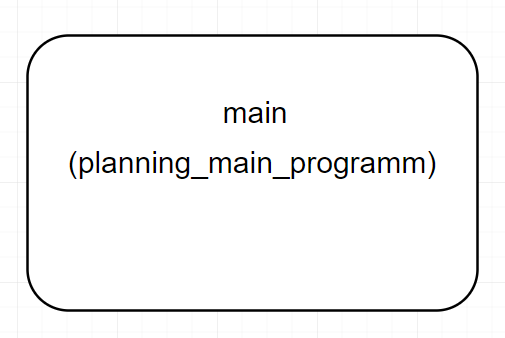
\includegraphics[width=0.4\textwidth]
        {img/diag_planning_main_programm.png}
        \caption{} Architektur der Quellcode-Datei main.lisp}
\end{figure}



\subsection{Beschreibung des Teilsystems}
\subsubsection{\"Ubersicht}
\chapterauthor{Kevin Störmer}
Die Quellcode-Datei 'main' im Paket 'planning\_main\_programm' soll ausschliesslich auf höchster Ebene den internen Ablauf des PR2 modellieren. 

Alle dafür notwendigen Logiken, die auf Basis externer Daten entschieden werden, wurden dabei basierend auf der Quelle der Daten in andere Quellcode-Dateien ausgelagert. Dabei wurde z.b der Vergleich zweier Punkte aus Vision in die Quellcode-Datei 'vision-communicate' (Paket: planning\_vision) ausgelagert. \\


Git-tag: Milestone 2:

\url{https://github.com/menanuni/planning_suturo_1718/releases/tag/0.2} \\

Git-tag Milestone 2 Branch TestObjectsPositioning aufgrund von merge Konflikten:

\url{https://github.com/menanuni/planning_suturo_1718/releases/tag/0.19}\\

\subsubsection{main ()}
\chapterauthor{Vanessa Hassouna}
\begin{verbatim}
main()
Die Main startet eine 'ros-node' mit dem Namen planning\_main.
Diese Node läuft solange,bis die komplette Main einmalig durchlaufen wurde. 
@return: T oder Nil 
\end{verbatim}



\subsection{Programmablauf}
\chapterauthor{Vanessa Hassouna}


\begin{figure}[!htb]
        \center{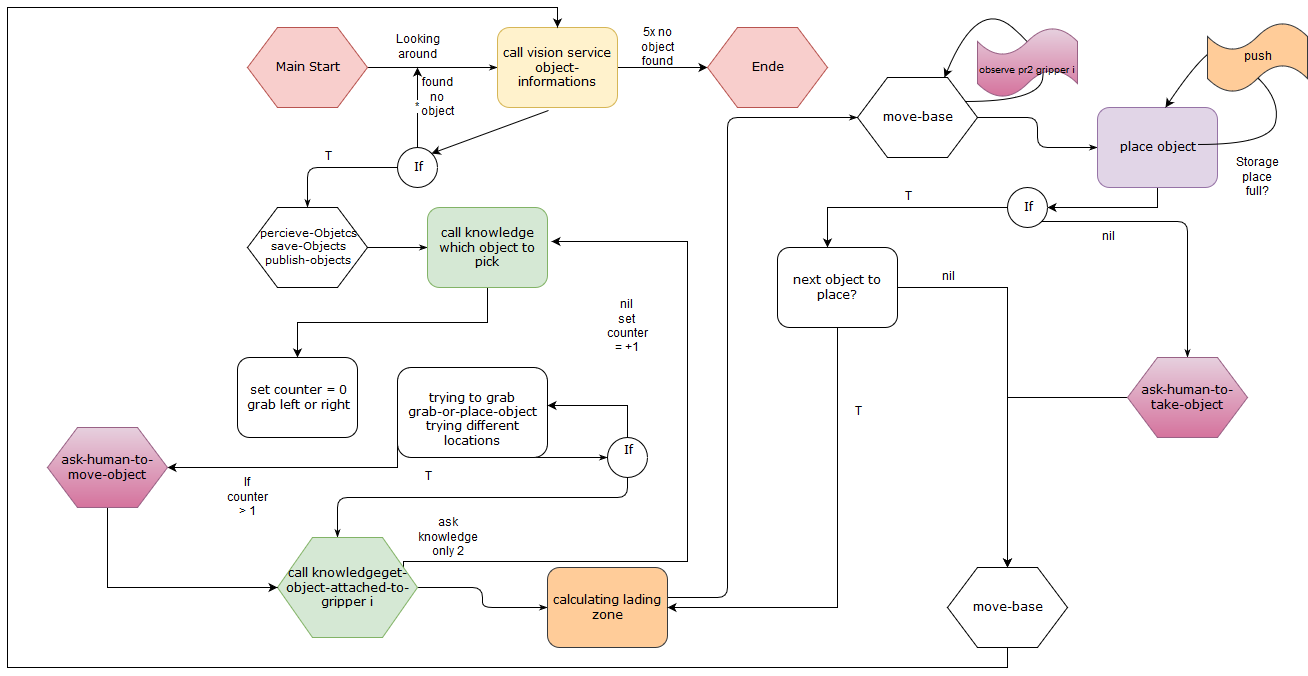
\includegraphics[width=1.0\textwidth]
        {img/vanessa_main.png}
        \caption{} Main-Diagramm von Vanessa.lisp}
\end{figure}





%müsste eigendlich wieder ausgelagert werden, kann von mir aus aber auch drin bleiben 
\subsubsection{find-Object(x z)}
\chapterauthor{Kevin Störmer}
\begin{verbatim}
find-Object()
Beschreibung: Sucht anhand variabler x und z-Achse sowie fest eingestellter
y-Koordinaten nach sichtbaren Objekten. Sollte ein Objekt gefunden werden,
oder die maximale Anzahl an Suchläufen überschritten werden,
terminiert die Funktion. Die Funktion beginnt immer beim zuletzt gesehenen Punkt.
@param: x-axis z-axis
@return: T wenn Objekt gefunden, nil falls nichts zu finden
\end{verbatim}




\newpage
\section{Die Quellcode-Datei: vision\_communicate.lisp (planning\_vision)}

\subsection{Architekturbild}

\chapterauthor{Vanessa Hassouna}



\begin{figure}[!htb]
        \center{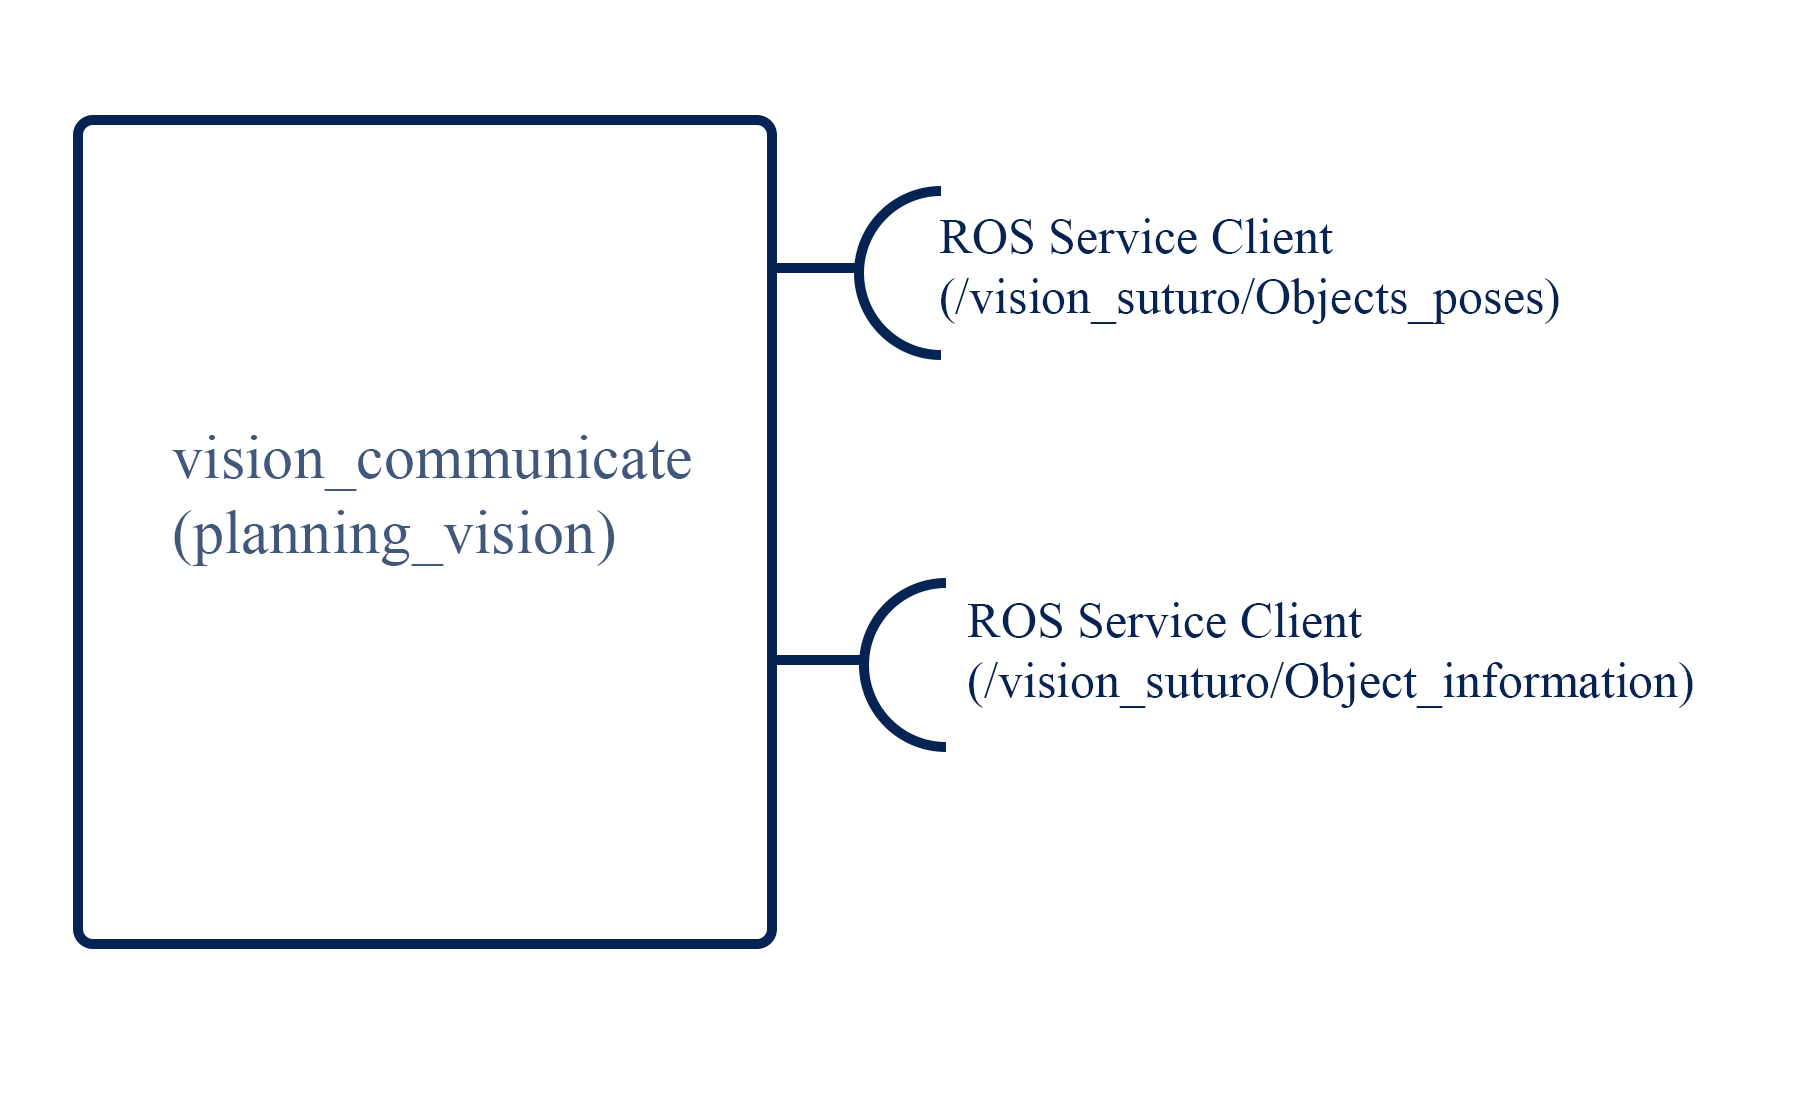
\includegraphics[width=0.6\textwidth]
        {img/vision.png}
        \caption{} Architektur der Quellcode-Datei vision\_communicate.lisp}
\end{figure}




\subsection{API}
\chapterauthor{Vanessa Hassouna}
\subsubsection{Serviceclients}
1. '/vision\_suturo/Object\_information' \\
Nimmt Objekt über Kinect wahr und gibt eine 'msg' zurück mit Informationen.\\ \\
2. '/vision\_suturo/objects\_pose' \\
Gibt zu einem Objekt (übergeben als Nummer) und einem Label (übergeben als String) die Pose mit Rotation zurück.

\subsection{Beschreibung des Teilsystems}




\subsubsection{call-Vision-Object-Clouds ()}
\chapterauthor{Vanessa Hassouna}
\begin{verbatim}
call-Vision-Object-Clouds ()

Beschreibung: Der Service von Vision "/vision\_suturo/objects\_information"
wird aufgerufen.

@return: Successfull oder Aborted
\end{verbatim}

%ausgelagert in planning_old
\subsubsection{check-Points-Is-Equal (msg-one msg-two delta))}
\chapterauthor{Kevin Störmer}
\begin{verbatim}
check-Points-Is-Equal (msg-one msg-two delta)

Beschreibung: Vergleicht 2 object_detection-srv:object in
ihren x, y, z Koordinaten anhand eines übergebenen Deltas.
Überschreitet die Differenz der beiden Messages das Delta
wird nil zurückgegeben.

@param: object_detection-srv:object msg-one 
object_detection-srv:object msg-two int delta
@return: T or nil
\end{verbatim}

\section{Die Quellcode-Datei: knowledge-communicate.lisp\\
planning\_knowledge)}

\subsection{Architekturbild}
\chapterauthor{Vanessa Hassouna}

\begin{figure}[!htb]
        \center{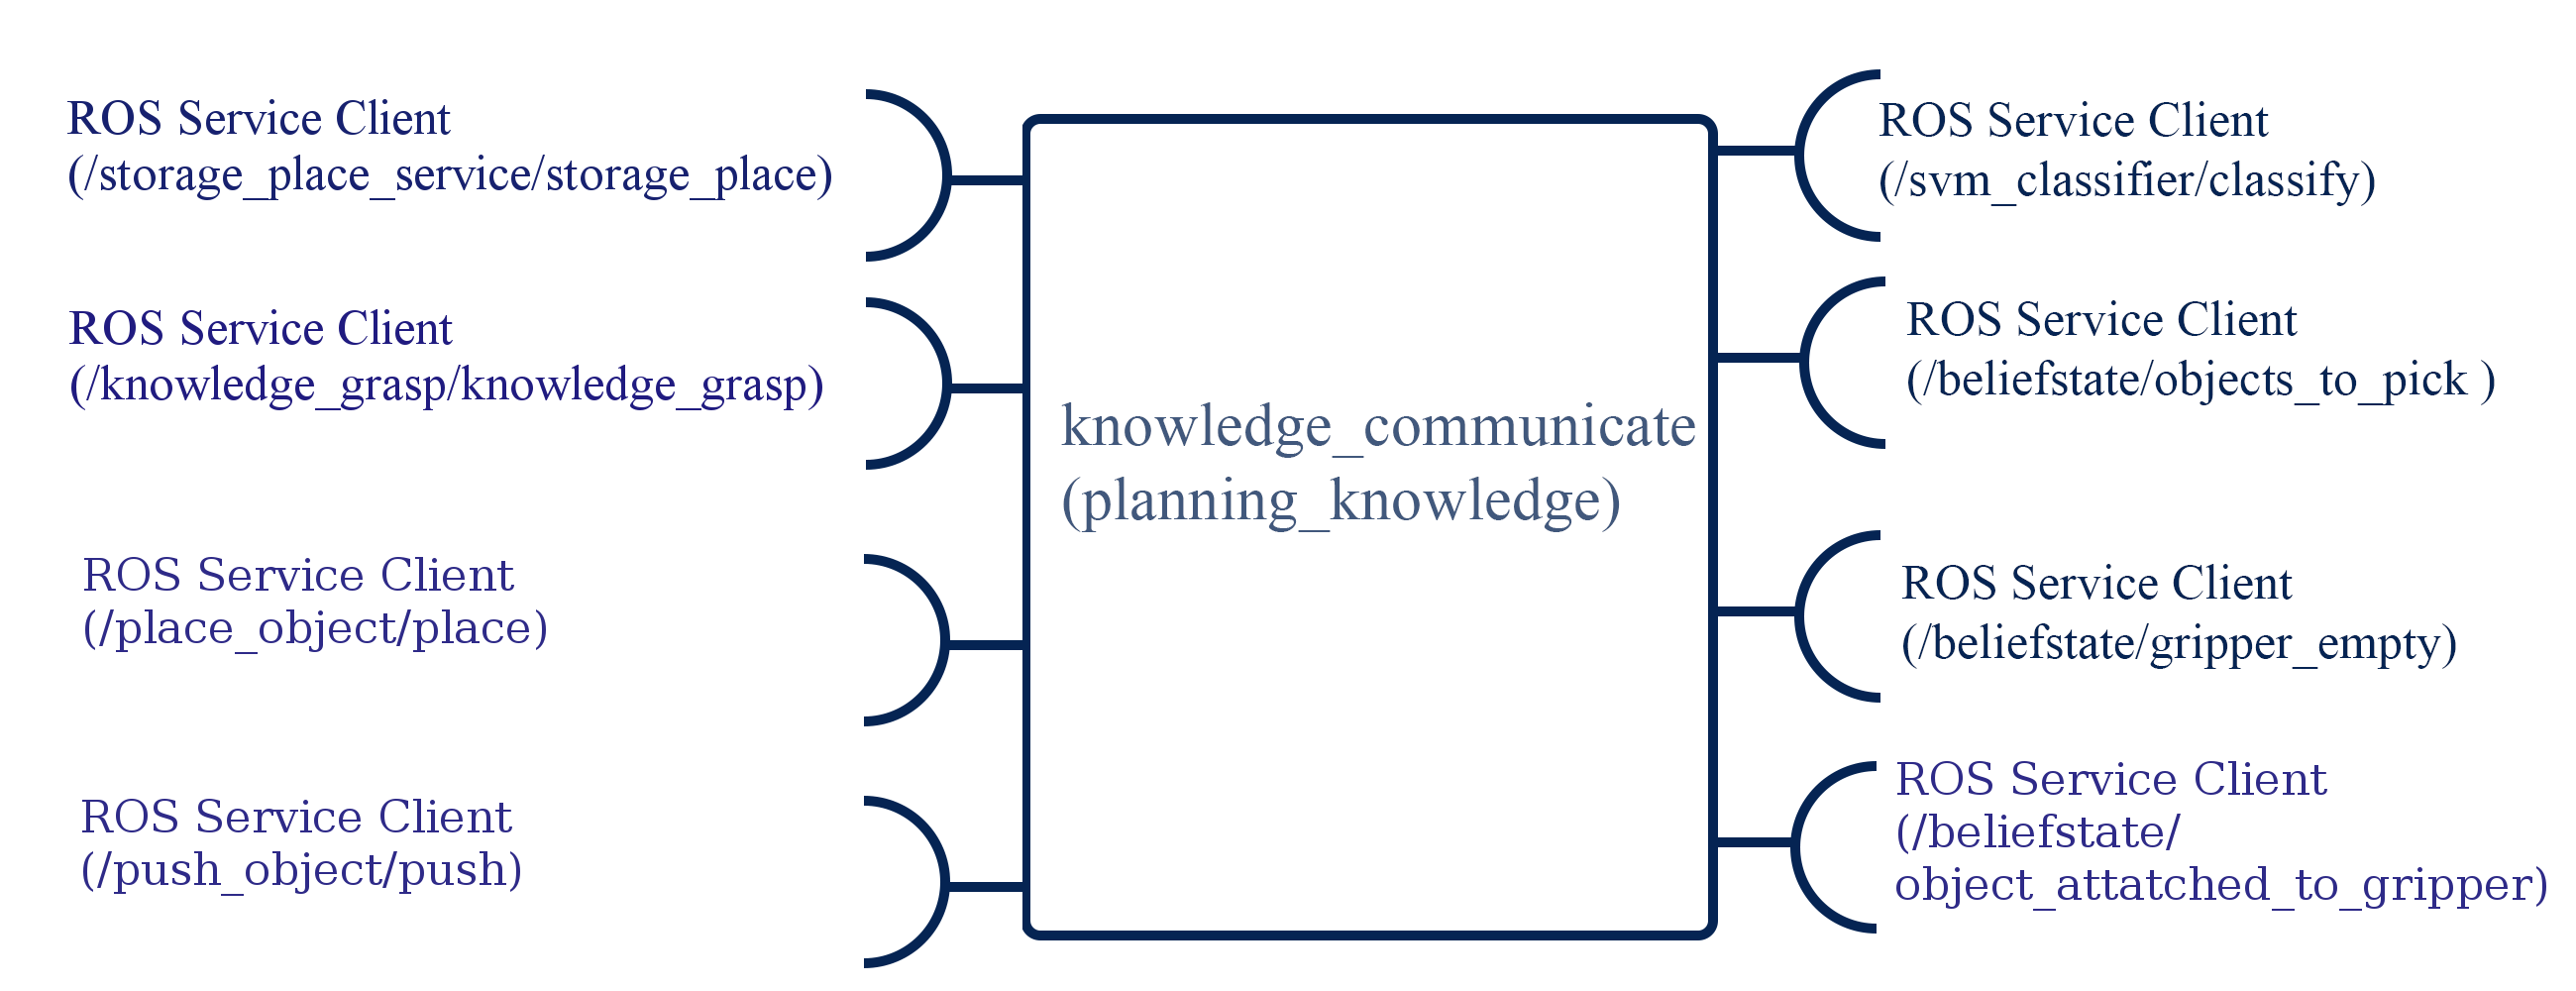
\includegraphics[width=1.0\textwidth]
        {img/knowledge.png}
        \caption{} Architektur der Quellcode-Datei knowledge-communicate.lisp}
\end{figure}

\subsection{API}
\chapterauthor{Vanessa Hassouna}
\subsubsection{Serviceclients}

1. 'beliefstate/objects\_to\_pick'\\
Gibt uns zwei Strings zurück. Diese sind leer, wenn kein Objekt mehr gegriffen werden soll oder es kein Objekt mehr zum Greifen gibt.

2. 'beliefstate/gripper\_empty'\\
Wir können erfragen, welcher Gripper frei ist.\\

3. 'kitchen\_mode\_service/get\_fixed\_kitchen\_objects'\\

4. 'storage\_place\_service/storage\_place'\\

5. 'knowledge\_grasp/knowledge\_grasp'\\

6. 'beliefstate/objects\_attached\_to\_gripper\\

\subsubsection{Topics}
1. 'beliefstate/perceive\_action'\\
Wenn ein Objekt wahrgenommen wurde, publishen wir diese Information.


\subsection{Beschreibung des Teilsystems}
\subsubsection{\"Ubersicht}
\chapterauthor{Kevin Störmer}
Die Quellcode-Datei 'knowledge-communicate' im Paket 'planning\_knowledge' ist ausschliesslich für die Kommunikation mit Modulen der Gruppe Knowledge zust\"andig.

\subsubsection{what-object(features)}
\chapterauthor{Kevin Störmer}
\begin{verbatim}
what-object(features)
Beschreibung: Ruft "/svm_classifier/classify_service" Service auf
@param: features
@return: identifikation
\end{verbatim}

\subsubsection{ask-knowledge-where-belongs-object()}
\chapterauthor{Hauke Tietjen}
\begin{verbatim}
ask-knowledge-where-belongs-object()

Beschreibung: Fragt den "storage_place" Service von Knowledge zu welchem
Abstellplatz das gegebene Objekt gehört.

@param object
@return: Abstellplatz als X- und Y-Koordinate in der Mitte, sowie
Breite und Höhe
\end{verbatim}


\subsubsection{how-To-Pick-Objects()}
\chapterauthor{Hauke Tietjen}
\begin{verbatim}
how-To-Pick-Objects()

Beschreibung: Fragt den "knowledge_grasp" Service wie das gegebene Objekt 
gegriffen werden soll. Der Service wird ausnahmsweise auch zum Abstellen 
des Objekts verwendet, weil aufgrund technischer Probleme noch kein
Service zum Abstellen bereitgestellt werden konnte.

@param object
@return: grasp pose
\end{verbatim}

%%%%%%%%%%%%%%%%%%%%%%%%%%%%%%%%%%%%%%%%%%%%%%%%%%%%%%%%%%%%%%%%%%%%%%%%%%%%%%

\section{Die Quellcode-Datei: motion-actions.lisp (planning\_motion)}
\subsection{Architekturbild}
\chapterauthor{Vanessa Hassouna}


\begin{figure}[!htb]
        \center{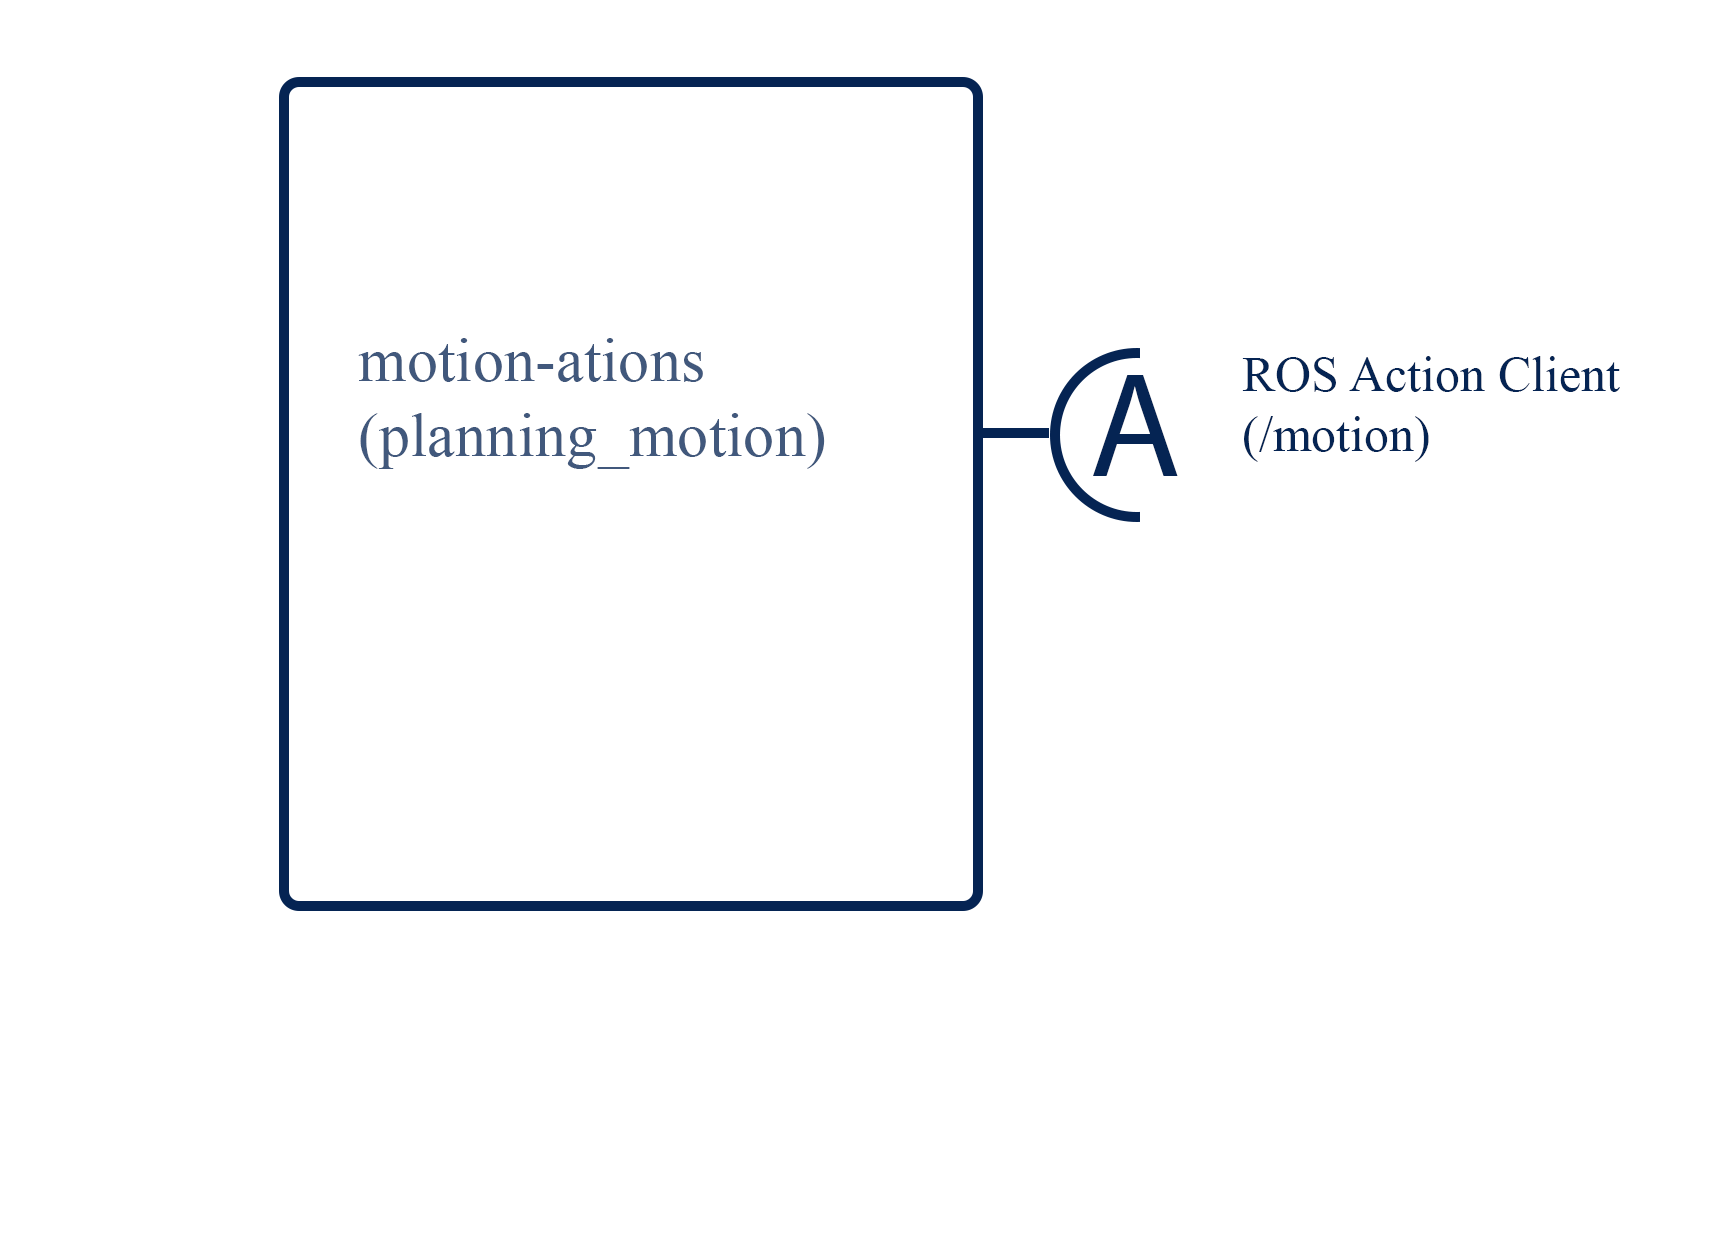
\includegraphics[width=0.6\textwidth]
        {img/motion.png}
        \caption{} Architektur der Quellcode-Datei motion-actions.lisp}
\end{figure}




\subsection{API}
\chapterauthor{Kevin Störmer}
\subsubsection{Actionclients}
1. '/motion' \\
Bewegt die Arme des Pr2 entweder in die Home-Position oder zu einem bestimmten Punkt.
\subsection{Beschreibung des Teilsystems}
\subsubsection{\"Ubersicht}
\chapterauthor{Kevin Störmer}
Die Quellcode-Datei 'motion-actions' im Paket 'planning\_motion'  ist ausschliesslich für die Kommunikation mit Modulen der Gruppe Motion zuständig. Dabei wird die Action '/motion' einmal für die Home-Position des Pr2, zum Bewegen des Armes zu einem bestimmten Punkt und zum Greifen genutzt.


\subsubsection{call-Motion-Move-Arm-Homeposition()}
\chapterauthor{Vanessa Hassouna und Hauke Tietjen}
\begin{verbatim}
call-Motion-Move-Arm-Homeposition()

Beschreibung: Ruft den Actionserver von Motion auf und
sendet das 'Command 2'.Dieses Command lässt die Arme des Pr2 
in die Homeposition fahren.

@return: Successfull oder Aborted
\end{verbatim}



\subsubsection{call-Motion-Move-Arm-To-Point \\
(point-center-of-object \&optional (x 3))
}
\chapterauthor{Vanessa Hassouna und Hauke Tietjen}
\begin{verbatim}
call-Motion-Move-Arm-To-Point (point-center-of-object \&optional (x 3))

Beschreibung: Ruft den Actionserver von Motion auf und 
sendet den Befehl einen Arm zu dem point-center-of-object zu fahren.

@param point-center-of-object &optional (x 3)
@return: Successfull oder Aborted
\end{verbatim}

\newpage
\section{Die Quellcode-Datei: movement.lisp (planning\_move)}
\subsection{Architekturbild}
\chapterauthor{Kevin Störmer}


\begin{figure}[!htb]
        \center{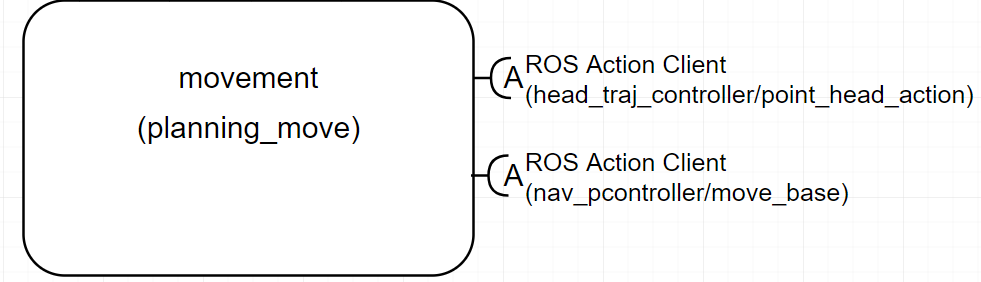
\includegraphics[width=0.8\textwidth]
        {img/diag_planning_move.png}
        \caption{} Architektur der Quellcode-Datei movement.lisp}
\end{figure}


\subsection{API}
\chapterauthor{Kevin Störmer}
\subsubsection{Actionclients}
1. 'head\_traj\_controller/point\_head\_action' \\
Bewegt den Kopf des Pr2 in Richtung eines Punktes.\\ \\
2. 'nav\_pcontroller/move\_base' \\
Bewegt die Basis des Pr2 in Richtung eines Punktes.
\subsection{Beschreibung des Teilsystems}

\subsubsection{\"Ubersicht}
\chapterauthor{Kevin Störmer}
Die Quellcode-Datei actions.lisp im Paket 'planning\_motion'  ist ausschliesslich für die Kommunikation mit Gruppe Motion zuständig. Dabei wird die Action '/motion' einmal für die Home-Position des Pr2 und zum Bewegen des Armes zu einem bestimmten Punkt genutzt.



\subsubsection{move-head (x y z)}
\chapterauthor{Kevin Störmer}

\begin{verbatim}
move-Head (x y z)
Beschreibung: Lässt den Rr2-Kopf bewegen, dabei wird der Service 
"head_traj_controller/point_head_action" angesprochen.
x,y, und z werden als Koordinaten ausgehend von base_link behandelt.
@param: x y z
@return: Succesfull oder Aborted
\end{verbatim}



\subsubsection{move-Base-To-\\
Point (x y z angle)}
\chapterauthor{Vanessa Hassouna}
\begin{verbatim}
move-Base-To-Point (x y z angle)

Beschreibung: Anhand des Actionservice "nav\_pcontroller/move\_base" 
wird die Basis bewegt. Der Punkt und die Rotation sind in Frame "map" anzugeben.

@param: x y z angle
@return: Successfull oder Aborted
\end{verbatim}


\subsubsection{move-Robo-Into-Homeposition ()}
\chapterauthor{Vanessa Hassouna}
\begin{verbatim}
move-Robo-Into-Homeposition ()

Beschreibung: move-Base-To-Point wird aufgerufen mit 
von uns vordefinierten Punkten, die als Homeposition dienen.

@return: Succesfull oder Aborted
\end{verbatim}



\subsubsection{init-Action-Client-Base ()}
\chapterauthor{Vanessa Hassouna}
\begin{verbatim}
init-Action-Client-Base ()

Beschreibung: Diese Hilfsfunktion dient dazu, 
den Action-Client zu initialisieren.

@return: Successfull oder Aborted
\end{verbatim}

\subsubsection{get-Action-Client-Base ()}
\chapterauthor{Vanessa Hassouna}
\begin{verbatim}
get-Action-Client-Base ()

Beschreibung: Diese Hilfsfunktion dient dazu, den Action-Client zu erhalten.

@return: Successfull oder Aborted
\end{verbatim}





\section{Die Quellcode-Datei: external-logic.lisp (planning\_logic)}
\subsection{Architekturbild}
\chapterauthor{Vanessa Hassouna}


\begin{figure}[!htb]
        \center{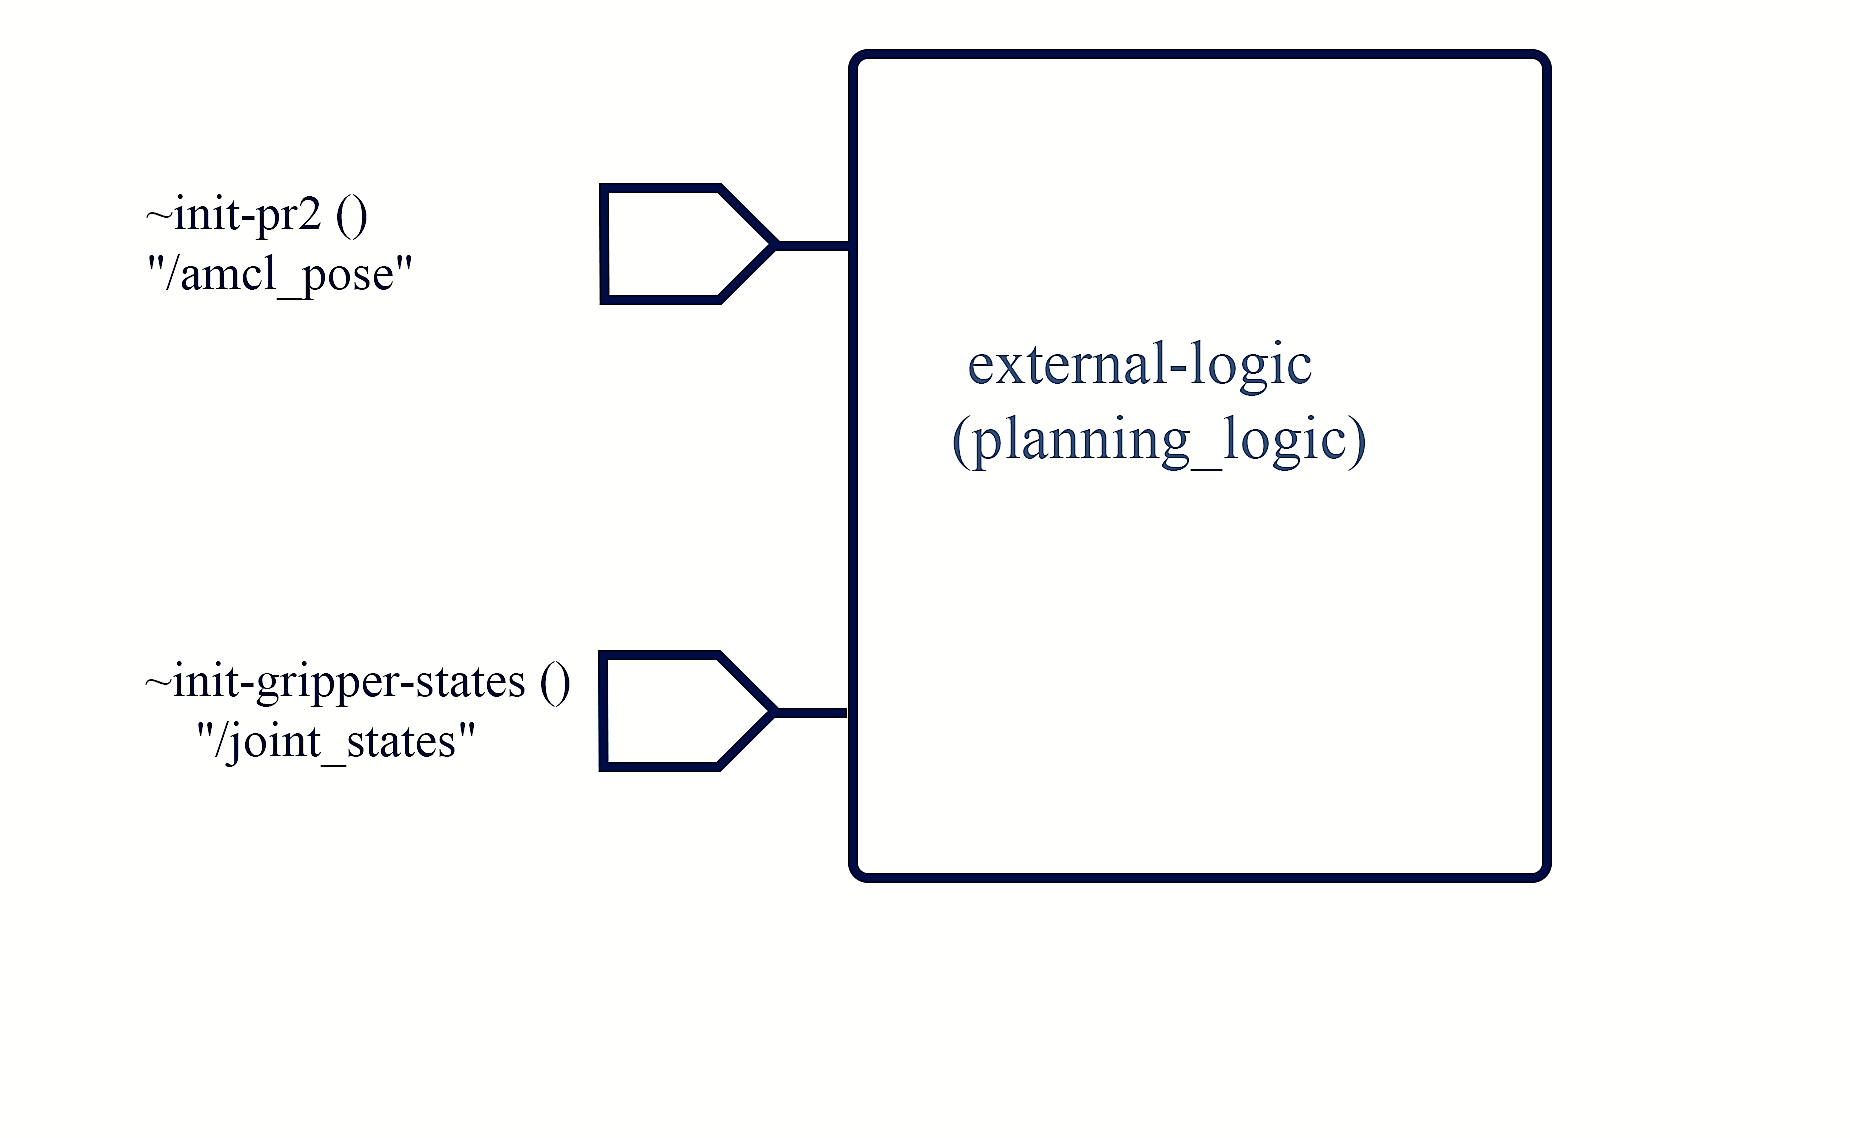
\includegraphics[width=0.8\textwidth]
        {img/externallogic.png}
        \caption{} Architektur der Quellcode-Datei movement.lisp}
\end{figure}


\subsection{API}
\chapterauthor{Vanessa Hassouna}
\subsubsection{Topics}
1. 'joint\_states' \\
Subscribed das Topic und speichert die Werte des Grippers.\\
 
2. 'robot\_pose' \\
Subscribed das Topic und gibt uns die Position des Roboters zurück.
\subsection{Beschreibung des Teilsystems}

\subsubsection{\"Ubersicht}
\chapterauthor{Vanessa Hassouna}
Die Quellcode-Datei 'external-logic.lisp' im Paket 'planning\_logic' ist für reine logische Funktionen vorgesehen.



\subsubsection{transformation-Vision-Point (pose amount\\
\&optional (endFrame '/base\_footprint')}
\chapterauthor{Vanessa Hassouna}
\begin{verbatim}
transformation-Vision-Point (pose amount &optional (endFrame "/base\_footprint")

Beschreibung: Das gegebene Objekt wird von dem ausgehenden Frame
in ein optionales Frame umgewandelt.

@param: pose, amount und optional endFrame
@return: Liefert eine transformierte tf-point-stamped
\end{verbatim}


\subsubsection{publish-pose (label object\_pose)}
\chapterauthor{Kevin Störmer}
\begin{verbatim}
publish-pose (label object_pose)

Beschreibung: Published eine knowledge_msgs/PerceivedObject-msg

@param: string label, PoseStamped object_pose
@return: int amountOfListeners
\end{verbatim}


\subsubsection{ publish-Text (string)}
\chapterauthor{Vanessa Hassouna}
\begin{verbatim}
publish-Text (string)

Beschreibung: Publisht einen Text in RVIZ mit einem übergebenen String.

@param:string
\end{verbatim}


\subsubsection{publish-Pose-JaMilch ()}
\chapterauthor{Vanessa Hassouna}
\begin{verbatim}
publish-Pose-JaMilch ()

Beschreibung: Die Funktion ist nur für das Demoszenario 
erstellt. Eine "JaMilch" wir "gesehen" und gepublisht
an das Team Knowledge. Es wird auche in neuer Parameter
auf dem Paramserver erstellt der den Namen des Strings
bekommt.

@param:string
\end{verbatim}



\subsubsection{catch-Transformation \\
(transform-listener tf-point-stamped endFrame)}
\chapterauthor{Vanessa Hassouna}
\begin{verbatim}
catch-Transformation (transform-listener tf-point-stamped endFrame)

Beschreibung: Hier findet die eigentliche Transformation, von der
Funktion transformation-Vision-Point 
pose amount &optional (endFrame "/base_footprint"), statt.

@param: transform-listener tf-point-stamped endFrame
@return: Liefert eine transformierte tf-point-stamped
\end{verbatim}

\subsubsection{disassemble-graspindividual-response (msg)}
\chapterauthor{Kevin Störmer}
\begin{verbatim}
disassemble-graspindividual-response (msg)

Beschreibung: Löst die Y-Koordinate einer GraspPose heraus.

@param: GraspPoseMessage msg
@return: float y
\end{verbatim}


\subsubsection{transformation-XYZ (x y z startFrame\\
\&optional (endFrame '/base\_footprint'))}
\chapterauthor{Vanessa Hassouna}
\begin{verbatim}
transformation-XYZ (x y z startFrame &optional (endFrame "/base_footprint"))

Beschreibung: Transformiert einen Punkt mit dem standart
Quaternion  0 0 0 1.

@param: x y z startFrame &optional (endFrame "/base_footprint")
@return: Liefert eine transformierte tf-pose-stamped
\end{verbatim}


\subsubsection{ transformation-Pose-Stamped \\
(pose \&optional (endFrame '/base\_footprint')) }
\chapterauthor{Vanessa Hassouna}
\begin{verbatim}
 transformation-Pose-Stamped (pose &optional (endFrame "/base_footprint")) 

Beschreibung: Transformiert eine Pose-Stamped-msgs mit einem optional Frame,\\
 default ist base_footprint.

@param: x y z startFrame &optional (endFrame '/base_footprint')
@return: Liefert eine transformierte tf-pose-stamped
\end{verbatim}




\subsubsection{make-Object-Pose-For-Handshake (label)}
\chapterauthor{Vanessa Hassouna}
\begin{verbatim}
make-Object-Pose-For-Handshake (label)

Beschreibung: Erstellt eine msg von dem Punkt eines Objektes\\ 
für die Handshake Methode.

@param: label
@return: T oder Nil
\end{verbatim}

\subsubsection{ percieve-Objetcs ()}
\chapterauthor{Vanessa Hassouna}
\begin{verbatim}
percieve-Objetcs ()

Beschreibung: Ruf vision_suturo Service um Objekte wahrzunehmen auf\\
wärend dessen wir durch die größe des übergebenen Arrays \\
durchgelaufen und jedes gesehene Objekt gepublisht, sowie\\
auf dem Paramserver gespeichert. Auch ein Counter wird gesetzt\\
der mitzählt wieviele Objekte gesehen wurden.

@return: T oder Nil
\end{verbatim}

\subsubsection{ percieve-Objects-And-Search (label)}
\chapterauthor{Vanessa Hassouna}
\begin{verbatim}
 percieve-Objects-And-Search (label)

Beschreibung: Sucht nach einem Objekt ob es noch gesehen wird.
@param: label
@return: T oder Nil
\end{verbatim}


\subsubsection{get-Information-About-Object (label)}
\chapterauthor{Vanessa Hassouna}
\begin{verbatim}
get-Information-About-Object (label)

Beschreibung: Transformiert einen Punkt von dem gegeben Objekt\\
in den Frame "Map".

@param: label
@return: Transformed y
\end{verbatim}

\subsubsection{save-Object (label object\_pose)}
\chapterauthor{Vanessa Hassouna}
\begin{verbatim}
save-Object (label object_pose)

Beschreibung: Das gegeben Objekt wird auf dem \\
Paramserver gespeichert. Hier wird jedoch nur der Punkt\\
des Objektes berücksichtigt und der Name des Parameters \\
ist der Name des Objektes.

@param: label object_pose
@return: T oder Nil
\end{verbatim}


\subsubsection{init-Marker ()}
\chapterauthor{Vanessa Hassouna}
\begin{verbatim}
init-Marker ()

Beschreibung: Subscribed das Topic '/visualization_markers'.

@return: geometry_msgs/Pose
\end{verbatim}

\subsubsection{init-pr2()}
\chapterauthor{Vanessa Hassouna}
\begin{verbatim}
init-pr2 ()

Beschreibung: Subscribed das Topic '/amcl_status'.

@return: geometry_msgs/Pose
\end{verbatim}

\subsubsection{pose-cb (msg)}
\chapterauthor{Vanessa Hassouna}
\begin{verbatim}
pose-cb (msg)

Beschreibung: Callback-Funktion für die Funktion init-pr2().

@param: msg
@return: geometry_msgs/Pose
\end{verbatim}

\subsubsection{move-pr2 (x y z)}
\chapterauthor{Vanessa Hassouna}
\begin{verbatim}
move-pr2 (x y z)

Beschreibung: Bewegt den Roboter zu einem Punkt, wenn dieser hinter\\
dem Roboter liegt begiebt dieser sich erst in eine Safeposition.
@param: x y z 
@return: Successfull oder Aborted
\end{verbatim}

\subsubsection{angle-From-Pr2-Pose-To-Point (x-goal y-goal z-goal)}
\chapterauthor{Vanessa Hassouna}
\begin{verbatim}
angle-From-Pr2-Pose-To-Point (x-goal y-goal z-goal)

Beschreibung: Die Funktion arbeitet mit Hilfe des Packets Cram-Language um 
einen Winkel zu berechnen, wie der Pr2 sich aus der aktuellen Position 
in der Welt drehen muss, damit er einen gegebenen Punkt erreichen kann.
Da der Roboter sich in dem Frame "map" bewegt, muss der Winkel noch mit der 
aktuellen Orientierung des Pr2 subtrahiert werden, so dass am Ende
ein Winkel resultiert der in dem Frame "map" funktioniert.

@param: x-goal y-goal z-goal 
@return: angle 
\end{verbatim}


\subsubsection{should-Robo-Use-Left-Or-Right-Arm(pose amount \\
\&optional (endFrame '/base\_footprint'))}
\chapterauthor{Vanessa Hassouna}
\begin{verbatim}
should-Robo-Use-Left-Or-Right-Arm (pose amount &optional
(endFrame "/base_footprint"))

Beschreibung: Anhand der Y-Achse entscheidet der Roboter
ob er den linken oder rechten Arm bewegen soll.

@param: pose object-number &optional endFrame
@return: 3 oder 2 (3 = links 2 = Rechts)
\end{verbatim}

\subsubsection{ try-To-Grab-Or-Place-Different-Location\\
(x y z w label command)}
\chapterauthor{Vanessa Hassouna}
\begin{verbatim}
try-To-Poke-Different-Location\\
(point-for-motion number-for-arm)

Beschreibung: Die Funktion lässt den Roboter 
anhand vorgegebener Positionen seine Drehung sowie seine
Position ändern, wenn er ein Objekt nicht erreichen kann.
Achtung die X-, Y-, Z- und W-Werte müssen in dem Frame "map" angegeben werden.
Der Roboter selber bewegt sich in dem Map base\_footprint.

@param: x, y, z, w, label, command
@return: T oder Nil


\end{verbatim}

\subsubsection{  grab-Or-Place-Object (label x y angle arm-first \\
arm-first-homeposi grab-string \&optional \\
arm-second arm-second-homeposi)}
\chapterauthor{Vanessa Hassouna}
\begin{verbatim} 
grab-Or-Place-Object (label x y angle arm-first 
arm-first-homeposi grab-string &optional arm-second arm-second-homeposi)

Beschreibung: Versucht zu Greifen oder Abzustellen. Wenn der \\
übergebene String äquivalent zu "grab" ist, wird der Roboter \\
auch mit dem zweiten Arm versuchen zu Greifen, wenn der erste\\
nicht Funktioniert hat.

@param: label x y angle arm-first arm-first-homeposi grab-string &optiona\\
arm-second arm-second-homeposi
@return: T oder Nil
\end{verbatim}



\subsubsection{ trying-To-Grab (label x y angle arm-first arm-first-homeposi \\
grab-string arm-second arm-second-homeposi)}
\chapterauthor{Vanessa Hassouna}
\begin{verbatim} 
 trying-To-Grab (label x y angle arm-first arm-first-homeposi
 grab-string arm-second arm-second-homeposi)

Beschreibung: Ruft grab-or-place-object auf, wenn der \\
Caounter größer ist als 0 verändert der Pr2 seine Position \\
und setzt den Counter auf 1, damit er in keinen Loop gerät.

@param: Label x y angle arm-first arm-first-homeposi \\
grab-string arm-second arm-second-homeposi
@return: T oder Nil
\end{verbatim}

\subsubsection{how-Many-Gripper ()}
\chapterauthor{Vanessa Hassouna}
\begin{verbatim} 
how-Many-Gripper ()

Beschreibung: Durchläuft den empty-gripper server\\
und setzt die Variablen für Linken- und Rechten-arm auf \\
T oder Nil.

@return: T oder Nil
\end{verbatim}


\subsubsection{calculate-Object-And-Pr2-Distance (label)}
\chapterauthor{Vanessa Hassouna}
\begin{verbatim} 
calculate-Object-And-Pr2-Distance (label)

Beschreibung: Berechnet die Distanz zwischen dem \\
Pr2 und dem Objekt.

@param: label
@return: T oder Nil
\end{verbatim}


\subsubsection{distance (xa ya xb yb)}
\chapterauthor{Vanessa Hassouna}
\begin{verbatim}
distance (xa ya xb yb)

 Beschreibung: Berechnet die Distanz\\
zwischen zwei Vektoren.

@param: xa ya xb yb (vektor1 vektor2)
@return: distance
\end{verbatim}


\subsubsection{set-First-Posi ()}
\chapterauthor{Vanessa Hassouna}
\begin{verbatim}
set-First-Posi ()

 Beschreibung: Setzt die Globalen Variablen *x* und *y*\\
auf die erste Position (Die Position ist fest in der \\
Küche gewählt).

@return: T oder Nil
\end{verbatim}


\subsubsection{set-Second-Posi ()}
\chapterauthor{Vanessa Hassouna}
\begin{verbatim}
set-Second-Posi ()

 Beschreibung: Setzt die Globalen Variablen *x* und *y*\\
auf die zweite Position (Die Position ist fest in der \\
Küche gewählt).

@return: T oder Nil
\end{verbatim}





\subsubsection{init-gripper-states ()}
\chapterauthor{Kevin Störmer}
\begin{verbatim}
init-gripper-states ()
Beschreibung: Subscribed das Topic '/joint_states' und gibt als Callback-Funktion
'is-gripper-filled (msg)' an.
\end{verbatim}

\subsubsection{is-gripper-filled (msg)}
\chapterauthor{Kevin Störmer}
\begin{verbatim}
is-gripper-filled (msg)
Beschreibung: Aktualisiert alle 0.01 Sekunden die Fluents *gripper-righ-state-fluent* 
und *gripper-left-state-fluent* um T oder nil. Dabei wird anhand der Joint-States der
Gripper-Joints 'r_gripper_joint' und 'l_gripper_joint' entschieden
ob jeder Gripper des Pr2 gefüllt ist, oder nicht. Diese werte werden
aus den Joint-States geparsed.
@param: sensor_msgs/JointState msg 
\end{verbatim}



\section{Die Quellcode-Datei: objects.lisp (planning\_objects)}
\subsection{Architekturbild}
\chapterauthor{Hauke Tietjen}



\begin{figure}[!htb]
	\center{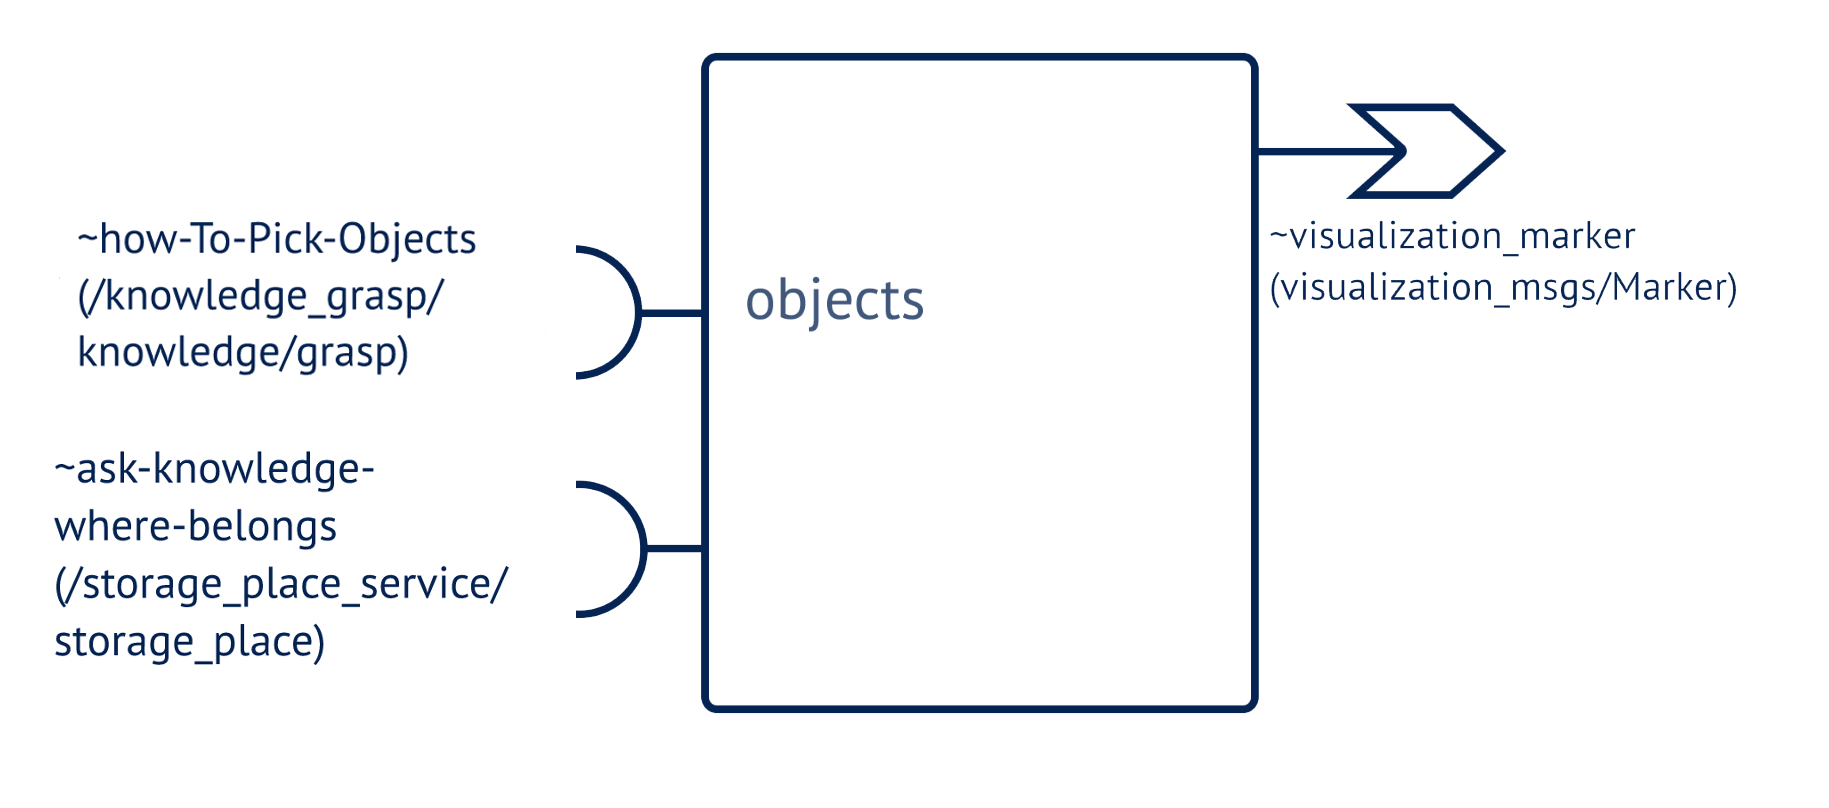
\includegraphics[width=1.1\textwidth]
		{img/diag_planning_objects.png}
		\caption{} Architektur der Quellcode-Datei planning-objects.lisp}
\end{figure}


\subsection{API}
\chapterauthor{Hauke Tietjen}
\subsubsection{Serviceclients}
1. '/storage\_place\_service/storage\_place' \\
Gibt den Ablageplatz des Objekts zur\"uck.\\ \\
2. '/place\_object/place' \\
Gibt die Pose zum abstellen eines Objektes zur\"uck\\ \\
3. '/beliefstate/gripper\_empty' \\
Gibt eine Message zurück die aussagt welcher Gripper leer ist\\ \\
4. '/push\_object/push' \\
Gibt eine Pose zum Verschieben des Objektes zur\"uck\\ \\
5. '/motion\_msgs/MovingCommandAction' \\
Bewegt den Gripper zur gegebenen Pose\\ \\
6. '/motion\_msgs/GripperAction' \\
Öffnet oder schließt die Hand auf das gegebene Maß\\ \\
7. 'visualization\_msgs/Marker' \\
Publiziert Marker zur Visualisierung von Landezonen.

\subsection{Beschreibung des Teilsystems}
\subsubsection{\"Ubersicht}
\chapterauthor{Hauke Tietjen}
Die Datei 'objects' aus dem Paket 'planning\_objects' dient dazu, aus den von Knowledge vorgegebenen Ablageorten für Objekte, Punkte zu bestimmen, die geeignet sind um Objekte auf ihnen abzustellen. Dabei werden Platzmangel und die Kollision von Objekten berücksichtigt. Zusätzlich lassen sich die finalen Positionen in Rviz visualisieren. Außerdem können Objekte nach hinten verschoben werden um Platz für Neue zu schaffen.

\subsubsection{calculate-landing-zone()}
\chapterauthor{Hauke Tietjen}
\begin{verbatim}
calculate-landing-zone()

Beschreibung: Zuerst wird überprüft ob der Parameter 'object' korrekt 
geschrieben wurde. Falls nicht wird ein Fehler ausgegeben. 
Die globale variable '*current-object-lable*' wird mit dem Parameter 
'object' befüllt. Die Funktion fragt Knowledge an welchen Ablageort 
das Objekt gehört und verkleinert ihn. Dadurch soll das Platzieren von 
Objekten auf Tischkanten und Wänden verhindert werden. Danach wird die 
Funktion fill-landing-zone-horizontally aufgerufen, die eine Pose 
zurück gibt. Die X- und Y-Koordinaten dieser Pose werden an Knowledge, 
mit einer weiteren Message welche die Grippernummer enthält,
weitergegeben. Knowledge gibt dann eine entsprechende Greifpose für 
das Objekt zurück. Die Pose wird mit dem String der die Kapazität 
des storage place beschreibt in eine Liste geschrieben und diese
zurückgegeben.

@param object
@return Gibt die Pose eines Grippers in /map zurück um ein Objekt abzustellen
\end{verbatim}

\begin{figure}[!htb]
	\center{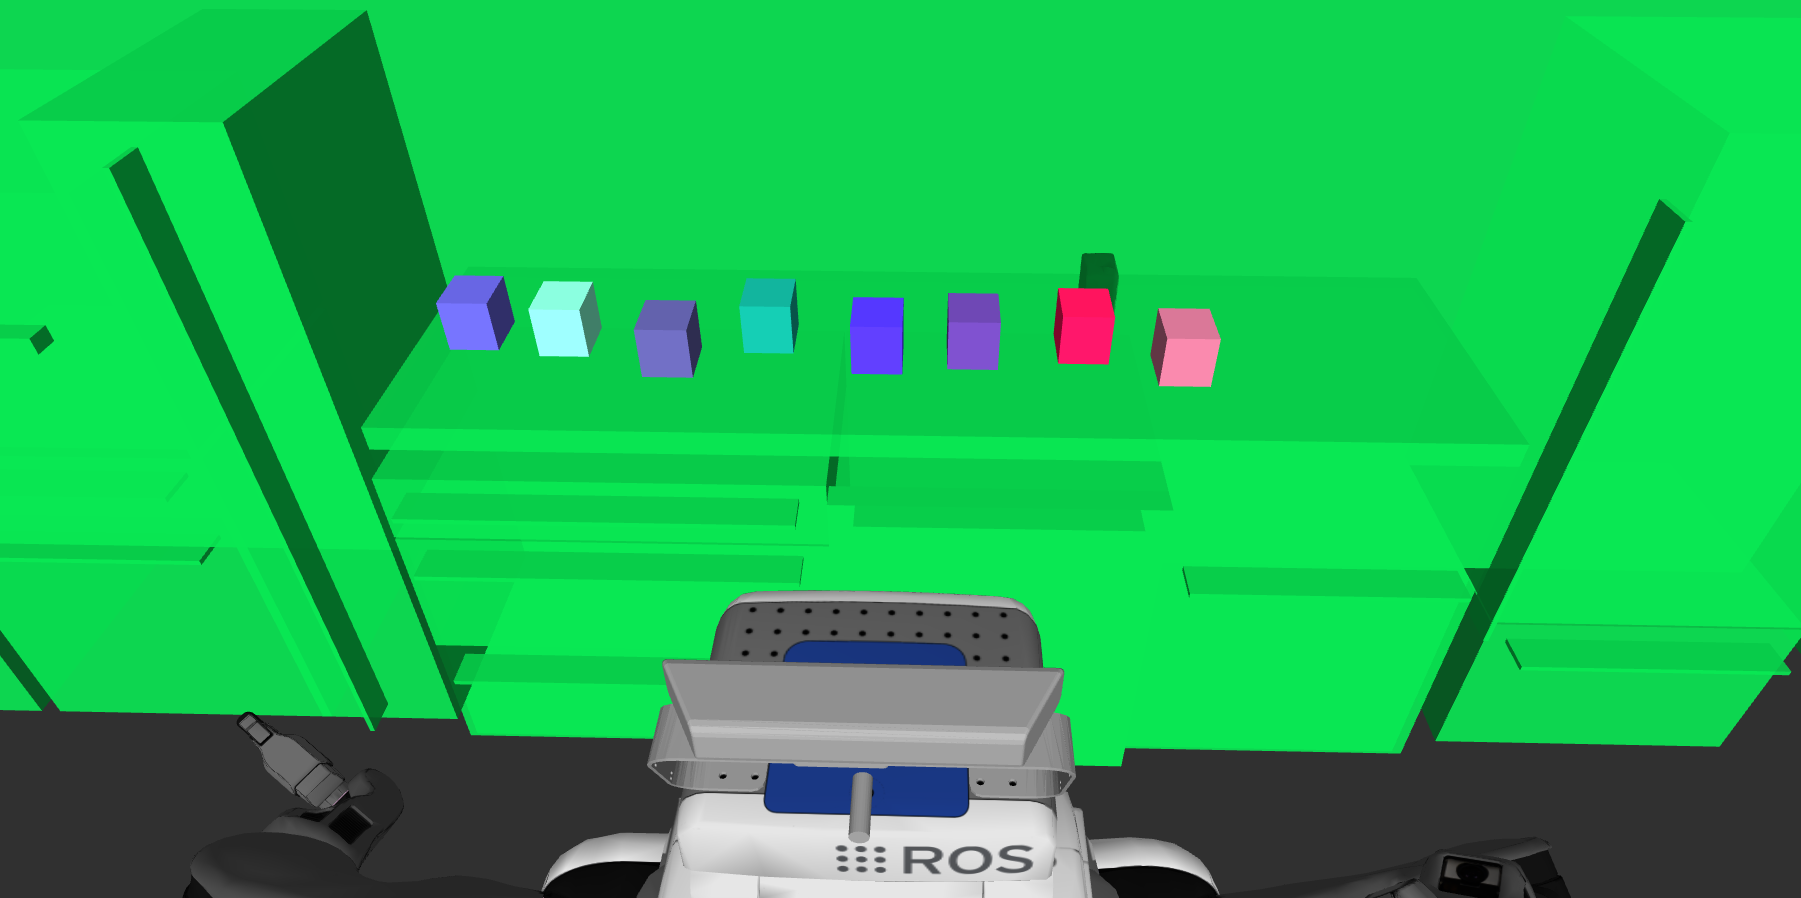
\includegraphics[width=1.0\textwidth]
		{img/objects_all_placed.png}
		\caption{} Alle Objekte in ihren Abstellzonen}
\end{figure}

\subsubsection{check-storage-place-spelling()}
\chapterauthor{Hauke Tietjen}
\begin{verbatim}
check-storage-place-spelling()

Beschreibung: Diese Funktion überprüft ob der Parameter 'object-label'
einem der Namen für Objekte entspricht. Der Name muss korrekt geschrieben
werden, weil sonst Knowledge den Namen nicht kennt und abstürzt. 
Die Namen sind: "HelaCurryKetchup", "TomatoSauceOroDiParma", 
"PringlesPaprika", "PringlesSalt", "JaMilch", 
"KoellnMuesliKnusperHonigNuss", "KellogsToppasMini", "CupEcoOrange", 
"EdekaRedBowl" und "SiggBottle".

@param object-label
@return true wenn es den Namen gibt, false falls nicht
\end{verbatim}

\subsubsection{fill-landing-zone-horizontally()}
\chapterauthor{Hauke Tietjen}
\begin{verbatim}
fill-landing-zone-horizontally()

Beschreibung: Es wird festgestellt in welchen Abstellbereich das Objekt gehört.
Dann wird überprüft ob noch genug Platz für das derzeitige Objekt und das 
Nächste ist. Dann wird der Bereich mit dem gegebenen Objekt befüllt.
Dies geschieht von positiv nach negativ auf der Y-Achse, im Frame '/map'.
Danach wird die erstellte Pose zurückgegeben.

@param position width height, der Landezone
@return Gibt eine Pose in /map zurück um ein Objekt abzustellen
\end{verbatim}

\begin{figure}[!htb]
	\center{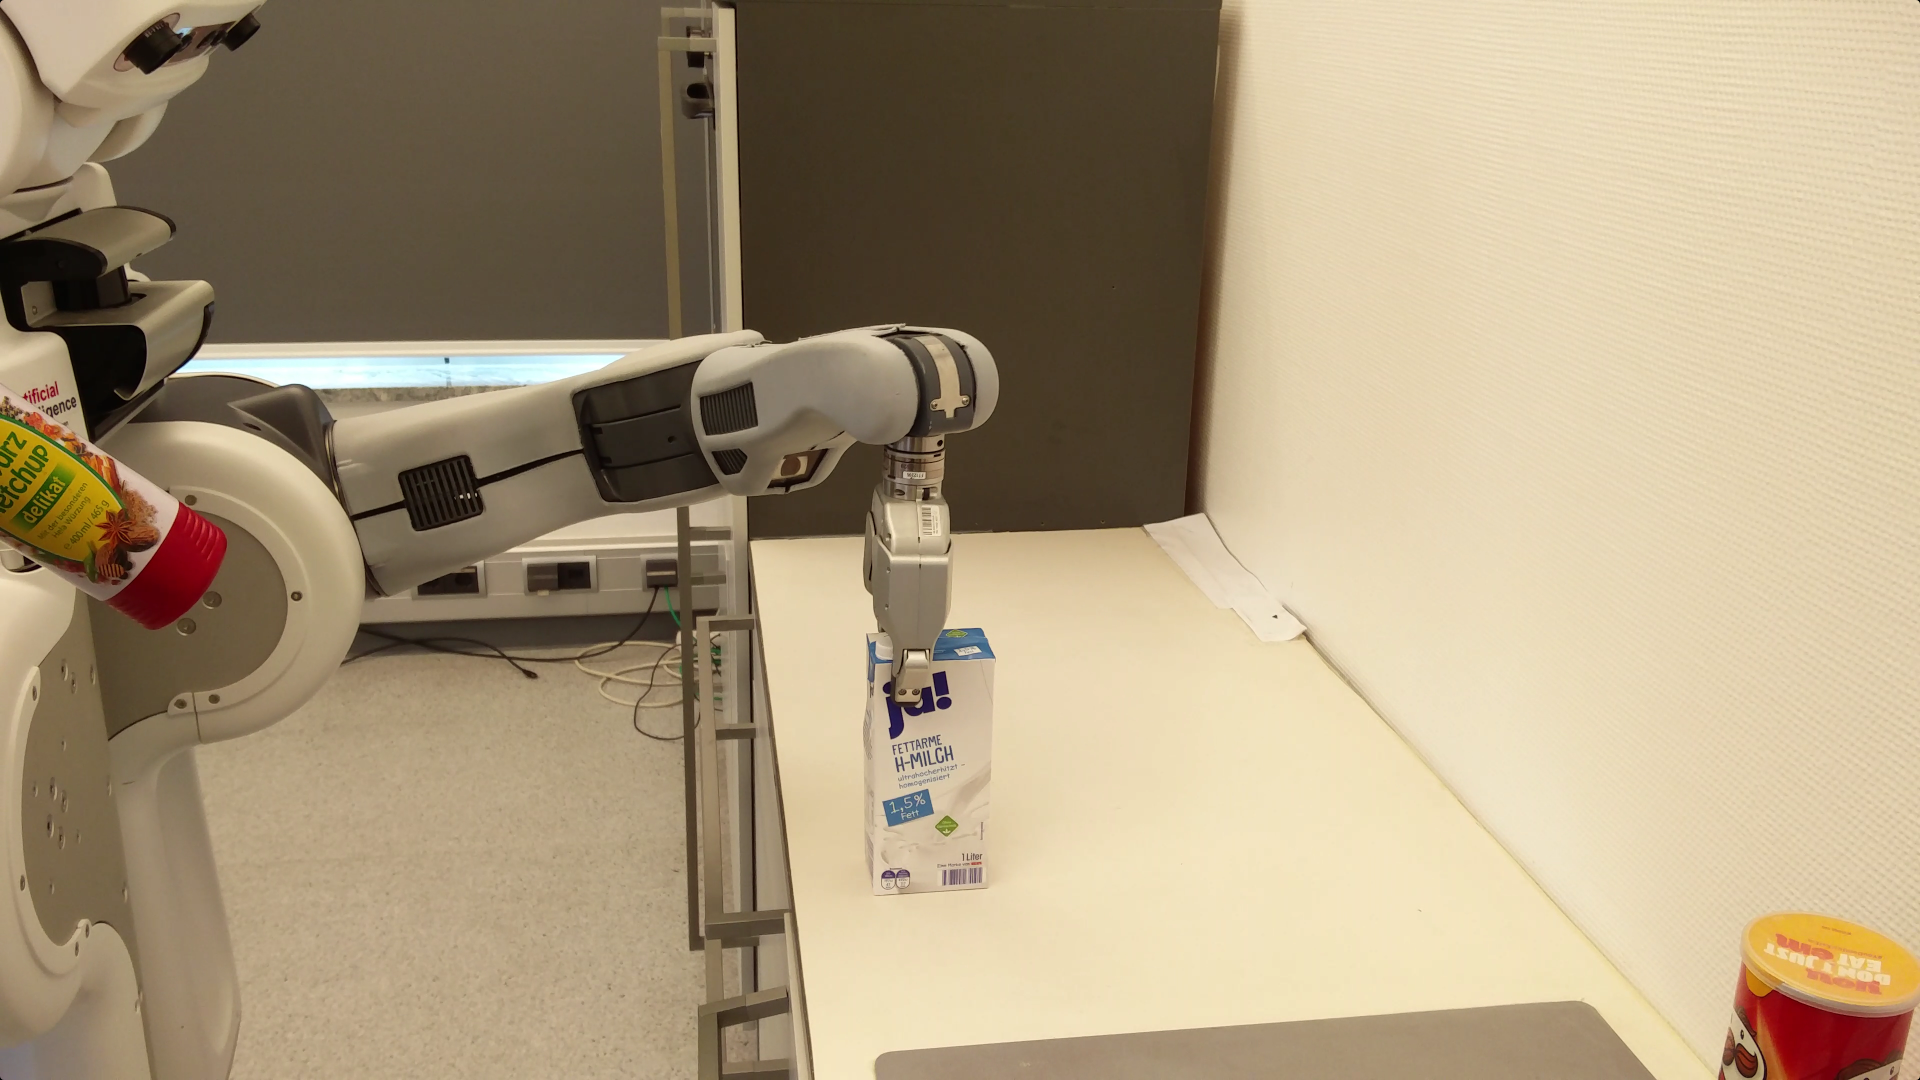
\includegraphics[width=1.0\textwidth]
		{img/objects_abstellen.png}
		\caption{} Das Abstellen eines Objekts}
\end{figure}

\subsubsection{push-object()}
\chapterauthor{Hauke Tietjen}
\begin{verbatim}
push-object()

Beschreibung: Diese Funktion fragt Knowledge welche Hand frei ist und öffnet 
jene Hand. Wenn der zuletzt befüllte Ablageort voll ist, werden mit der 
geöffneten Hand, nacheinander, beide Objekte auf X-Achse positiv verschoben. 
Falls der Ablageort noch nicht voll sein sollte wird stattdessen ein Fehler 
ausgegeben. Wenn kein Fehler aufgetreten ist wird die globale Variable 
'*storage-place-capacity*' wieder auf "storage-place-empty" gesetzt.

@param
@return
\end{verbatim}

\begin{figure}[!htb]
	\center{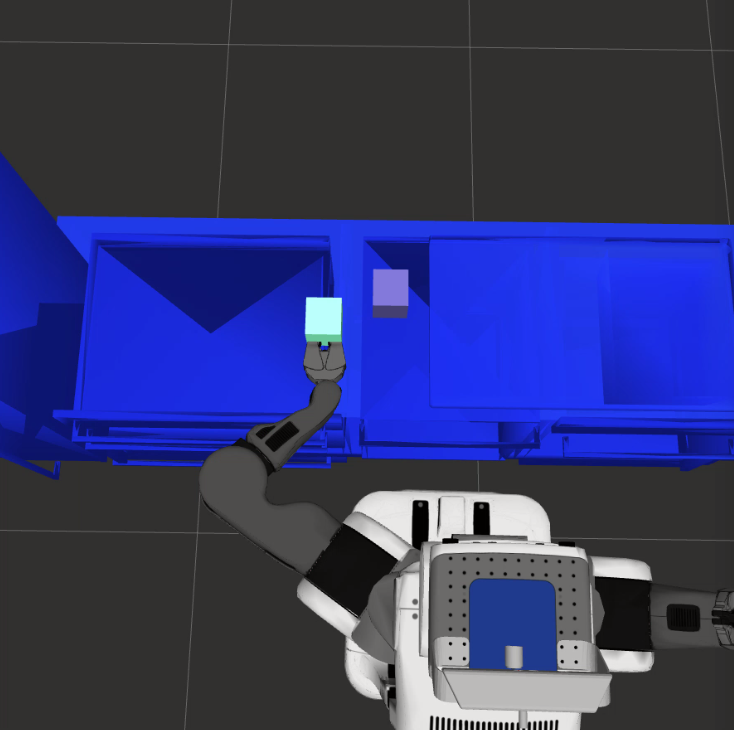
\includegraphics[width=1.0\textwidth]
		{img/objects_push.png}
		\caption{} Das Verschieben von Objekten}
\end{figure}

\subsubsection{calculate-landing-zone-visualized()}
\chapterauthor{Hauke Tietjen}
\begin{verbatim}
calculate-landing-zone-visualized()

Beschreibung: Die Funktion führt calculate-landing-zone() aus und
visualisiert das Ergebnis, mit visualize-landing-zone().

@param object
@return Gibt eine Pose in /map zurück um ein Objekt zu greifen
\end{verbatim}

\subsubsection{visualize-landing-zone()}
\chapterauthor{Hauke Tietjen}
\begin{verbatim}
visualize-landing-zone()

Beschreibung: Die Funktion führt vis-init() und publish-pose() aus
um eine Pose zu visualisieren.

@param pose
@return 
\end{verbatim}

\subsubsection{vis-init()}
\chapterauthor{Hauke Tietjen}
\begin{verbatim}
vis-init()

Beschreibung: Die Funktion startet den Marker-publisher.

@param 
@return 
\end{verbatim}

\subsubsection{publish-pose()}
\chapterauthor{Hauke Tietjen}
\begin{verbatim}
publish-pose()

Beschreibung: Es wird ein Marker an der angegebenen Pose publiziert,
mit ID und den Dimensionen aus height und width. Der Marker hat die
Form eines Würfels und die Farbe wird zufällig gewählt.

@param pose id height width
@return 
\end{verbatim}

\section{Die Quellcode-Datei: error-hierarchy.lisp (planning\_error)}
\subsection{Architekturbild}
\chapterauthor{Hauke Tietjen}
\begin{figure}[!htb]
	\center{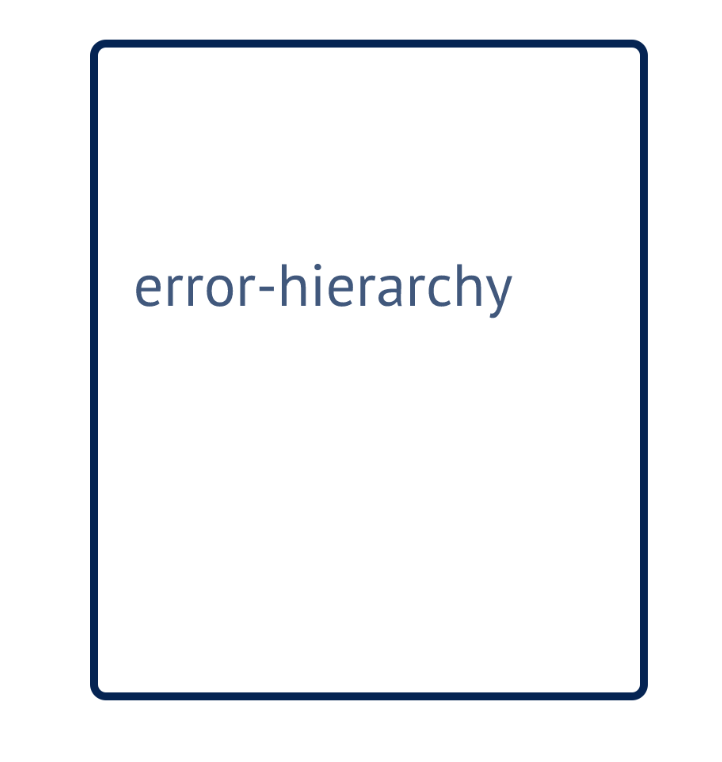
\includegraphics[width=0.4\textwidth]
		{img/diag_planning_error.png}
		\caption{} Architektur der Quellcode-Datei error-hierarchy.lisp}
\end{figure}


\subsection{API}
\chapterauthor{Hauke Tietjen}
\subsubsection{Serviceclients}
keine
\subsection{Beschreibung des Teilsystems}
\subsubsection{\"Ubersicht}
\chapterauthor{Hauke Tietjen}
Die Datei 'error-hierarchy' aus dem Paket 'planning\_error' legt die Hierarchie der Fehler fest.

\begin{figure}[!htb]
	\center{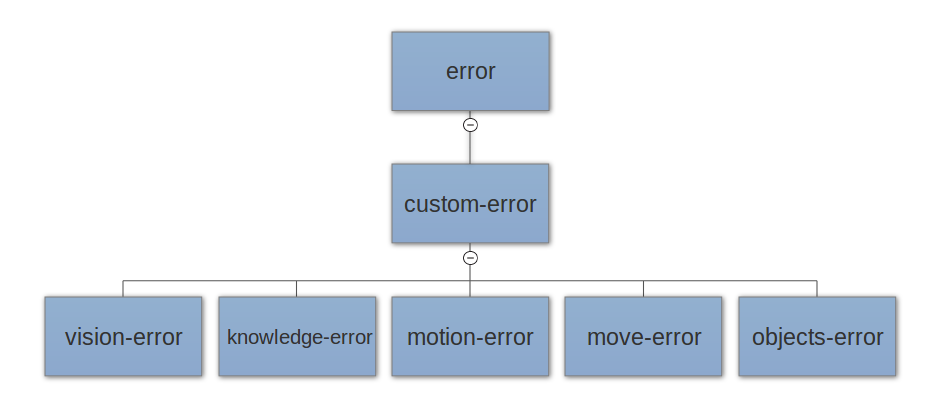
\includegraphics[width=1.0\textwidth]
		{img/error_hierarchy.png}
		\caption{} Fehlerhierarchie}
\end{figure}

\subsubsection{custom-error()}
\chapterauthor{Hauke Tietjen}
\begin{verbatim}
custom-error()

Beschreibung: Dieser Standardfehler erbt von 'error' während
alle weiteren Fehler von diesem erben. 

@param message
@return 
\end{verbatim}

\subsubsection{vision-error()}
\chapterauthor{Hauke Tietjen}
\begin{verbatim}
vision-error()

Beschreibung: Diese Fehlerklasse beschreibt Fehler, die im
Zusammenhang mit Vision stehen. Vor der 
Fehlernachricht wird 'vison error:' ausgegeben. 

@param
@return 
\end{verbatim}

Die Conditions 'motion-error', 'move-error', 'knowledge-error' und 'objects-error' funktionieren analog zu 'vison-error' und definieren weitere Fehler, für andere Bereiche.
\section{Die Quellcode-Datei: interaction.lisp (planning\_interaction)}
\subsection{Architekturbild}
\chapterauthor{Kevin Störmer}



\begin{figure}[!htb]
	\center{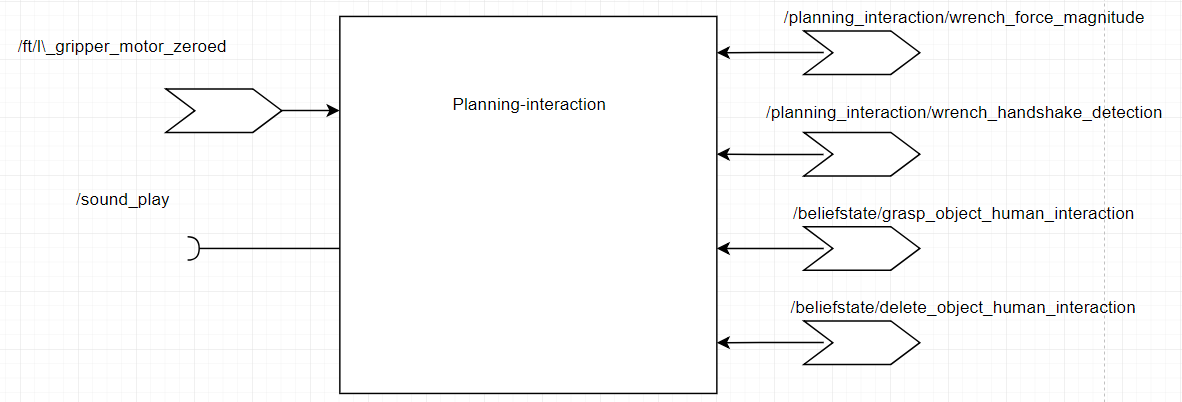
\includegraphics[width=1.0\textwidth]
		{img/diag_planning_interaction.png}
		\caption{} Architektur der Quellcode-Datei planning-interaction.lisp}
\end{figure}



\subsection{API}
\chapterauthor{Kevin Störmmer}
\subsubsection{Topics}
1. '/planning\_interaction/wrench\_force\_magnitude' \\
Published auf dem Topic den Betrag des Kraeftevektors des Handgelenkes.\\ \\
2. '/planning\_interaction/wrench\_handshake\_detection' \\
Published auf dem Topic eine 15 wenn Ein Handshake wahrgenommen wird.\\ \\
3. '/beliefstate/grasp\_object\_human\_interaction' \\
Published für Knowledge eine Message, wenn ein Objekt von einem Menschen in den Gripper gelegt wird.\\ \\
4. '/beliefstate/delete\_object\_human\_interaction' \\
Published für Knowledge eine Message wenn ein Objekt aus dem Gripper des Pr2 entfernt wird.\\ \\
5. '/ft/l\_gripper\_motor\_zeroed' \\
Subscribed auf den Topic um die kalibrierten Handgelenkswerte des Pr2 zu bekommen.\\ \\
\subsubsection{Actionserver}
1. '/sound\_play' \\
Nutzt die Soundplay Action, des Sound\_Play Paketes um dem Pr2 eine Stimme zu synthetisieren.\\ \\
\subsection{Beschreibung des Teilsystems}
\subsubsection{\"Ubersicht}
\chapterauthor{Kevin Störmer}
Die Datei interaction.lisp ist zuständig dafür, Situationen aufzuloesen, die nicht vom Code abgedeckt werden, oder die für den Roboter physikalisch nicht möglich sind.\\
Dabei soll vorallem auf Sicherheit der Interaktion und Einfachheit in der Implementation geachtet werden. Fokus liegt dabei auch auf dem Feststellen von Handshake-Actions sodass dem Menschen eine Interaktionsschnittstelle gegeben wird.\\
Wie in der folgenden Illustration gezeigt, werden Sicherheitskritische Aspekte dabei von den oeffentlichen Funktionen getrennt.
\begin{figure}[!htb]
	\center{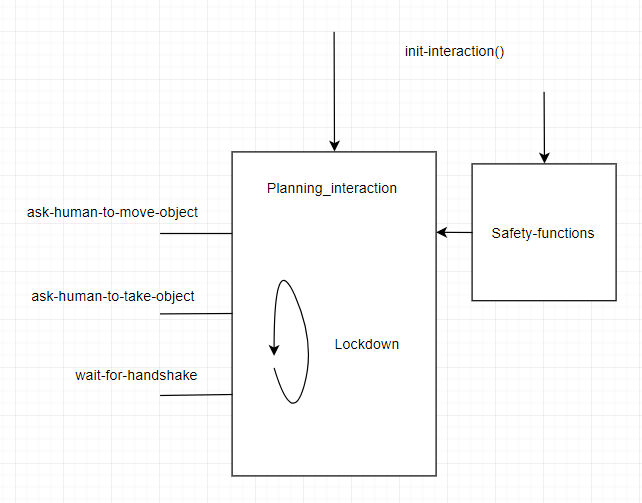
\includegraphics[width=1.0\textwidth]
		{img/ablauf_planning_interaction.png}
		\caption{} Ablauf der Initialisierung}
\end{figure}

\subsubsection{init-interaction()}
\chapterauthor{Kevin Störmer}
\begin{verbatim}
init-interaction()
Beschreibung: Initialisiert das Paket. Startet alle Subkomponenten, 
und teilt dem Nutzer mit falls Abhängigkeiten fehlen.
@return true wenn richtig initalisiert
\end{verbatim}

\subsubsection{ask-human-to-move-object()}
\chapterauthor{Kevin Störmer}
\begin{verbatim}
ask-human-to-move-object()
Beschreibung: Fehlerfallabdeckung für den Fall das der Pr2 ein Objekt
nicht greifen kann. Pr2 zeigt dann auf das Objekt, und ruft 
einen Menschen zu Hilfe.
Dieser kann dann das Objekt in den Gripper des Pr2 legen 
und ihm die Hand schütteln. Der Roboter nimmt dann seine Arbeit 
wieder auf.
@param pose label force moving command statement1 statement2
@return Kein definierter Rückgabewert
\end{verbatim}

\subsubsection{ask-human-to-take-object ()}
\chapterauthor{Kevin Störmer}
\begin{verbatim}
ask-human-to-take-object ()
Beschreibung: Fehlerfallabdeckung für den Fall das der Pr2 ein Objekt 
nicht ablegen kann. Der Pr2 fährt dann an einen Ort an dem er gut 
mit dem Menschen interagieren kann. Dort streckt er seine Arme aus 
und verweist auf den Gripper in dem das Objekt steckt, 
welches er loswerden möchte. \\
Nach einem Händeschütteln, wird das Objekt freigegeben 
und als abgelegt behandelt. Der PR2 nimmt dann seine Arbeit wieder auf.
@param label moving-command
@return Kein definierter Rückgabewert
\end{verbatim}

\subsubsection{check-gripper()}
\chapterauthor{Kevin Störmer}
\begin{verbatim}
check-gripper()
Beschreibung: Anpassbare Funktion für beliebige Fehlerfälle. Es kann 
eine Funktion übergeben werden, welche dann in einer sicheren 
Umgebung aufgerufen wird. Nebenbei werden die beiden Gripper gecheckt, 
sodass nichts aus dem Gripper fallen kann währenddessen. Wenn kein 
Fehlschlag passiert, läuft die mitgegebene Funktion normal durch.
@param errormsg func args r l)
@return Kein definierter Rückgabewert
\end{verbatim}

\subsubsection{decide-gripper()}
\chapterauthor{Kevin Störmer}
\begin{verbatim}
decide-gripper()
Beschreibung: Da Motion merkwürdige Magic-Numbers für ihre Actions verwendet, 
wird diese Funktion gebraucht um von der Einen auf die Andere schliessen zu 
können.
@param moving-command
@return magic-number für die Gripper-Action
\end{verbatim}

\subsubsection{drive-to-human ()}
\chapterauthor{Kevin Störmer}
\begin{verbatim}
drive-to-human ()
Beschreibung: Fährt zu Ort für menschliche Interaction an der Iai Holz-Küche.
@param -
@return Kein definierter Rückgabewert
\end{verbatim}

\subsubsection{say ()}
\chapterauthor{Kevin Störmer}
\begin{verbatim}
say ()
Beschreibung: Nutzt das sound\_play Paket um einen String in 
gesprochene Sprache zu synthetisieren und auf dem Pr2 auszugeben.
@param message
@return Kein definierter Rückgabewert
\end{verbatim}

\subsubsection{wait-for-handshake ()}
\chapterauthor{Kevin Störmer}
\begin{verbatim}
wait-for-handshake ()
Beschreibung: Anpassbare Funktion zur Konfiguration eigener Fehlerfälle. 
Pr2 führt stoppt seine Aufgabe, und gibt mitgegebene Errormessage aus. 
Danach wartet er auf einen Handshake und führt dann die mitgegebene 
Funktion aus.
@param func args errormsg
@return Kein definierter Rückgabewert
\end{verbatim}

\subsubsection{build-pointing-pose ()}
\chapterauthor{Kevin Störmer}
\begin{verbatim}
build-pointing-pose ()
Beschreibung: Baut die Pointing-Pose aus den einzelnen Berechnungen 
zusammen. Diese Pose wird gebraucht um auf ein Objekt zu zeigen.
@param pose
@return Pose die auf das Objekt zeigt
\end{verbatim}

\subsubsection{get-pointing-pose ()}
\chapterauthor{Kevin Störmer}
\begin{verbatim}
get-pointing-pose ()
Beschreibung: Baut die Pointing-Pose zusammen, ohne Quaternion. 
Verarbeitet die Daten aus 'get-vektor-pr2-reachable' 
(beschrieben nachfolgend). 
@param pose
@return Pointing-Pose ohne Quaternion
\end{verbatim}

\subsubsection{get-vektor-pr2-reachable ()}
\chapterauthor{Kevin Störmer}
\begin{verbatim}
get-vektor-pr2-reachable ()
Beschreibung: Rechnet in Abhängigkeit von Arm und Gegebenem 
Vektor den nähesten Punkt aus den der Pr2 erreichen kann
@param vektor
@return erreichbarer Punkt
\end{verbatim}

\subsubsection{calculate-pointing-quaternion ()}
\chapterauthor{Kevin Störmer}
\begin{verbatim}
calculate-pointing-quaternion ()
Beschreibung: Berechnet aus einer gegebenen Object-Pose das 
Quaternion was benötigt wird um auf ein Objekt zu zeigen. 
@param object-pos
@return quaternion, welches zum pointen gebraucht wird
\end{verbatim}

\subsubsection{get-directional-vector ()}
\chapterauthor{Kevin Störmer}
\begin{verbatim}
get-directional-vector ()
Beschreibung: Berechnet aus 2 Punkten im Raum den Richtungsvektor in Richtung 
des 2ten Punktes.
@param Vektor1 Vektor2
@return Richtungsvektor
\end{verbatim}

\subsubsection{vectors-to-matrix ()}
\chapterauthor{Kevin Störmer}
\begin{verbatim}
vectors-to-matrix ()
Beschreibung: Baut und berechnet aus 3 Punkten oder Vektoren im Raum eine 
Transformationsmatrix.
@param Vektor-x Vector-y Vector-z
@return 3x3 Tansformationsmatrix
\end{verbatim}

\newpage

\subsubsection{calculate-wrench-magnitude ()}
\chapterauthor{Kevin Störmer}
\begin{verbatim}
calculate-wrench-magnitude ()
Beschreibung: Berechnet Betrag der Wrench-Force-Daten und published sie. 
Ausserdem wird immer genau dann auf dem Handshake-detection gepublished, 
wenn ein Handschlag festgestellt wird. (Callback-Funktion)
@param msg
@return Kein definierter Rückgabewert
\end{verbatim}

\begin{figure}[!htb]
	\center{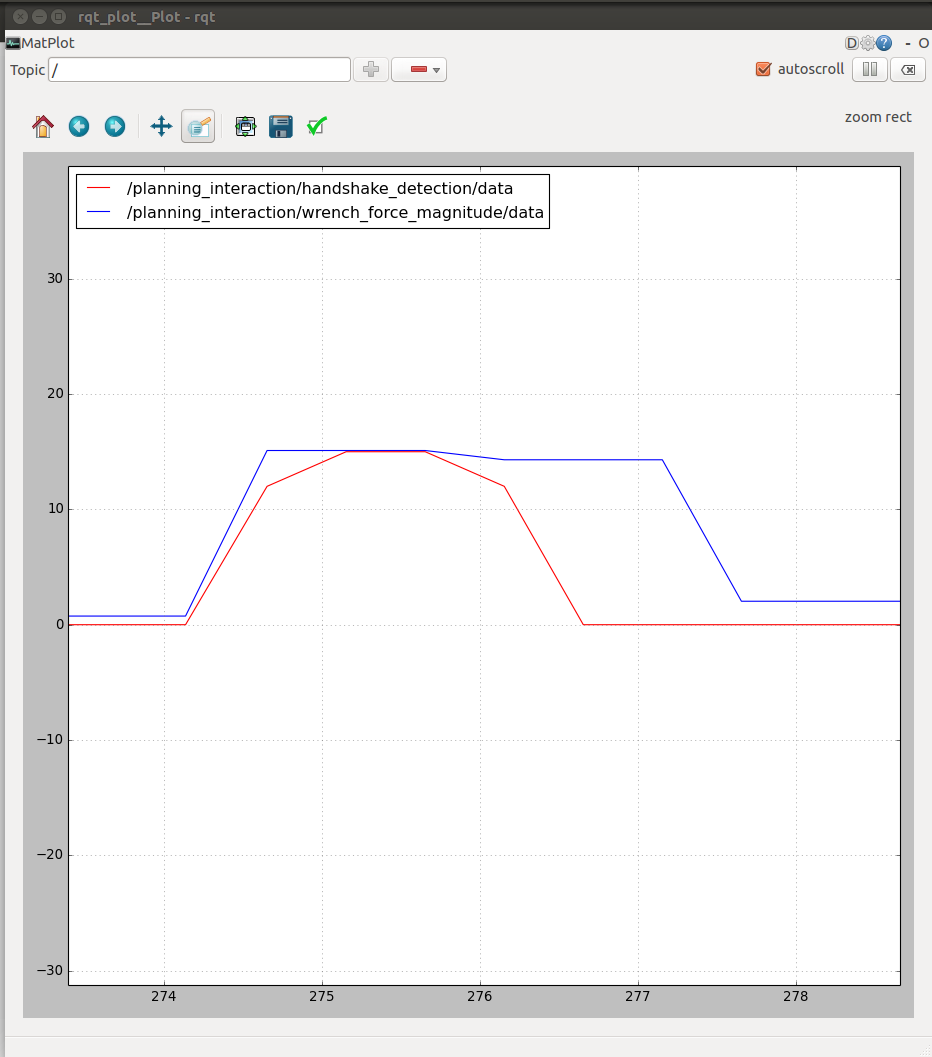
\includegraphics[width=1.0\textwidth]
		{img/detection_planning_interaction.png}
		\caption{} Detection eines Handshakes, wie in calculate-wrench-magnitude}
\end{figure}


\subsubsection{put-object-in-hand ()}
\chapterauthor{Kevin Störmer}
\begin{verbatim}
put-object-in-hand ()
Beschreibung: Simple Methode um Knowledge mitzuteilen, wenn ein Objekt 
in den Gripper gelegt wird.
@param gripper label
@return Kein definierter Rückgabewert
\end{verbatim}

\subsubsection{drop-object-in-hand ()}
\chapterauthor{Kevin Störmer}
\begin{verbatim}
drop-object-in-hand ()
Beschreibung: Simple Methode um Knowledge mitzuteilen, wenn ein Objekt 
aus dem Gripper gelegt wird.
@param label
@return Kein definierter Rückgabewert
\end{verbatim}

\newpage

\section{Die Quellcode-Datei: old.lisp (planning\_old)}

\subsubsection{disassemble-Vision-Call (visionclouds)}
\chapterauthor{Vanessa Hassouna}
\begin{verbatim}
disassemble-Vision-Call (visionclouds)

Beschreibung: Extrahiert alle Informationen aus der 
Visioncloud und speichert normal_features, color_features, 
object_amount und object_pose auf dem Parameterserver.
 
@param: visionclouds
@return: object_pose
\end{verbatim}



\subsubsection{set-Params-Features \\
(normal-s color-s normal-e color-e amount)}
\chapterauthor{Vanessa Hassouna}
\begin{verbatim}
set-Params-Features (normal-s color-s normal-e color-e amount)

Beschreibung: Eine Hilfsfunktion für die Funktion disassemble-Vision-Call, 
um aus normal_features und color_features konkateniert ein features-X zu 
erstellen. (Knowledge benötigt ein Array in dem zuerst color_features 
vorkommen und direkt im Anschluss normal_features)

@param: normal-s color-s normal-e color-e amount
@return: Nil
\end{verbatim}













\newpage
\section*{Methodendokumentation Gruppe Knowledge}
\section{knowledge\_grasp}
\chapterauthor{Max-Phillip Bahr}
Das Knowledge\_Grasp-Paket dient dazu, alle GraspPosen zu einem erkannten Gegenstand aus der Ontologie auszulesen. Die GraspPose dient dazu dem PR2 mitzuteilen wie ein Gegenstand zu greifen ist.

\begin{figure}[!htb]
        \center{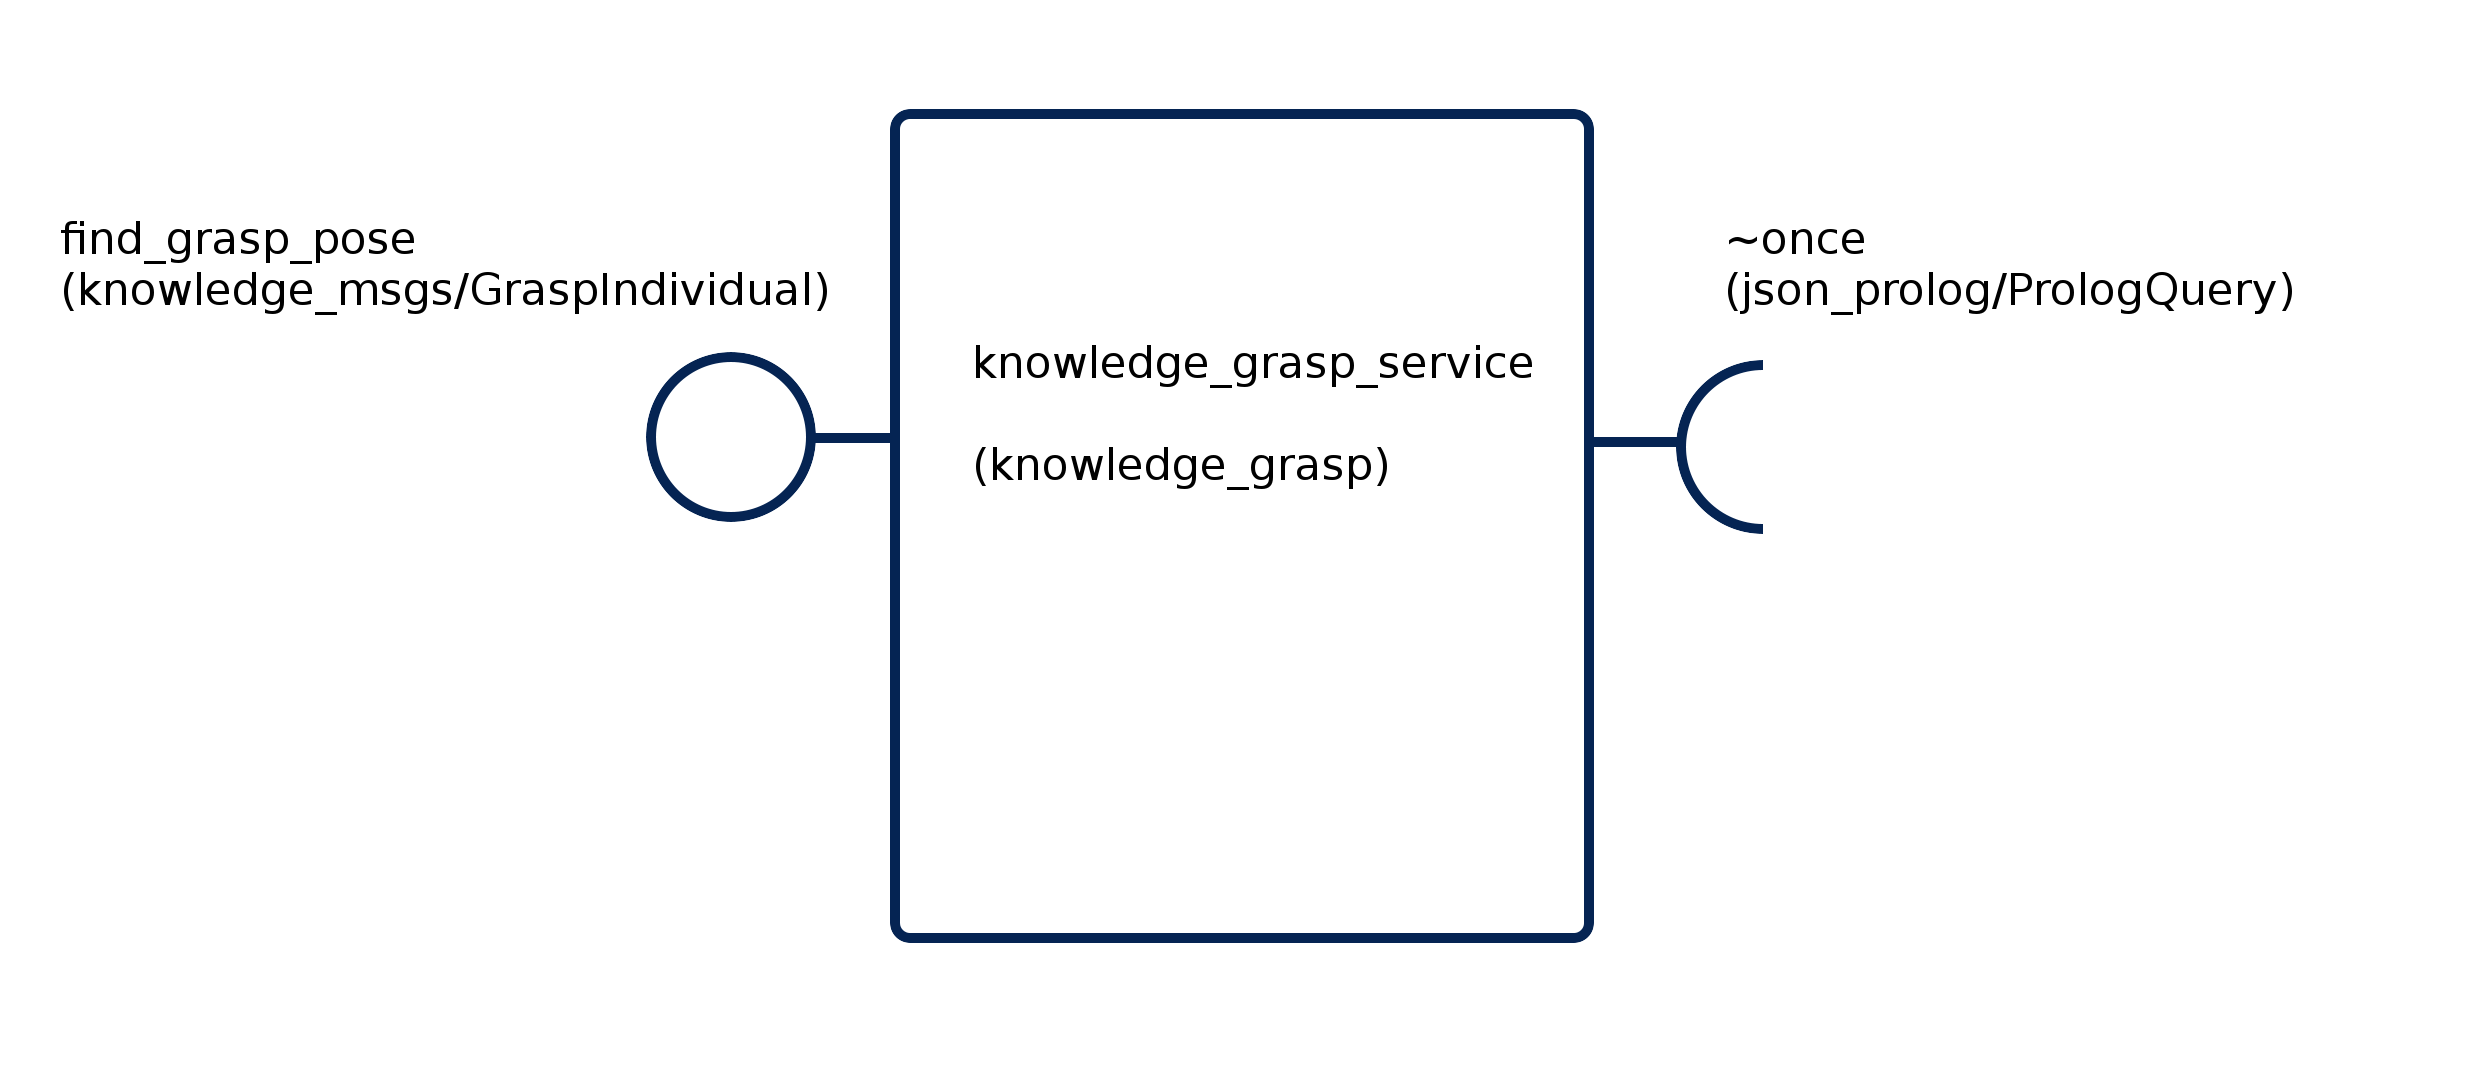
\includegraphics[width=\textwidth]
        {figures/knowledge_grasp_architektur.png}
        \caption{\label{fig:knowledge_grasp_service_node} Architektur der knowledge\_grasp\_service-node}}
\end{figure}
      
\subsection{Beschreibung des Teilsystems}
\chapterauthor{Max-Phillip Bahr}

\subsubsection*{find\_grasp\_pose - Prolog}
\begin{spverbatim}
find_grasp_pose(ObjectClassLabel, Frame, Translation, Quaternion)
@param ObjectClassLabel Das Objektlabel des zu greifenden Objekts 
       (z.B. suturo_object:'JaMilch')
@param Frame Der Frame des zu greifenden Objekts (z.B. "/JaMilch")
@param Translation Position der GraspPose als Prolog Liste 
       (z.B. [0.0, 0.0, 0.0])
@param Quaternion Orientation der GraspPose also Prolog Liste 
       (z.B. [0.0 0.0 0.0 1.0])

Description : Benutzt sort_grasp_poses um eine sortierte Liste aller 
GraspPosen zu erhalten und führt dann mit member alle Posen einzeln auf.
\end{spverbatim}

\subsubsection*{find\_grasp\_individual - Prolog}
\begin{spverbatim}
find_grasp_individual(ObjectClassLabel, GraspIndividual)
@param ObjectClassLabel Das Objektlabel des zu greifenden Objekts 
       (z.B. suturo_object:'JaMilch')
@param GraspIndividual Das zum Label gehörige Individual das 
       eine GraspPose enthält

Description : Findet alle zum einem ObjectLabel gehörigen Individuals die 
GraspPosen darstellen.
\end{spverbatim}

\subsubsection*{build\_grasp\_tuple - Prolog}
\begin{spverbatim}
build_grasp_tuple([GraspIndividual, ObjectClassLabel, Frame], 
                  [GraspIndividual, ObjectClassLabel, Frame, 
                  Translation, Quaternion])
@param GraspIndividual Das Individual der GraspPose
@param ObjectClassLabel Das zur GraspPose gehörige Objektlabel
@param Frame Der Frame des Objekts
@param Translation Die ausgelesene Position der GraspPose
@param Quaternion Die ausgelesene Rotation der GraspPose

Description : Liest die Daten aus GraspIndividual aus und fügt sie dem 
Tupel hinzu.
\end{spverbatim}

\subsubsection*{build\_pose\_list - Prolog}
\begin{spverbatim}
build_pose_list(ObjectClassLabel, Frame, PoseList)
@param ObjectClassLabel Das zur GraspPose gehörige Objektlabel
@param Frame Der Frame des Objekts
@param List Die fertige Liste von GraspPosen.

Description : benutzt findall um alle GraspIndividuals zum Objektlabel zu 
finden und dann build_grasp_tuple um die Daten der Posen den 
Tupeln in der Liste hinzuzufügen
\end{spverbatim}

\subsubsection*{evaluate\_pose\_by\_height - Prolog}
\begin{spverbatim}
evaluate_pose_by_height([Individual, Class, Frame, Translation, Quaternion], 
                        K-[Individual, Translation, Quaternion])
@param Individual Das Individual der GraspPose
@param Class Das zur GraspPose gehörige Objektlabel
@param Frame Der Frame des Objekts
@param Translation Die ausgelesene Position der GraspPose
@param Quaternion Die ausgelesene Rotation der GraspPose
@param K Dem Tupel zugeteilter Schlüsselwert

Description : Wertet die GraspPosen nach Höhenunterschied zum Ablageplatz aus 
und weist ihnen Keys zu die zum sortieren benutzt werden.
\end{spverbatim}

\subsubsection*{pair\_value - Prolog}
\begin{spverbatim}
pair_value(_-V, V)
@param V Wert eines Schlüssel-Wert Paares

Description : Entfernt den Schlüssel eines Schlüssel-Wert Paares.
\end{spverbatim}

\subsubsection*{sort\_grasp\_poses - Prolog}
\begin{spverbatim}
sort_pose_list(ObjectClassLabel, Frame, PoseList)
@param ObjectClassLabel Das Label des zu greifenden Objekts
@param Frame Der Frame des Objekts
@param SortedGraspList Die fertige Liste von GraspPosen.

Description : Baut mit build_pose_list eine Liste aus GraspPosen und weist 
ihnen mit evaluate_pose_by_height Schlüssel zu, dann werden die Posen nach 
diesen Schlüsseln sortiert und die Schlüssel danach mit pair_value aus den 
Paaren entfernt. Das Ergebnis ist eine sortierte Liste aus GraspPosen.
\end{spverbatim}

\subsubsection*{createQuery - C++}
\begin{spverbatim}
std::string createQuery(std::string object_label, std::string frame_id)
@param object_label Das Objektlabel.
@param frame_id Die ID des Objektframes.
@return Den aus dem Objektlabel und FrameID zusammengesetzten Query-String.

Description : Baut aus dem Objektlabel und der Frame ID einen Query-String 
für die Prolog-Methode find_grasp_pose zusammen.
\end{spverbatim}

\subsubsection*{find\_grasp\_pose - C++}
\begin{spverbatim}
bool find_grasp_pose(knowledge_msgs::GraspIndividual::Request  &req, 
                             knowledge_msgs::GraspIndividual::Response &res)
@param req Adresse des Request Objekts von GraspIndividual das bearbeitet 
           werden soll.
@param res Adresse zum schreiben des Response Objekts von GraspIndividual.
@return true wenn Methode erfolgreich, false wenn nicht.

Description : Die Methode liest das Objektlabel aus req aus und baut mit 
createQuery einen QueryString, der mit der query-Methode an den Prolog Server 
geschickt wird. Alle von Prolog gefundenen Lösungen werden dem PoseArray 
hinzugefügt und je nach Objektlabel die Greifstärke eingestellt
\end{spverbatim}

\subsection{Schnittstellen}
\chapterauthor{Max-Phillip Bahr}

\subsubsection{Service Server knowledge\_grasp\_service/knowledge\_grasp}
\begin{spverbatim}
GraspIndividual.srv
@request:

	string object_label

@response: 

	geometry_msgs/PoseArray grasp_pose_array
	float64 force
\end{spverbatim}
Wir entnehmen der Message das Objektlabel und lesen die für dieses Objekt gespeicherte GraspPosen aus der Ontologie aus. Die Posen werden als grasp\_pose\_array zurückgegeben.

\subsection{Programmablauf}
\chapterauthor{Max-Phillip Bahr}
\begin{itemize}
\item[1.]Es wird eine Anfrage an den Service-Server gestellt
\item[2.]Eine Anfrage mit folgendem Inhalt wird an den json\_prolog- Server wird gestellt:\\ "find\_grasp\_pose(suturo\_object:'object\_label', 'frame\_id', Position, Quaternion)." 
\item[3.]Die entsprechende Prolog Methode liest die zum übergebenen Objektlabel gehörigen GraspPosen aus der OWL Ontologie aus.
\item[4.] Die als PrologBindings vom json\_prolog- Server erhaltenen GraspPosen werden von find\_grasp\_pose (c++) in die gewünschte Form konvertiert.
\item[5.] Antwort zurückgeben.
\end{itemize}

\section{beliefstate}
\chapterauthor{Alexander Haar}
Das beliefstate-Paket dient dazu sich Aktionen die der Roboter ausgeführt hat zu speichern und auf Anfrage zu ermitteln, welcher Gripper belegt ist und welche Objekte als nächstes weggeräumt werden sollen. Außerdem spawnt der Knoten die Objektkoordinatensysteme und spawnt außerdem das Mesh des Objekts.\\
Des weiteren ist der beliefstate in die Mensch-Roboter-Interaktion involviert. Falls ein Objekt nicht gegriffen werden kann, dann wird der beliefstate so manipuliert, dass ein Zustand hergestellt wird in dem das Objekt von oben gegriffen wurde. Sollte ein Objekt nicht abgestellt werden können, dann wird des komplett aus dem beliefstate entfernt. 

\begin{figure}[!htb]
        \center{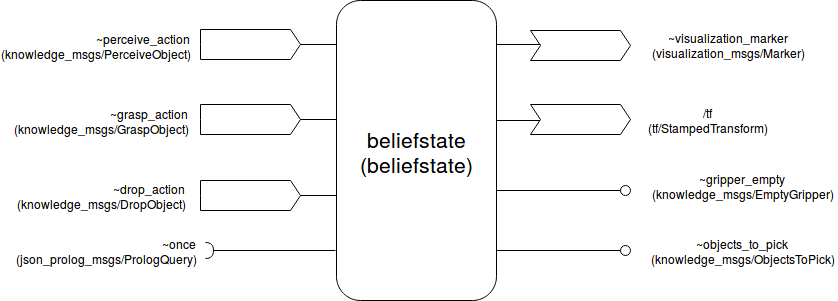
\includegraphics[width=\textwidth]
        {figures/beliefstate.png}
        \caption{\label{fig:beliefstate_node} Architektur der beliefstate-node}}
\end{figure}
      
\subsection{Beschreibung des Teilsystems}
\chapterauthor{Alexander Haar}

\subsubsection*{to\_underscore - Python}
\begin{verbatim}
def to_underscore(name)
Beschreibung: Übersetzt einen string von Camelcase- Schreibweise 
in underscore- Schreibweise. 
@param name: Der string in Camelcase- Schreibweise.
@return: Der string in underscore- Schreibweise.
\end{verbatim}

\subsubsection*{object\_url\_to\_object\_name - Python}
\begin{verbatim}
def object_url_to_object_name(url)
Beschreibung: Extrahiert aus einer Owl-Url den Namen eines Objekts.
@param url: Die Owl- Url.
@return: Der Objektname.
\end{verbatim}


\subsubsection*{prolog\_query\_false - Python}
\begin{verbatim}
def prolog_query_false(query_result)
Beschreibung: Evaluiert, ob eine Prologanfrage zu false auswertet.
@param query_result: Resultat einer einer Prologanfrage.
@return: True, falls die Prologanfrage zu false evaluiert und false sonst.
\end{verbatim}

\subsubsection*{prolog\_query\_true - Python}
\begin{verbatim}
def prolog_query_true(query_result)
Beschreibung: Evaluiert, ob eine Prologanfrage zu true auswertet.
@param query_result: Resultat einer einer Prologanfrage.
@return: True, falls die Prologanfrage zu true evaluiert und false sonst.
\end{verbatim}

\subsubsection*{point\_to\_prolog\_list - Python}
\begin{verbatim}
def point_to_prolog_list(point)
Beschreibung: Übersetzt einen Punkt in eine Prologliste.
@param point: Der zu übersetzende Punkt.
@return: Die resultierende Prologliste.
\end{verbatim}

\subsubsection*{pose\_to\_prolog\_list - Python}
\begin{verbatim}
def pose_to_prolog_list(pose)
Beschreibung: Übersetzt eine Pose in eine Prologliste.
@param pose: Die zu übersetzende Pose.
@return: Die resultierende Prologliste.
\end{verbatim}

\subsubsection*{gripper\_as\_string - Python}
\begin{verbatim}
def gripper_as_string(gripper)
Beschreibung: Übersetzt eine Gripperkonstante in einen string.
@param gripper: Die zu übersetzende Gripperkonstante.
@return: Der resultierende string.
\end{verbatim}

\subsubsection*{create\_query\_for\_perceive\_object - Python}
\begin{verbatim}
def create_query_for_perceive_object(perceive_object_msg)
Beschreibung: Erzeugt anhand einer PerceiveObject.msg eine Prologanfrage.
@param perceive_object_msg: Die PerceiveObject.msg.
@return: Die resultierende Prologanfrage.
\end{verbatim}

\subsubsection*{create\_query\_for\_grasp\_object - Python}
\begin{verbatim}
def create_query_for_grasp_object(grasp_object_msg)
Beschreibung: Erzeugt anhand einer GraspObject.msg eine Prologanfrage.
@param grasp_object_msg: Die GraspObject.msg.
@return: Die resultierende Prologanfrage.
\end{verbatim}

\subsubsection*{create\_query\_for\_drop\_object - Python}
\begin{verbatim}
def create_query_for_drop_object(drop_object_msg)
Beschreibung: Erzeugt anhand einer DropObject.msg eine Prologanfrage.
@param drop_object_msg: Die DropObject.msg.
@return: Die resultierende Prologanfrage.
\end{verbatim}

\subsubsection*{create\_query\_object\_attached\_to\_gripper - Python}
\begin{verbatim}
def create_query_object_attached_to_gripper(gripper)
Beschreibung: Erzeugt anhand einer Gripperkonstante eine Prologanfrage.
@param gripper: Die Gripperkonstante.
@return: Die resultierende Prologanfrage.
\end{verbatim}

\subsubsection*{object\_exists - Python}
\begin{verbatim}
def object_exists(object_class)
Beschreibung: Evaluiert, ob ein Objekt bereits wahrgenommen wurde und in 
der Wissensbasis existiert.
@param object_class: Das zu überprüfende Objekt.
@return: True, falls das Objekt in der Wissensbasis existiert und false sonst.
\end{verbatim}

\subsubsection*{pose\_stamped\_to\_position\_tupel - Python}
\begin{verbatim}
def pose_stamped_to_position_tupel(pose_stamped)
Beschreibung: Übersetzt die Position eines PoseStamped in einen Tupel.
@param pose_stamped: Der zu übersetzende PoseStamped.
@return: Das resultierende Tupel.
\end{verbatim}

\subsubsection*{pose\_stamped\_to\_quaternion\_tupel - Python}
\begin{verbatim}
def pose_stamped_to_quaternion_tupel(pose_stamped)
Beschreibung: Übersetzt das Quaternion eines PoseStamped in ein Tupel.
@param pose_stamped: Der zu übersetzende PoseStamped.
@return: Das resultierende Tupel.
\end{verbatim}

\subsubsection*{quaternion\_to\_prolog\_list - Python}
\begin{verbatim}
def quaternion_to_prolog_list(quaternion)
Beschreibung: Übersetzt ein Quaternion in eine Prologliste.
@param quaternion: Das zu übersetzende Quaternion.
@return: Die resultierende Prologliste.
\end{verbatim}

\subsubsection*{spawn\_object\_frame - Python}
\begin{verbatim}
def spawn_object_frame(object_name, object_pose)
Beschreibung: Spawnt an der angegebenen Pose ein Objektkoordinatensystem 
und das entsprechende Mesh.
@param object_name: Der Name des Objekts.
@param object_pose: Die Pose des Objekts.
\end{verbatim}

\subsubsection*{update\_object\_frame - Python}
\begin{verbatim}
def update_object_frame(object_name, object_pose)
Beschreibung: Ändert die Pose des angegeben Objekts auf die übergebene
              Pose.
@param object_name: Der Name des Objekts.
@param object_pose: Die Pose des Objekts.
\end{verbatim}

\subsubsection*{change\_reference\_frame - Python}
\begin{verbatim}
def change_reference_frame(object_name, new_reference_frame_id)
Beschreibung: Verändert das Referenzframe des Objektkoordinatensystems 
auf das übergeben Koordinatensystem.
@param object_name: Der Name des Objekts.
@param new_reference_frame_id: Das neu Referenzkoordinatensystem.
\end{verbatim}

\subsubsection*{spawn\_object\_mesh - Python}
\begin{verbatim}
def spawn_object_mesh(object_name)
Beschreibung: Spawnt ein Mesh in dem entsprechenden Objektkoordinatensystem.
@param object_name: Der Name des Objekts.
\end{verbatim}

\subsubsection*{main - Python}
\begin{verbatim}
__name__ == '__main__
Beschreibung: Startet alle Service- Server und Subscriber die
dieser Knoten benötigt.
\end{verbatim}

\subsubsection*{object\_exists - Prolog}
\begin{verbatim}
object_exists(ObjectClass)
Beschreibung: Prüft, ob ein Individual dieser Klasse bereits in der
Wissensbasis vorhanden ist
@param ObjectClass: Die zu prüfende Objektklasse.
\end{verbatim}

\subsubsection*{process\_perceive\_action - Prolog}
\begin{verbatim}
process_perceive_action(ObjectClass, PoseList, ReferenceFrame)
Beschreibung: Fügt ein Individual der Objektklasse an der angegebenen 
Pose im Referenzframe hinzu.
@param ObjectClass: Die Klasse der hinzuzufügenden Individuals.
@param PoseList: Die Pose des Objekts als Liste.
@param ReferenceFrame: Das Referenzframe.
\end{verbatim}

\subsubsection*{process\_grasp\_action - Prolog}
\begin{verbatim}
process_grasp_action(ObjectClass, GripperIndividual)
Beschreibung: Fügt eine GraspAction zur Wissensbasis hinzu unter 
Verwendung des angegeben Grippers und der Objektklasse.
@param ObjectClass: Die Objektklasse.
@param GripperIndividual: Linker oder rechter Gripper.
\end{verbatim}

\subsubsection*{process\_drop\_action - Prolog}
\begin{verbatim}
process_drop_action(GripperIndividual)
Beschreibung: Fügt eine DropAction zur Wissensbasis hinzu unter 
Verwendung des angegeben Grippers.
@param GripperIndividual: Linker oder rechter Gripper.
\end{verbatim}

\subsubsection*{object\_attached\_to\_gripper - Prolog}
\begin{verbatim}
object_attached_to_gripper(GripperIndividual, ObjectIndividual)
Beschreibung: Prüft, ob sich ein Objekt in dem angegebenen Gripper befindet.
@param GripperIndividual: Linker oder rechter Gripper.
@param ObjectIndividual: Das Objekt, welches sich im Gripper befindet.
\end{verbatim}

\subsubsection*{get\_latest\_object\_pose - Prolog}
\begin{verbatim}
get_latest_object_pose(ObjectIndividual, PoseList)
Beschreibung: Gibt die zuletzt bekannte Pose des Objekts zurück.
@param ObjectIndividual: Das Objekt.
@param PoseList: Die Pose des Objekts.
\end{verbatim}

\subsubsection*{get\_objects\_on\_kitchen\_island\_counter - Prolog}
\begin{verbatim}
get_objects_on_kitchen_island_counter(ObjectList)
Beschreibung: Gibt eine Liste aller Objekte die noch verteilt
werden müssen zurück.
@param ObjectList: Eine Liste aller Objekte die noch verteilt werden müssen.
\end{verbatim}

\subsubsection*{get\_two\_objects\_on\_kitchen\_island\_counter\_with\_same\_storage\_place - Prolog}
\begin{verbatim}
get_two_objects_on_kitchen_island_counter_with_same_storage_place
(Object1, Object2)
Beschreibung: Gibt die zwei Objekte zurück, 
welche als nächstes verteilt werden sollen.
@param Object1: Das erste Objekt.
@param Object2: Das zweite Objekt.
\end{verbatim}

\subsection{Schnittstellen}
\chapterauthor{Alexander Haar}

\subsubsection{Subscriber process\_perceive\_action}
\begin{verbatim}
def process_perceive_action(perceive_object_msg)
Beschreibung: Erstellt anhand der Message eine Prologanfrage und
sendet diese an den json_prolog- Server. 
@param perceive_object_msg: Die PerceiveObject.msg
\end{verbatim}

\subsubsection{Subscriber process\_grasp\_action}
\begin{verbatim}
def process_grasp_action(grasp_object_msg)
Beschreibung: Erstellt anhand der Message eine Prologanfrage und
sendet diese an den json_prolog- Server. 
@param grasp_object_msg: Die GraspObject.msg
\end{verbatim}

\subsubsection{Subscriber process\_drop\_action}
\begin{verbatim}
def process_drop_action(drop_object_msg)
Beschreibung: Erstellt anhand der Message eine Prologanfrage und
sendet diese an den json_prolog- Server. 
@param drop_object_msg: Die DropObject.msg
\end{verbatim}

\subsubsection{Subscriber grasp\_object\_human\_interaction}
\begin{verbatim}
def grasp_object_human_interaction(msg)
Beschreibung: Stellt einen Zustand her, in dem Der Roboter davon
              ausgeht das angegebenen Objekt im vorgegebenen
              Gripper zu halten. 
@param msg: Die erhaltenen Nachricht.
\end{verbatim}

\subsubsection{Subscriber delete\_object\_human\_interaction}
\begin{verbatim}
def delete_object_human_interaction(msg)
Beschreibung: Löscht das angegebene Objekt aus dem gesamten 
              Kenntnisstand des Roboters.
@param msg: Die erhaltenen Nachricht.
\end{verbatim}

\subsubsection{Service Server gripper\_empty}
\begin{verbatim}
def gripper_empty(req)
Beschreibung: Die Anfrage an den Server ist leer. Zurückgegeben werden
zwei booleans, welche angeben, ob der Gripper belegt ist.
@param req: Die Anfrage an den Service.
@return: Die Antwort des Services.
\end{verbatim}

\subsubsection{Service Server object\_attached\_to\_gripper}
\begin{verbatim}
def object_attached_to_gripper(req)
Beschreibung: Die Anfrage an den Server ist leer. Zurückgegeben werden
zwei booleans, welche angeben, ob der Gripper belegt ist.
@param req: Die Anfrage an den Service.
@return: Die Antwort des Services.
\end{verbatim}

\subsubsection{Service Server object\_to\_pick}
\begin{verbatim}
def objects_to_pick(req)
Beschreibung: Gibt die zwei Objekte zurück, welche als nächstes 
              weggeräumt werden sollen.
@param req: Die Anfrage an den Service.
@return: Die Antwort des Services.
\end{verbatim}

\subsubsection{Publisher despawn\_place\_preview}
Wurde ein Objekt abgestellt, dann wird dem place\_object-Knoten über dieses Topic mitgeteilt, dass die Vorschau entfernt werden kann.

\subsubsection{Publisher spawn\_attached\_object}
Auf diesem Topic publish der beliefstate, falls ein Objekt mithilfe eines Menschen gegriffen wurde.

\subsubsection{Publisher perceived\_object\_bounding\_box}
Wenn ein Objekt wahrgenommen wurde, dann wird über dieses Topic die Pose ein und das entsprechende CAD-Model an Motion weitergereicht

\subsection{Programmablauf}
\chapterauthor{Alexander Haar}
\subsubsection{Schritt 1: Wahrnehmen mehrerer Objekte}
Es werden mehre Objekte wahrgenommen und deren Label sowie Pose wird dem beliefstate bekannt gemacht.

\subsubsection{Schritt 2: Welche zwei Objekte sollen weggeräumt werden?}
Nachdem alle zu verteilenden Objekte bekannt sind, werden möglichst zwei Objekte ausgewählt, welche den gleichen Lagerplatz besitzen.

\subsubsection{Schritt 3: Greifen eines Objekts}
Das erste der beiden Objekte wird gegriffen.

\subsubsection{Schritt 4: Greifen eines weiteren Objekts}
Anschließend wird das zweite Objekt gegriffen.

\subsubsection{Schritt 5: Abstellen des 1. Objekts}
Der Roboter fährt zum entsprechenden Lagerplatz und stellt es dort ab.

\subsubsection{Schritt 6: Anfrage welcher der Gripper belegt ist}
Nun wird geprüft, ob beide Gripper leer sind, dies ist nicht der Fall.

\subsubsection{Schritt 7: Abstellen des 2. Objekts}
Der Roboter fährt zum nächsten Lagerplatz und stellt das zweite Objekt dort ab.

\subsubsection{Schritt 8: Anfrage welcher der Gripper belegt ist}
Erneut wird geprüft, ob beide Gripper leer sind, dies ist jetzt der Fall.

\subsubsection{Schritt 9: Welche Objekte sollen weggeräumt werden?}
Nun beginnt dieser Prozess wieder bei Schritt 2.


\section{storage\_place}
\chapterauthor{Alexander Haar}
Das storage\_place-Paket dient zur Ermittlung des Lagerplatzes eines Objekts.

\begin{figure}[!htb]
        \center{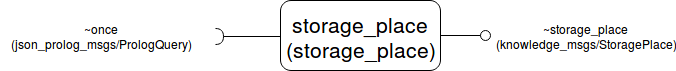
\includegraphics[width=\textwidth]
        {figures/storage_place.png}
        \caption{\label{fig:vision_node} Architektur der storage\_place-node}}
\end{figure}
      
\subsection{Beschreibung des Teilsystems}
\chapterauthor{Alexander Haar}

\subsubsection*{createQuery - C++}
\begin{verbatim}
std::string createQuery(std::string object_label)
Beschreibung: Erzeugt eine Prologanfrage, um einen Lagerplatz 
              zu ermitteln.
@param object_label: Der Name des Objekts von dem der Lagerplatz 
                     bestimmt werden soll.
\end{verbatim}

\subsubsection*{main - C++}
\begin{verbatim}
int main(int argc, char **argv)
Beschreibung: Startet den Knoten.
\end{verbatim}


\subsubsection*{get\_position - Prolog}
\begin{verbatim}
get_position(PositionIndividual, X, Y, Z)
Beschreibung: Extrahiert aus einem Position, die Koordinaten.
@param PositionIndividual: Die Position
@param X: Die X- Koordinate
@param Y: Die Y- Koordinate
@param Z: Die Z- Koordinate
\end{verbatim}

\subsubsection*{get\_scale - Prolog}
\begin{verbatim}
get_scale(StorageAreaIndividual, Width, Height)
Beschreibung: Extrahiert aus einer Lagerfläche die Ausmaße.
@param StorageAreaIndividual: Die Lagerfläche
@param Width: Die Breite der Lagerfläche
@param Height: Die Höhe der Lagerfläche
\end{verbatim}

\subsubsection*{storage\_area - Prolog}
\begin{verbatim}
storage_area(ObjectClass, StorageAreaIndividual)
Beschreibung: Ermittelt zu einer Objektklasse die Lagerfläche.
@param ObjectClass: Die Objektklasse zu der eine Lagerfläche
ermittelt werden soll.
@param StorageAreaIndividual: Die ermittelte Lagerfläche.
\end{verbatim}

\subsubsection*{storage\_place - Prolog}
\begin{verbatim}
storage_place(ObjectClass, [X, Y, Z], Width, Height)
Beschreibung: Ermittelt zu einer Objektklasse den Lagerplatz.
@param ObjectClass: Die Objektklasse zu der
ein Lagerplatz ermittelt werden soll.
@param X: Die X- Koordinate des Lagerplatzes.
@param Y: Die Y- Koordinate des Lagerplatzes.
@param Z: Die Z- Koordinate des Lagerplatzes.
@param Width: Die Breite des Lagerplatzes.
@param Height: Die Höhe des Lagerplatzes.
\end{verbatim}

\subsection{Schnittstellen}
\chapterauthor{Alexander Haar}

\subsubsection{Service Server find\_storage\_place}
\begin{verbatim}
bool find_storage_place(knowledge_msgs::StoragePlace::Request &req,
 knowledge_msgs::StoragePlace::Response &res)
Beschreibung: Service- Methode, welche einen Lagerplatz für Objekte 
              ermittelt.
@param req: Die Anfrage an den Service, welche den Namen des Objekts 
            enthält.  
@param res: Die Antwort des Services, welche das Zentrum und die 
            Ausmaße des Lagerplatzes enthält.
@return: true, falls der Aufruf erfolgreich war und false sonst.
\end{verbatim}\label{func:findcluster}

\subsection{Programmablauf}
\chapterauthor{Alexander Haar}
\subsubsection{Schritt 1: Anfrage an den Service- Server}
Eine Objektklasse wird an den Service- Server übergeben.
\subsubsection{Schritt 2: Erstellen der Prologanfrage}
Anhand der Objektklasse wird eine Prologanfrage erstellt und an den json\_prolog- Server geschickt.
\subsubsection{Schritt 3: Ermitteln des Lagerplatzes} 
Durch die oben definierten Prologregeln wird unter Verwendung von only- restrictions der Lagerplatz ermittelt.
\subsubsection{Schritt 4: Zurückgeben der Antwort}
Die vom json\_prolog- Server erhaltene Antwort wird entsprechend geparst und zurückgegeben.

\section{push\_object}
\chapterauthor{Alexander Haar}
Das push\_object-Paket errechnet einen Punkt auf der Oberfläche eines abgestellten Objektes, damit es nach hinten geschoben werden kann. Dabei wird ausgenutzt, dass die Objekte immer gleich abgestellt werden. Bei den runden Objekten ist es für schieben unerheblich wie sie abgestellt werden, bei den eckigen Objekte zeigt aber immer die kurze Seite zum Roboter. Da man die Position des Objekte im Raum kennt und die geometrischen Abmessungen kann man nun eine passende Schiebepose berechnen.

\begin{figure}[!htb]
        \center{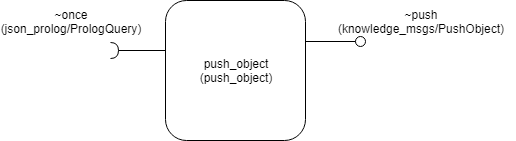
\includegraphics[width=\textwidth]
        {figures/push_object.png}
        \caption{\label{fig:push} Architektur der push\_object-node}}
\end{figure}
      
\subsection{Beschreibung des Teilsystems}
\chapterauthor{Alexander Haar}

\subsubsection*{create\_query - Python}
\begin{verbatim}
def create_query(req)
Beschreibung: Erzeugt eine Prologanfrage, um eine Schiebepose 
              zu ermitteln.
@param object_label: Der Name des Objekts, welches geschoben
                     werden soll.
\end{verbatim}


\subsubsection*{main - Python}
\begin{verbatim}
if __name__ == '__main__'
Beschreibung: Startet den Knoten.
\end{verbatim}


\subsubsection*{object\_depth - Prolog}
\begin{verbatim}
object_depth(ObjectClass, Depth)
Beschreibung: Gibt zu einer Objektklasse die entsprechende Tiefe zurück.
@param ObjectClass: Die Objektklasse zu der die Tiefe ermittelt werden soll.
@param Depth: Die Objekttiefe.
\end{verbatim}

\subsubsection*{calculate\_push\_pose - Prolog}
\begin{verbatim}
calculate_push_pose(ObjectClass, SourceFrame, X, Y, Z)
Beschreibung: Extrahiert aus einer Lagerfläche die Ausmaße.
@param ObjectClass: Die Objektklasse zu der die Schiebepose ermittelt werden soll.
@param SourceFrame: Das Frame, welches sich im Mittelpunkt des Objekts befindet.
@param X: Die X-Position der Schiebepose.
@param Y: Die Y-Position der Schiebepose.
@param Z: Die Z-Position der Schiebepose.
\end{verbatim}

\subsection{Schnittstellen}
\chapterauthor{Alexander Haar}

\subsubsection{Service Server /push\_object/push}
\begin{verbatim}
def push_object(req)
Beschreibung: Service- Methode, welche eine Schiebepose für Objekte 
              ermittelt.
@param req: Die Anfrage an den Service, welche den Namen des Objekts 
            enthält.  
@return: Die Antwort des Services, welche die Schiebepose enthält.

\end{verbatim}

\subsection{Programmablauf}
\chapterauthor{Alexander Haar}
\subsubsection{Schritt 1: Anfrage an den Service- Server}
Eine Objektklasse wird an den Service- Server übergeben.
\subsubsection{Schritt 2: Erstellen der Prologanfrage}
Anhand der Objektklasse wird eine Prologanfrage erstellt und an den json\_prolog- Server geschickt.
\subsubsection{Schritt 3: Ermitteln der Schiebepose} 
Es wird mithilfe von Prolog eine Schiebepose errechnet. Das genaue Vorgehen ist oben in den einleitenden Worten beschrieben.
\subsubsection{Schritt 4: Zurückgeben der Antwort}
Die vom json\_prolog- Server erhaltene Antwort wird entsprechend geparst und zurückgegeben.

\section{place\_object}
\chapterauthor{Alexander Haar}
Das push\_object-Paket berechnet zu einer vorgegebenen x -und y-Koordinate die passende z-Koordinate, damit ein Objekt exakt auf einem Tisch abgestellt wird. Dabei errechnet sich die z-Koordinate aus der Höhe des Tisches(0.85), die Hälfte der Objekthöhe und der Gripperposition relativ zum Mittelpunkt. Aus diesen drei Parametern lässt sich dann eine optimale z-Koordinate bestimmen. Außerdem wird beim Aufruf des Services eine Vorschau des abgestellten Objekts erstellt.

\begin{figure}[!htb]
        \center{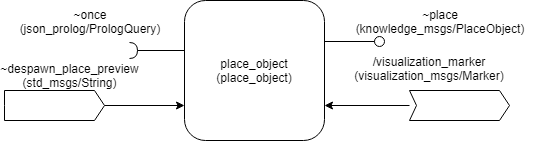
\includegraphics[width=\textwidth]
        {figures/place_object.png}
        \caption{\label{fig:place} Architektur der place\_object-node}}
\end{figure}
      
\subsection{Beschreibung des Teilsystems}
\chapterauthor{Alexander Haar}

\subsubsection*{create\_place\_query - Python}
\begin{verbatim}
def create_place_query(req)
Beschreibung: Erzeugt eine Prologanfrage, um eine passende 
              z-Koordinate zum Abstellen zu ermitteln.
@param req: Die Anfrage an den Service, welcher den Gripper 
            enthält, dessen Objekt abgestellt werden soll.
@return: Ein String, welcher die Prologanfrage enthält.
\end{verbatim}

\subsubsection*{create\_object\_height\_query - Python}
\begin{verbatim}
def create_object_height_query(object_label)
Beschreibung: Erzeugt eine Prologanfrage, um die Höhe eines Objekts zu ermitteln.
@param object_label: Der Name des Objekts, dessen Höhe ermittelt werden soll.
@return: Ein String, welcher die Prologanfrage enthält.
\end{verbatim}

\subsubsection*{spawn\_object\_mesh - Python}
\begin{verbatim}
def spawn_object_mesh(x, y, object_label)
Beschreibung: Spawn das Objekt- Mesh als Vorschau des abgestellten 
              Objekts an der vorgegeben x -und y-Position.
@param object_label: Der Name des Objekts, welches abgestellt werden soll.
\end{verbatim}

\subsubsection*{main - Python}
\begin{verbatim}
if __name__ == '__main__'
Beschreibung: Startet den Knoten.
\end{verbatim}


\subsubsection*{get\_grasp\_pose\_individual - Prolog}
\begin{verbatim}
get_grasp_pose_individual(ObjectClass, [[X,Y,Z],[QX,QY,QZ,QW]], GraspPoseIndividual)
Beschreibung: Gibt zu einer Objektklasse das GraspPoseIndividual zurück, 
              welches zum 2. Parameter passt.
@param: ObjectClass: Die Objektklasse zu der das GraspPoseIndividual 
        ermittelt werden soll.
@param: [[X,Y,Z],[QX,QY,QZ,QW]]: Die Greifpose.
@param: Das passende GraspPoseIndividual.
\end{verbatim}

\subsubsection*{object\_height - Prolog}
\begin{verbatim}
object_height(ObjectClass, Height)
Beschreibung: Gibt zu einer Objektklasse die entsprechende Höhe zurück.
@param ObjectClass: Die Objektklasse zu der die Höhe ermittelt werden soll.
@param Height: Die Objekthöhe.
\end{verbatim}

\subsubsection*{calculate\_place\_pose - Prolog}
\begin{verbatim}
calculate_place_pose(GripperIndividual, Z, [QX, QY, QZ, QW])
Beschreibung:Berechnet zum Objekt, welches sich im angegebenen Gripper
             befindet eine passende Rotation und z-Koordinate 
             zum Abstellen.
@param GripperIndividual: Der Gripper in dem Sich das Objekt befindet.
@param Z: Die z-Koordinate des Grippers beim Abstellen.
@param [QX, QY, QZ, QW]: Die Rotation des Grippers beim Abstellen.
\end{verbatim}

\subsection{Schnittstellen}
\chapterauthor{Alexander Haar}

\subsubsection{Service Server /place\_object/place}
\begin{verbatim}
def place_object(req)
Beschreibung: Service- Methode, welche eine Abstellpose für Objekte 
              ermittelt.
@param req: Die Anfrage an den Service, welche den Gripper in dem 
            sich das Objekt befindet enthält.  
@return: Die Antwort des Services, welche die Abstellpose enthält.

\end{verbatim}

\subsubsection{Subscriber /place\_object/despawn\_place\_preview}
\begin{verbatim}
def despawn_object_mesh(object_label)
Beschreibung: Diese Methode lässt die Vorschau des 
              abzustellenden Objekts wieder despawnen.
@param object_label: Der Name des Objekts.

\end{verbatim}

\subsection{Programmablauf}
\chapterauthor{Alexander Haar}
\subsubsection{Schritt 1: Anfrage an den Service- Server}
Ein Gripper wird an den Service- Server übergeben.
\subsubsection{Schritt 2: Erstellen der Prologanfrage}
Anhand des Grippers wird eine Prologanfrage erstellt und an den json\_prolog- Server geschickt.
\subsubsection{Schritt 3: Ermitteln der Abstellpose} 
Es wird mithilfe von Prolog eine Abstellpose errechnet. Das genaue Vorgehen ist oben in den einleitenden Worten beschrieben.
\subsubsection{Schritt 4: Zurückgeben der Antwort}
Die vom json\_prolog- Server erhaltene Antwort wird entsprechend geparst und zurückgegeben.
\subsubsection{Schritt 5: Spawnen der Vorschau} 
Es wird anschließend das Objekt-Mesh gespawn, so wie das Objekt perfekt abgestellt aussehen sollte.

\section{kitchen\_model\_export}
\chapterauthor{Alexander Haar}
Das Kitchen\_Model\_Export-Paket dient dazu der Manipulation die Umgebung bekannt zu machen, damit der PR2 nicht mit der Umgebung kollidiert.

\begin{figure}[!htb]
        \center{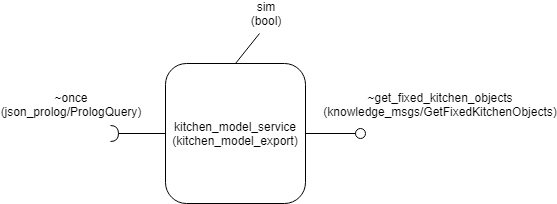
\includegraphics[width=\textwidth]
        {figures/kitchen_model_export.png}
        \caption{\label{fig:kitchen} Architektur der kitchen\_model\_export-node}}
\end{figure}
      
\subsection{Beschreibung des Teilsystems}
\chapterauthor{Alexander Haar}

\subsubsection*{main - C++}
\begin{verbatim}
int main(int argc, char **argv)
Beschreibung: Startet den Knoten und liest den Parameter sim ein.
\end{verbatim}

\subsubsection*{path\_to\_cad\_model - Prolog}
\begin{verbatim}
path_to_cad_model(IAIKitchenObjectClass, Path)
Beschreibung: Ermittel zu einem Küchenobjekt den CAD-Model-Pfad.
@param IAIKitchenObjectClass: Die Küchenobjektklasse
@param Path: Der Pfad zum CAD-Model des Küchenobjekts.
\end{verbatim}

\subsubsection*{get\_frame - Prolog}
\begin{verbatim}
get_frame(KitchenObjectIndividual, Frame)
Beschreibung: Gibt zu einem Küchenobjekt den Frame in dem es 
              sich befindet zurück.
@param KitchenObjectIndividual: Das Küchenobjekt.
@param Frame: Der Frame in dem sich das Objekt befindet.
\end{verbatim}

\subsubsection*{get\_frame\_without\_prefix - Prolog}
\begin{verbatim}
get_frame_without_prefix(KitchenObjectIndividual, Frame)
Beschreibung: Gibt zu einem Küchenobjekt den Frame in dem es 
              sich befindet ohne Prefix zurück.
@param KitchenObjectIndividual: Das Küchenobjekt.
@param Frame: Der Frame in dem sich das Objekt befindet ohne Prefix.
\end{verbatim}

\subsubsection*{is\_iai\_kitchen\_object - Prolog}
\begin{verbatim}
is_iai_kitchen_object(IAIKitchenObjectClass)
Beschreibung: Bestimmt, ob es sich bei einem Objekt um ein 
              Küchenobjekt handelt.
@param: IAIKitchenObjectClass: Das zu prüfende Objekt.
\end{verbatim}

\subsubsection*{get\_fixed\_kitchen\_objects - Prolog}
\begin{verbatim}
get_fixed_kitchen_objects(ObjectIndividual, Path, Frame)
Beschreibung: Ermittelt alle Küchenobjekte, sowie deren 
              CAD-Model-Pfad und entsprechendem Frame.
@param ObjectIndividual: Das Küchenobjekt.
@param Path: Der Pfad des CAD-Model.
@param Frame: Der Frame des Küchenobjekts.
\end{verbatim}

\subsubsection*{get\_fixed\_kitchen\_objects\_without\_prefix - Prolog}
\begin{verbatim}
get_fixed_kitchen_objects_without_prefix(ObjectIndividual, Path, Frame) 
Beschreibung: Ermittelt alle Küchenobjekte, sowie deren CAD-Model-Pfad 
              und entsprechendem Frame ohne Prefix.
@param ObjectIndividual: Das Küchenobjekt.
@param Path: Der Pfad des CAD-Model.
@param Frame: Der Frame des Küchenobjekts ohne Prefix.
\end{verbatim}

\subsection{Schnittstellen}
\chapterauthor{Alexander Haar}

\subsubsection{Service Server /kitchen\_model\_export/get\_fixed\_kitchen\_object}
\begin{verbatim}
bool get_fixed_kitchen_objects(knowledge_msgs::GetFixedKitchenObjects::Request  &req,
                               knowledge_msgs::GetFixedKitchenObjects::Response &res)

Beschreibung: Service- Methode, welche alle Küchenobjekte für die PlanningScene ermittelt.
@param req: Die Anfrage an den Service, welche leer ist
@return: Die Antwort des Services, welche den Namen, CAD-Model-Pfad und 
         Frame für alle Küchenobjekte enthält.

\end{verbatim}


\subsection{Programmablauf}
\chapterauthor{Alexander Haar}
\subsubsection{Schritt 1: Anfrage an den Service- Server}
Ein Gripper wird an den Service- Server übergeben.
\subsubsection{Schritt 2: Erstellen der Prologanfrage}
Anhand des Grippers wird eine Prologanfrage erstellt und an den json\_prolog- Server geschickt.
\subsubsection{Schritt 3: Ermitteln aller Küchenobjekte} 
Es wird mithilfe von Prolog werden alle Küchenobjekte ermittelt.
\subsubsection{Schritt 4: Zurückgeben der Antwort}
Die vom json\_prolog- Server erhaltene Antwort wird entsprechend geparst und zurückgegeben.



\newpage

\section{Methodendokumentation Gruppe Motion}

\subsection{Übersicht des Teilsystems}
\chapterauthor{Roman Haak}
Die Untergruppe '\textit{Motion}' ist für das Bewegen verschiedener "Körperpartien" des Roboters zwecks Manipulation der Umwelt zuständig.\\
Lediglich das Bewegen der Basis des Roboters wird von der Gruppe \textit{Planning} übernommen.\\
Das Bewegen der anderen, zum Erfüllen der Zielsetzung benötigten Teile des Roboters, also Arm und Endeffektor (\textit{Gripper}), werden 
von der Gruppe '\textit{Motion}' übernommen.\\
Dabei realisiert \textit{Motion} im Wesentlichen das Greifen, Abstellen und Verschieben von Objekten.

In Abbildung \ref{fig:motion_node} sieht man die Architektur des Teilsystems der Gruppe '\textit{Motion}'. Dabei gibt es zwei Knoten '\textit{suturo\_motion\_main}' und '\textit{simple\_gripper}'.\\

\begin{figure}[!htb]
        \center{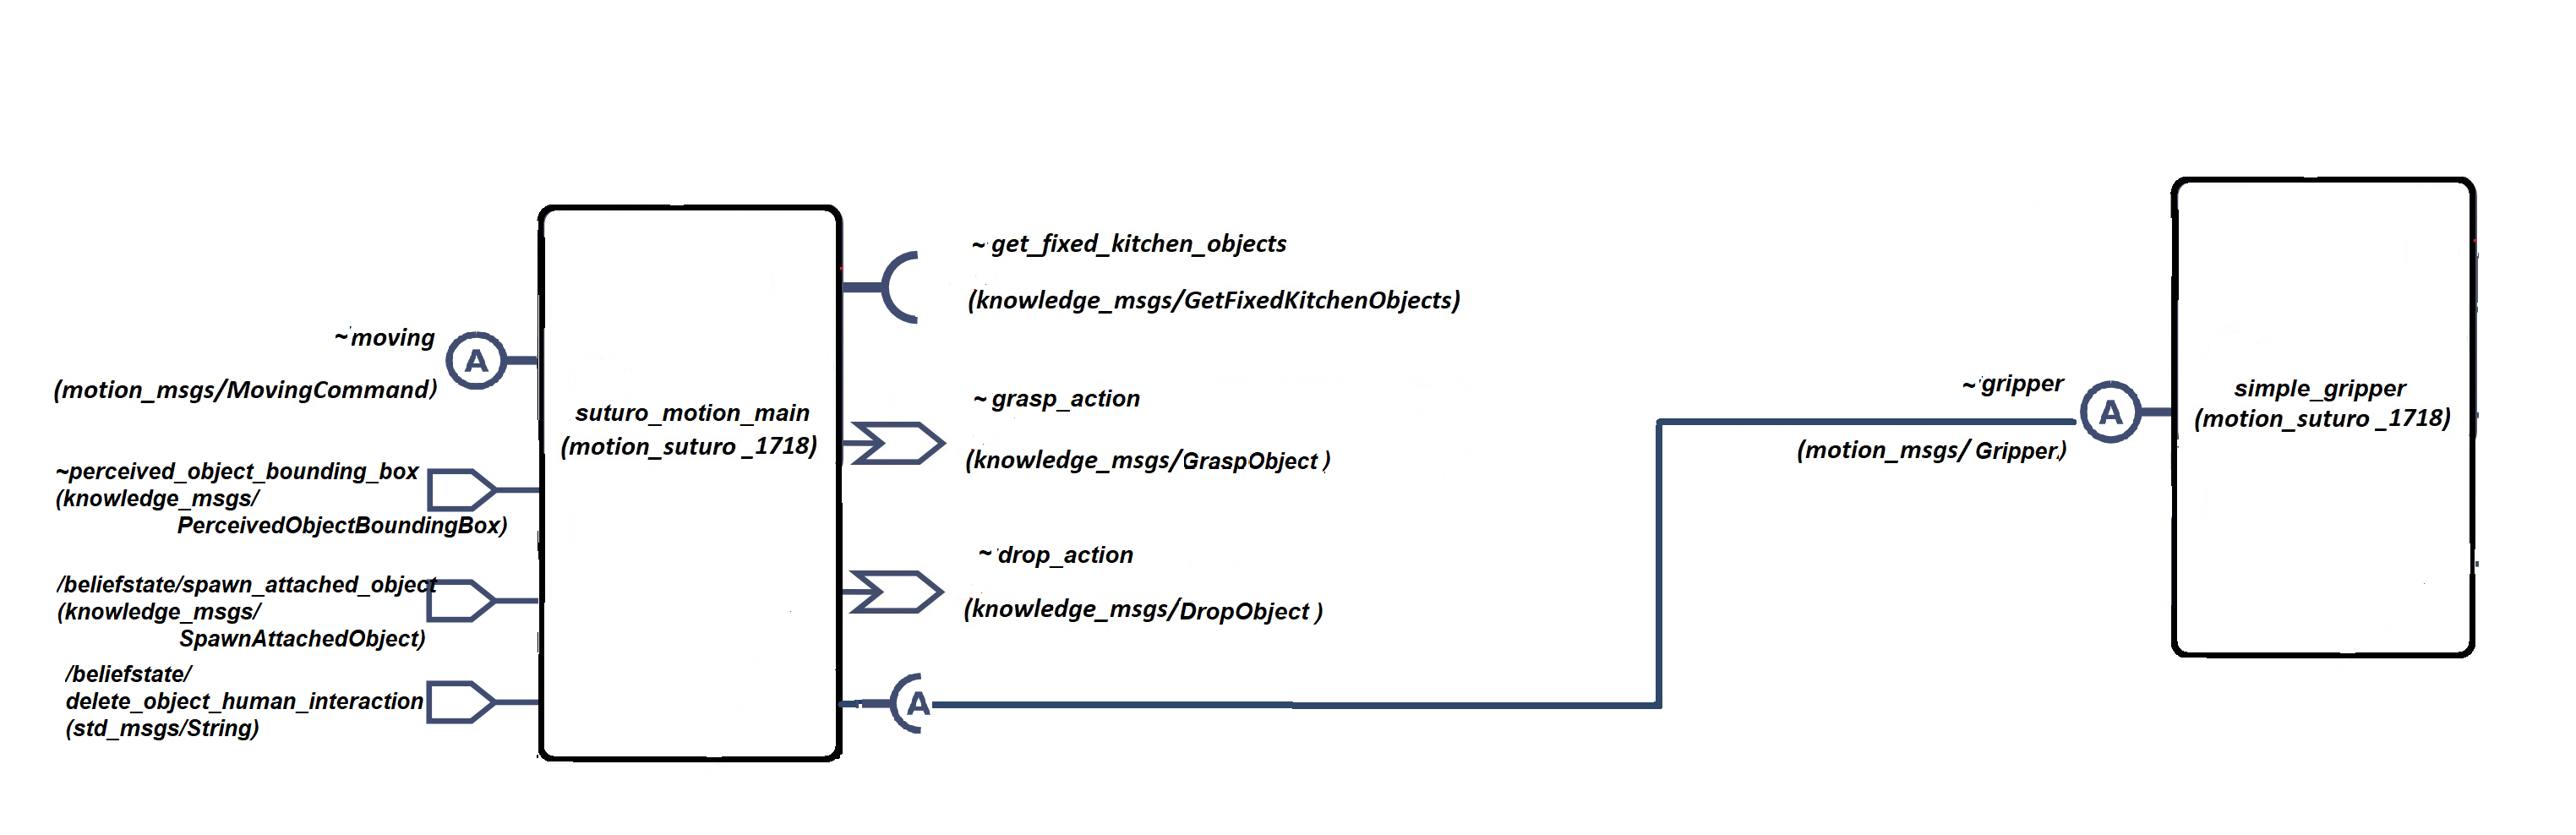
\includegraphics[width=\textwidth]
        {img/Architekturbild.png}
        \caption{\label{fig:motion_node} Architektur des Teilsystems der Gruppe 'Motion'}}
\end{figure}

Der Knoten '\textit{suturo\_motion\_main}' ist für das Verarbeiten eingehender Kommandos zum Bewegen der Arme bzw. der Endeffektoren zuständig. Dabei gibt es Kommandos für das Fahren der Arme in vordefinierte Posen oder in eine übergebene Pose. Zusätzlich können komplexere Operationen, wie das Schieben, Greifen oder Abstellen eines bestimmten Objektes ausgeführt werden.\\
Der Knoten '\textit{simple\_gripper}' wird dabei benutzt, um das Öffnen und Schließen des Endeffektors zu realisieren. Dieser Knoten wird von dem Hauptknoten '\textit{suturo\_motion\_main}' über einen Actionserver aufgerufen.\\

Im Folgenden werden die \textit{Schnittstellen}, der \textit{Ablauf} des Teilsystems und besonders \textit{hervorzuhebende} \textit{Algorithmen} beschrieben.\\

\newpage

\subsection{Schnittstellen - 'suturo\_motion\_main'}
\subsubsection{Angebotene Actions}
\textbf{MovingCommand}
\chapterauthor{Maximilian Bertram}
Vom Typ '\textit{motion\_msgs/MovingCommand}': \\

\subsubsection*{Definition des MovingCommands}
\begin{verbatim}
# goal definition
# goal_pose is used when an action, which is not the grasp action is called
# else goal_poses is used
geometry_msgs/PoseStamped goal_pose
geometry_msgs/PoseArray goal_poses

uint8 command
#Constants for command value
uint8 UNKNOWN=0
uint8 MOVE_DRIVE_POSE=1
uint8 MOVE_RIGHT_ARM=2
uint8 MOVE_LEFT_ARM=3
uint8 POKE_RIGHT_ARM=4
uint8 POKE_LEFT_ARM=5
uint8 GRASP_RIGHT_ARM=6
uint8 GRASP_LEFT_ARM=7
uint8 PLACE_RIGHT_ARM=8
uint8 PLACE_LEFT_ARM=9
uint8 MOVE_CARRY_POSE=10
uint8 MOVE_CARRY_POSE_RIGHT=11
uint8 MOVE_CARRY_POSE_LEFT=12

#The force when closing the gripper in newton default is set below
float64 force
float64 FORCE_DEFAULT=35

# Label of object which shell be grasped, placed or poked.
# Required because when an object gets grasped by robot,
# a message gets published from subgroup 'motion', which object
# has been grasped with which gripper (left or right).
# When the object gets placed somewhere, another message is published.
# These messages get published for knowledge's beliefstate, so that
# the knowledge component knows when an object get's grasped/placed somewhere.
# Additionaly required for some planningscene operations when grasping, 
# placing or poking an object.
string grasped_object_label

---
#result definition
bool successful
uint8 status
#Constants for status value
uint8 SUCCESS=0
uint8 OUT_OF_RANGE=1
uint8 COLLISION=2
uint8 UNMANAGEBLE_ERROR=3

---
#feedback definition
#bool finished
\end{verbatim}

Mit Hilfe der MovingCommandAction lassen sich alle von uns zur Verfügung gestellten Funktionen aufrufen. Es wurden Konstanten definiert, die die jeweilige Aktion beschreiben und in der Message-Definition vorhanden sind.

\subsubsection{Aufgerufene Actions}
\chapterauthor{Maximilian Bertram}
\textbf{Gripper}\\
Vom Typ '\textit{motion\_msgs/Gripper}': \\ \\
Wird eine Greif- oder Abstellaktion ausgeführt, wird über eine Nachricht an den Actionserver des Knotens '\textit{simple\_gripper}' der Gripper entsprechend geöffnet oder geschlossen.\\(Siehe Kapitel \ref{interfaceSimpleGripper} für Beschreibung des Actionservers.)\\


\subsubsection{Aufgerufene Services}
\chapterauthor{RH, MB}
\textbf{GetFixedKitchenObjects}\\
Vom Typ '\textit{knowledge\_msgs/GetFixedKitchenObjects}': \\ 
\begin{verbatim}
#This servicedefinition is for transferring the shape of the objects in
#the iai_kitchen.
#The Motion-component calls this service for getting the shape of the 
#kitchen-objects for its planningscene.
#The Knowledge-component reads these shapes out of an owl-file and 
#returns the data described below.

---

#The names of the kitchen objects
string[] names
#The path to the meshes of the kitchen objects
string[] meshes
#The names of the tf-frames of the kitchen objects. The kitchen object 
#meshes get spawned
#at the position of the corresponding frames.
string[] frames
\end{verbatim}

\subsubsection{Veröffentlichte Topics}
\textbf{GraspAction und DropAction}
\chapterauthor{Maximilian Bertram}

Wird ein Objekt erfolgreich abgestellt oder gegriffen, werden für den \textit{Beliefstate} von \textit{Knowledge} noch die entsprechenden \textit{Messages} gepublished: \\

\subsubsection*{Definition der GraspObject.msg}
\begin{verbatim}
#A message which gets published by Motion-component after grasping an object.

#The label of the grasped object.
string object_label

#The gripper used. See 'Gripper.msg' for more details.
Gripper gripper
\end{verbatim}

\subsubsection*{Definition der DropObject.msg}
\begin{verbatim}
#A message which gets published by Motion-component after dropping an object.

#The gripper used. See 'Gripper.msg' for more details.
Gripper gripper
\end{verbatim}

\subsubsection*{Definition der Gripper.msg}
\begin{verbatim}
#A message for defining constants for differencing between left and right gripper.

uint8 gripper
#constants for gripper
uint8 LEFT_GRIPPER = 1
uint8 RIGHT_GRIPPER = 2
\end{verbatim}

\newpage

\subsubsection{Benutzte Topics}
\textbf{PerceivedObjectBoundingBox}
\chapterauthor{Roman Haak}

Wird ein Objekt wahrgenommen, werden Daten über das Objekt auf dem Topic veröffentlicht. Diese werden genutzt, um das wahrgenommene Objekt zu unserer Planningscene hinzuzufügen.\\ Dabei sind folgende Daten über das Objekt in der Nachricht enthalten: \\

\subsubsection*{Definition der PerceivedObjectBoundingBox.msg}
\begin{verbatim}
#A message which gets published by knowledge when an object is perceived.

#The name of the object.
string object_label
#The path to the mesh of the object.
string mesh_path
#The pose the perceived object has.
geometry_msgs/PoseStamped pose
\end{verbatim}


\textbf{SpawnAttachedObject}
\chapterauthor{Roman Haak}

Kann ein Objekt nicht durch den Roboter gegriffen werden, wird der Mensch um Hilfe gefragt. Hat der Mensch dem Roboter das Objekt in den Gripper gegeben und wurde der Gripper geschlossen, werden Daten über den Vorgang über dieses Topic veröffentlicht. Diese werden genutzt, um das 'gegriffene' Objekt zu unserer Planningscene hinzuzufügen und an den entsprechenden Gripper des Roboters anzuheften.\\ Dabei sind folgende Daten über den Vorgang in der Nachricht enthalten: \\

\subsubsection*{Definition der SpawnAttachedObject.msg}
\begin{verbatim}
#A message which gets published by knowledge when an object is put
#in the gripper of the robot by a human.
#In which gripper the object was put can be determined by looking 
#in the header's frame id. The pose is given in the corresponding
#grippers tip frame.

#The pose of the object. 
geometry_msgs/PoseStamped pose
#The name of the object.
string object_label
\end{verbatim}



\textbf{DeleteObjectHumanInteraction}
\chapterauthor{Roman Haak}

Kann ein Objekt nicht durch den Roboter abgestellt werden, wird der Mensch um Hilfe gefragt. Hat der Mensch dem Roboter das Objekt aus dem Gripper genommen, werden Daten über den Vorgang über dieses Topic veröffentlicht. Diese werden genutzt, um das 'abgestellte' Objekt aus unserer Planningscene zu entfernen, weil es für die Bewegungsplanung ab diesem Zeitpunkt nicht mehr relevant ist.\\ Dabei besteht die Nachricht lediglich aus einem String, der den Namen des entfernten Objektes enthält.




\subsection{Schnittstellen - 'simple\_gripper'}
\chapterauthor{Maximilian Bertram}
\subsubsection{Angebotene Actions}
Vom Typ '\textit{motion\_msgs/Gripper}': \\
\subsubsection*{Definition der GripperAction}
\label{interfaceSimpleGripper}
\begin{verbatim}
#goal definition
#position of the space between the grippers in meters
float64 position
#force in newton (default =  20)
float64 effort
#which grpper to open/closed
uint8 gripper
#Constants for the gripper value
uint8 LEFT_GRIPPER=1
uint8 RIGHT_GRIPPER=2
---
#result definition
bool successful
---
#feedback definition
#bool finished
\end{verbatim}
\subsubsection{Aufgerufene Actions}
Die GripperAction-Message wird entsprechend geparsed und eine \\
 \textit{pr2\_ controllers\_ msgs::Pr2GripperCommandAction} erzeugt und gepublished. \\

\newpage

\subsection{Ablauf}
\chapterauthor{Maximilian Bertram, Roman Haak}
Der generelle Ablauf unseres Programms ist im Folgenden Ablaufdiagramm dargestellt.\\\\


\begin{figure}[!htb]
        \center{\includegraphics[scale=0.5]
        {img/Ablaufdiagramm.png}
        \caption{\label{fig:motion_node_flow_chart} Ablaufdiagramm 'Motion'}}
\end{figure}


\newpage

\subsection{Besonderheiten/Besondere Algorithmen}
In diesem Abschnitt werden erwähnenswerte Algorithmen beschrieben.\\
Dabei werden nacheinander mit Hilfe von Ablaufdiagrammen das Greifen, das Abstellen und das Schieben eines Objektes dargestellt.\\

\subsubsection{Algorithmus für das Greifen eines Objektes}
\chapterauthor{Roman Haak}

\begin{figure}[!htb]
        \center{\includegraphics[scale=0.3]
        {img/grasping_flowchart.png}
        \caption{\label{fig:motion_node_flow_chart_grasp} Ablaufdiagramm Greifen eines Objektes}}
\end{figure}

\newpage

\subsubsection{Algorithmus für das Abstellen eines Objektes}
\chapterauthor{Roman Haak}

\begin{figure}[!htb]
        \center{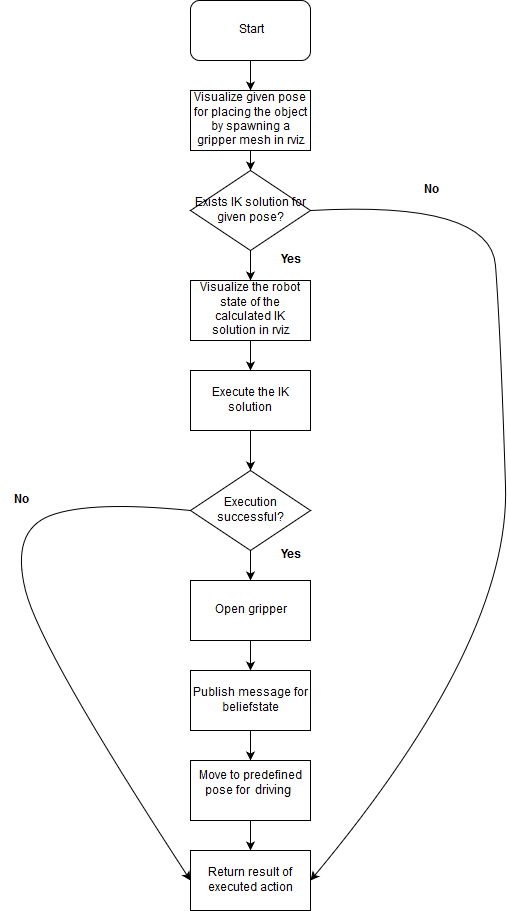
\includegraphics[scale=0.5]
        {img/placing_flowchart.png}
        \caption{\label{fig:motion_node_flow_chart_place} Ablaufdiagramm Abstellen eines Objektes}}
\end{figure}

\newpage

\subsubsection{Algorithmus für das Schieben eines Objektes}
\chapterauthor{Roman Haak}

\begin{figure}[!htb]
        \center{\includegraphics[scale=0.5]
        {img/poking_flowchart.png}
        \caption{\label{fig:motion_node_flow_chart_poke} Ablaufdiagramm Schieben eines Objektes}}
\end{figure}

\newpage

\subsection{Tests \& Evaluation}
\chapterauthor{Maximilian Bertram}

\subsubsection{Unit-Tests}
Um einen reibungslosen Entwicklungsprozess zu gewährleisten, war es nötig, unsere Lib-Funktionalität durch Unit-Tests abzudecken. Dies stellte uns vor diverse Herausforderungen. Zum einen lässt sich ROS-Funktionalität nicht testen; dadurch ist es nötig, die Core-Funktionalität unserer Library von ROS Funktionen zu befreien. Ein erster Ansatz war es, hierfür die \textit{ROSConnector-Klasse} anzulegen, welche einen Wrapper um ROS Funktionen darstellt und lediglich Methoden anbietet, die den Aufruf weiter an ROS delegiert. Dies sollte es ermöglichen, die nötigen ROS Aufrufe in unserer Library mit einem Mocking-Framework (in unserem Fall gMock) zu mocken und so Unit-Tests fahren zu können. Diesen Ansatz haben wir verfolgt, um dann leider festzustellen, dass gMock noch nicht von \textit{catkin} unterstützt wird. gMock ist nur in einer \textit{forked catkin version} verfügbar und es ist wohl geplant, das Framework in einer neueren Version von \textit{catkin} in das Main-Release zu integrieren. Daher haben wir uns dazu entschlossen, unsere Library soweit vorzubereiten, damit die \textit{Unit-Tests} nach dem Release und der Migration auf die neueste Version keinen großen Aufwand darstellen. Leider mussten wir feststellen, dass \textit{catkin build} beim Buildprozess keine Tests ausführt, sondern diese nur über \textit{catkin\_ make run\_ tests} ausgeführt werden können. Damit die Tests dennoch regelmäßig laufen und die Funktionalität der Lib regelmäßig getestet wird, wurde \textit{Continuous Integration} eingerichtet. Über den Dienst \textit{coverage.io} lässt sich zusätzlich ein \textit{Coveragereport} für die getesteten Packages erstellen, dadurch ist es möglich, Qualitätsstandards zu definieren und \textit{Mergerequests} nur bei ausreichender Testabdeckung zu akzeptieren. Leider war es uns nicht möglich, dies hier umzusetzen, da die OpenSource Registrierung von coverage.io zum Zeitpunkt der Umsetzung nicht funktionierte. \\
Der Sinn der Unit-Tests war es, die Zeit, bis Fehler bei der Entwicklung entdeckt werden, deutlich zu verkürzen und die Stelle der Fehler besser und schneller zu identifizieren. Dadurch wollten wir vor Allem die extrem langen Testzyklen auf dem echten Roboter verkürzen, um mehr Zeit für neue Features in der Entwicklung zu haben. \\

 $~$ \\
Damit sich Methoden mit gMock für die Tests leicht mocken lassen, sieht gMock eine \textit{virtual} Definition von Methoden, die gemockt werden sollen vor. Damit ergibt sich folgender Pseudocode für die \textit{ROSConnector-Klasse}: \\

\begin{verbatim}
class ROSConnector {
private:
    ROSClassInstance ros;
public:
    virtual returnType ROSMETHODNAME(Arg1 arg, Arg2 arg2, ...) {
        return ros.ROSMETHODNAME(arg, arg2, ...);
    }
}
\end{verbatim}

In der eigentlichen Library werden dann alle Funktionsaufrufe an ROS durch Funktionen der \textit{ROSConnector-Klasse} ersetzt. Für die \textit{Unit-Tests} werden diese Methoden dann mit gMock gemockt, um deren Rückgabewert im Testumfeld genau spezifizieren zu können und den Aufruf der \textit{ROSConnector-Klasse} zu verifizieren.



\subsubsection{Continuous Integration}
Um den Entwicklungsprozess weiter zu verbessern haben wir uns dazu entschieden, \textit{Continuous Integration} zu verwenden, um eine reibungslose Integration der Feature-Branches in den master-Branch zu gewährleisten. Dabei haben wir uns dazu entschieden, den CI-Dienst von \textit{Travis} zu nutzen. Einer der Hauptgründe hierfür ist die verhältnismäßig leichte Konfiguration über die \textit{.travis.yml}. Dabei musste \textit{catkin\_ make} verwendet werden, da \textit{catkin build} generell keine Tests ausführt. Dadurch war die Konfiguration von travis leider nicht trivial, da wir sogenannte \textit{private dependencies} in unserem Code verwenden; dies bezieht sich in unserem Fall auf die anderen \textit{SUTURO Pakete}. Diese mussten zuerst gecloned und gebaut werden, um im lokalen Buildrepository zur Verfügung zu stehen. Am besten lässt sich dies durch folgende kommentierte \textit{.travis.yml} zeigen. Relevant sind hier vor Allem die Bereiche \textit{install}, \textit{before\_ script} und \textit{script}: \\

\textit{install section of .travis.yml}
\begin{verbatim}
# Create a catkin workspace with the package under integration.
install:
  - mkdir -p ~/catkin_ws/src
  - cd ~/catkin_ws/src
  - catkin_init_workspace
  # Create the devel/setup.bash (run catkin_make with an empty workspace) and
  # source it to set the path variables.
  - cd ~/catkin_ws
  - catkin_make
  - source ~/catkin_ws/devel/setup.bash
  - cd ~/catkin_ws/src
  # Clone the private dependencies repositories
  - git clone https://github.com/menanuni/common_suturo1718.git
  - git clone https://github.com/menanuni/msgs_suturo_1718.git
  - cd ~/catkin_ws 
  # Install rosdeps from private deps
  - rosdep install -y --from-paths src --ignore-src --rosdistro $ROS_DISTRO -r
  # Add the package under integration to the workspace using a symlink.
  - cd ~/catkin_ws/src
  - ln -s $CI_SOURCE_PATH .
  - cd ~/catkin_ws
  # Build the private dependencies
  - catkin_make --pkg knowledge_msgs
  - catkin_make --pkg motion_msgs
  # Source the private dependencies
  - source ~/catkin_ws/devel/setup.bash
\end{verbatim}

\textit{before\_ script section of .travis.yml}

\begin{verbatim}
before_script:
  # source dependencies: install using wstool.
  - cd ~/catkin_ws/src
  - wstool init
  - if [[ -f $ROSINSTALL_FILE ]] ; then wstool merge $ROSINSTALL_FILE ; fi
  - wstool up
  # package depdencies: install using rosdep.
  - cd ~/catkin_ws
  - rosdep install -y --from-paths src --ignore-src --rosdistro $ROS_DISTRO -r

\end{verbatim}

\textit{script section of .travis.yml}

\begin{verbatim}
script:
  - source /opt/ros/$ROS_DISTRO/setup.bash
  - cd ~/catkin_ws
  # ensuring the path is set correctly.
  - source devel/setup.bash
  # Run the tests of package motion and motion gripper
  - catkin_make run_tests_motion
  - catkin_make run_tests_motion_gripper
\end{verbatim}

\newpage

\section*{Methodendokumentation Gruppe Vision}

\section{Vision}

\subsection{Überblick Vision}
\chapterauthor{Alexander Link}
Das Vision-Paket \footnote{im weiteren Verlauf auch Vision-Package, vision-node oder einfach Paket oder vision genannt} dient zur Akquirierung und Verarbeitung visueller Informationen durch die Kinect-Kamera des PR2-Roboters, sowie zur Verwendung dieser zum Klassifizieren gesehener Objekte und Bestimmen derer Posen.

\begin{figure}[!htb]
        \center{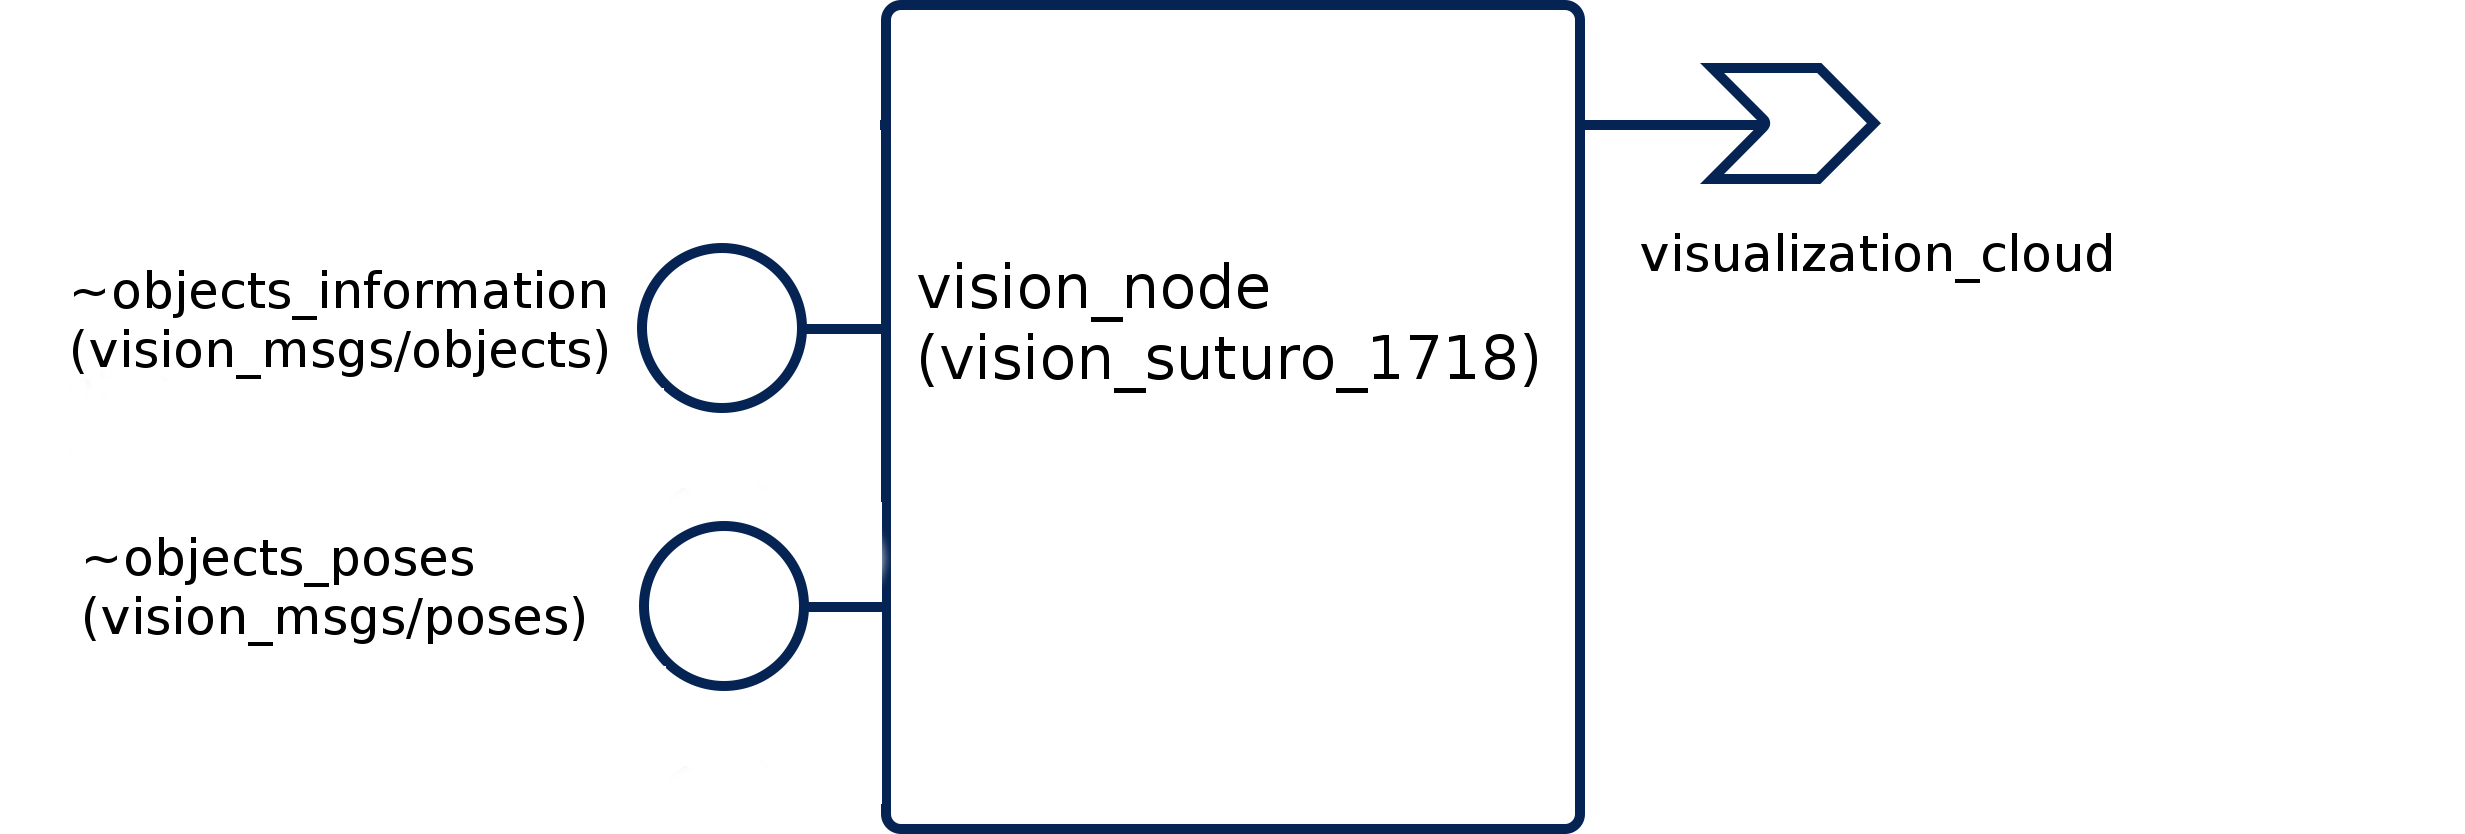
\includegraphics[width=\textwidth]
        {figures/vision_diagram_milestone_2.png}
        \caption{\label{fig:vision_node} Architektur der vision-node}}
\end{figure}
      
\subsection{Beschreibung des Teilsystems}
\chapterauthor{Tammo Wübbena, Update: Alexander Link}

\subsubsection{Abkürzungen durch short\_types.h}
\chapterauthor{Alexander Link (Doku), Beide (Code)}
Für bessere Lesbarkeit haben wir typedef Kürzel verwendet:
\begin{verbatim}
typedef pcl::PointCloud<pcl::PointXYZ>::Ptr PointCloudXYZPtr;
typedef pcl::PointCloud<pcl::PointXYZRGB>::Ptr PointCloudRGBPtr;
typedef pcl::PointCloud<pcl::Normal>::Ptr PointCloudNormalPtr;
typedef pcl::PointCloud<pcl::PointNormal>::Ptr PointCloudPointNormalPtr;
typedef pcl::PointCloud<pcl::PointXYZ> PointCloudXYZ;
typedef pcl::PointCloud<pcl::PointXYZRGB> PointCloudRGB;
typedef pcl::PointCloud<pcl::Normal> PointCloudNormal;
typedef pcl::PointIndices::Ptr PointIndices;
typedef std::vector<pcl::PointIndices> PointIndicesVector;
typedef std::vector<pcl::PointIndices::Ptr> PointIndicesVectorPtr;

typedef geometry_msgs::PointStamped PointStamped;
typedef pcl::PointCloud<pcl::VFHSignature308>::Ptr PointCloudVFHS308Ptr;
typedef sensor_msgs::PointCloud2 SMSGSPointCloud2;
typedef std::vector<pcl::PointCloud<pcl::PointXYZ>::Ptr> PointCloudXYZPtrVector;
\end{verbatim}

\subsubsection*{Perception}

\subsubsection{preprocessCloud}
\chapterauthor{Alexander Link (Doku), Tammo Wübbena (Code)}
\begin{verbatim}
findCluster(const PointCloudXYZPtr kinect)
Beschreibung: Wendet unsere Filter auf eine Punktwolke an.
@param: kinect Punktwolke
@return: Vorprozessierte Punktwolke
\end{verbatim}\label{func:preprocesscloud}

\subsubsection{segmentPlanes}
\chapterauthor{Alexander Link (Doku), Beide (Code)}
\begin{verbatim}
void segmentPlanes(PointCloudRGBPtr cloud_cluster)
Beschreibung: Segmentiert Flächen, die nicht für die gesuchten Objekte
relevant sind.
@param: PointCloud, aus der Flächen entfernt werden sollen.
\end{verbatim}\label{func:segmentplanes}

\subsubsection{findCluster}
\chapterauthor{Alexander Link (Doku), Beide (Code)}
\begin{verbatim}
std::vector<PointCloudRGBPtr> findCluster(PointCloudRGBPtr kinect)
Beschreibung: Findet die Objekte und gibt eine Punktwolke pro Objekt zurück.
@param: Punktwolke der Kinect
@return: Punktwolken der Objekte
\end{verbatim}\label{func:findcluster}

\subsubsection{findCenterGazebo}
\chapterauthor{Alexander Link (Doku), Beide (Code)}
\begin{verbatim}
geometry_msgs::PointStamped findCenterGazebo()
Beschreibung: Gibt einen künstlichen Punkt zurück (Den Mittelpunkt des
Modells, 
das an Gazebo übergeben wurde).
@return: Künstlicher 3D-Mittelpunkt
\end{verbatim}\label{func:findcentergazebo}


\subsubsection{findPoses}
\chapterauthor{Beide (Doku), Beide (Code)}
\begin{verbatim}
std::vector<geometry_msgs::PoseStamped> 
findPoses(const std::vector<PointCloudRGBPtr> clouds_in)
Beschreibung: Errechnet Position und Orientierung (Quaternion) der Objekte in den
übergebenen Punktwolken.
@param: Punktwolken der Objekte
@return: Posen der Objekte
\end{verbatim}\label{func:findposes}

\subsubsection{estimateSurfaceNormals}
\chapterauthor{Alexander Link (Doku), Beide (Code)}
\begin{verbatim}
PointCloudNormalPtr estimateSurfaceNormals(PointCloudRGBPtr input)
Beschreibung: Schätzt die Normalen einer Punktwolke.
@param: Punktwolke, zu der die Normalen berechnet werden sollen
@return: Normalen der übergebenen Punktwolke
\end{verbatim}\label{func:estimatesurfacenormals}

\subsubsection{apply3DFilter}
\chapterauthor{Alexander Link (Doku), Beide (Code)}
\begin{verbatim}
PointCloudRGBPtr apply3DFilter(PointCloudRGBPtr input, float x, float y, 
float z)
Beschreibung: Filtert eine Punktwolke, indem sie nur die Punkte in einem
bestimmten Bereich ((-x,x), (-y,y), (0.0,z)) erhält.
@param: Punktwolke, die gefiltert werden soll
		x,y,z Bereiche der Achsen für den Filter
@return Gefilterte Punktwolke
\end{verbatim}\label{func:apply3dfilter}

\subsubsection{estimatePlaneIndices}
\chapterauthor{Alexander Link (Doku), Beide (Code)}
\begin{verbatim}
PointIndices estimatePlaneIndices(PointCloudRGBPtr input)
Beschreibung: Errechnet die Indizes einer Fläche einer Punktwolke.
@param: Punktwolke, dessen Fläche ermittelt werden soll
@return Indizes der Fläche, wenn eine gefunden wurde
\end{verbatim}\label{func:estimateplaneindices}

\subsubsection{extractCluster}
\chapterauthor{Alexander Link (Doku), Beide (Code)}
\begin{verbatim}
PointCloudRGBPtr extractCluster(PointCloudRGBPtr input, PointIndices indices, 
bool negative);
Beschreibung: Extrahiert Objekt-Cluster anhand übergebener Punktwolke und
Indizes.
@param: input Punktwolke, aus der ein Cluster extrahiert werden soll
		indices Indizes der Punkte in input, die extrahiert werden sollen
		negative Entscheidet, ob Indizes extrahiert werden sollen (false) oder
		alle Punkte, außer den in Indizes angegebenen (true).
@return Objekt-Cluster Punktwolke
\end{verbatim}\label{func:extractcluster}

\subsubsection{mlsFilter}
\chapterauthor{Alexander Link (Doku), Beide (Code)}
\begin{verbatim}
PointCloudRGBPtr mlsFilter(PointCloudXYZPtr input);
Beschreibung: Glättet Punktwolke unter Verwendung eines Moving-Least-Squares
Algorithmus.
@param: Punktwolke, die mittels MLS-Algorithmus geglättet wird
@return Geglättete Punktwolke
\end{verbatim}\label{func:mlsfilter}

\subsubsection{voxelGridFilter}
\chapterauthor{Alexander Link (Doku), Beide (Code)}
\begin{verbatim}
PointCloudRGBPtr voxelGridFilter(PointCloudRGBPtr input)
Beschreibung: Filtert eine Punktwolke mit dem Voxel-Gitter-Filter.
@param: Zu filternde Punktwolke
@return Mit einem Voxel-Gitter gefilterterte (und damit gedownsamplete)
Punktwolke
\end{verbatim}\label{func:voxelgridfilter}

\subsubsection{outlierRemoval}
\chapterauthor{Alexander Link (Doku), Beide (Code)}
\begin{verbatim}
PointCloudRGBPtr outlierRemoval(PointCloudRGBPtr input)
Beschreibung: Entfernt Punkte aus Punktwolke, die als zu weit außen liegend
(outlier) oder als Rauschen erkannt werden.
@param: Punktwolke, die von Rauschen befreit werden soll
@return Gefilterte Punktwolke
\end{verbatim}\label{func:outlierremoval}

\subsubsection{cvfhRecognition}
\chapterauthor{Alexander Link (Doku + Code)}
\begin{verbatim}
PointCloudVFHS308Ptr cvfhRecognition(PointCloudRGBPtr input)
Beschreibung: Errechnet features eines Objekts in einer Punktwolke als
VFHSignature308
@param: Punktwolke, dessen features berechnet werden sollen
@return Features als VFHSignature308
\end{verbatim}\label{func:cvfhRecognition}

\subsubsection{euclideanClusterExtraction}
\chapterauthor{Alexander Link (Doku + Code)}
\begin{verbatim}
std::vector<PointCloudRGBPtr> euclideanClusterExtraction(PointCloudRGBPtr
input)
Beschreibung: Trennt cluster einer Punktwolke voneinander.
@param: Punktwolke
@return Eine Punktwolke pro cluster/Objekt
\end{verbatim}\label{func:euclideanClusterExtraction}

\subsubsection{iterativeClosestPoint}
\chapterauthor{Alexander Link (Doku), Tammo Wübbena (Code)}
\begin{verbatim}
PointCloudRGBPtr iterativeClosestPoint(PointCloudRGBPtr input,
                                       PointCloudRGBPtr target)
Beschreibung: Errechnet Ausrichtung eines Objekts zu einem Ziel anhand eines
iterativen 
			  Closest-Point-Algorithmus.
@param: input Punktwolke, target Punktwolke
@return Punktwolke
\end{verbatim}\label{func:iterativeClosestPoint}

\subsubsection{produceColorHist}
\chapterauthor{Alexander Link (Doku), Tammo Wübbena (Code)}
\begin{verbatim}
std::vector<uint64_t> produceColorHist
(pcl::PointCloud<pcl::PointXYZRGB>::Ptr  cloud)
Beschreibung: Errechnet ein Farbhistogramm einer Punktwolke.
@param: input Punktwolke eines Objekts, dessen Farbhistogramm errechnet werden
soll
@return Farbhistogramm als floats (r,g,b)
\end{verbatim}\label{func:produceColorHist}

\subsubsection{getCVFHFeatures}
\chapterauthor{Alexander Link (Doku), Tammo Wübbena (Code)}
\begin{verbatim}
void getCVFHFeatures(std::vector<PointCloudRGBPtr> all_clusters,
std::vector<float> current_features_vector)
Beschreibung: Errechnet CVFH-features von Punktwolken
@param: Punktwolken der Objekte, deren CVFH-features errechnet werden sollen
@return: CVFH features (Histogramme der Winkel zwischen einer zentralen
viewpoint direction und jeder Normalen
\end{verbatim}\label{func:getcvfhfeatures}

\subsubsection{getColorFeatures}
\chapterauthor{Alexander Link (Doku), Tammo Wübbena (Code)}
\begin{verbatim}
void getColorFeatures(std::vector<PointCloudRGBPtr> all_clusters,
std::vector<uint64_t> color_features_vector)
Beschreibung: Errechnet Farbfeatures von Punktwolken
@param: Punktwolken der Objekte, deren Farbfeatures errechnet werden sollen
	    Vektor für Farbfeatures, der befüllt wird
\end{verbatim}\label{func:getcolorfeatures}

\subsubsection{getTargetByLabel}
\chapterauthor{Alexander Link (Doku), Tammo Wübbena (Code)}
\begin{verbatim}
PointCloudRGBPtr getTargetByLabel(std::string label)
Beschreibung: Lädt die PCD-Datei des Objekts, das zum übergebenen label
gehört.
@param: String label
@return Objekt-Punktwolke aus der jeweiligen PCD-Datei
\end{verbatim}\label{func:gettargetbylabel}


\subsection*{vision\_node}
\chapterauthor{Alexander Link (Doku), Beide (Code)}
\subsubsection{sub\_kinect\_callback}
\begin{verbatim}
void sub_kinect_callback(PointCloudRGBPtr kinect)
Beschreibung: Callback-Funktion für das kinect topic. Speichert die PointCloud
ab, sodass sie bereitsteht, wenn sie zur Prozessierung benötigt wird.
@param: Punktwolke des kinects
\end{verbatim}\label{func:subkinectcallback}
\subsubsection{start\_node}
\begin{verbatim}
void start_node(int argc, char **argv)
Beschreibung: Startet die Node zur Prozessierung von Punktwolken und der
Kommunikation mit anderen Nodes.
@param: argc und argv ungenutzt
\end{verbatim}\label{func:startnode}
\subsubsection{getObjects}
\begin{verbatim}
bool getObjects(	vision_suturo_msgs::objects::Request &req, 
			    vision_suturo_msgs::objects::Response &res)
Beschreibung: Service zum Extrahieren von Objekten und deren Informationen aus
einer Szene.
@param: req leere request, res Antwort mit den extrahierten Objekten nach
ObjectsInfo.msg
@return true wenn service call erfolgreich, ansonsten false
\end{verbatim}\label{func:getobjects}

\subsubsection{getPoses}
\begin{verbatim}
bool getObjects(vision_suturo_msgs::objects::Request &req, 
vision_suturo_msgs::objects::Response &res)
Beschreibung: Service zum ermitteln von Posen der zuvor extrahierten Objekte.
@param: req index und label des Clusters, für den eine Pose bestimmt werden soll; 
res Antwort mit Pose zum Objekt
ObjectsInfo.msg
@return true wenn service call erfolgreich, ansonsten false
\end{verbatim}\label{func:getposes}



\subsection*{CloudTransformer}
\chapterauthor{Alexander Link (Doku + Code)}

\subsubsection{extractAbovePlane}
\begin{verbatim}
PointCloudRGBPtr CloudTransformer::extractAbovePlane(PointCloudRGBPtr input)
Beschreibung: Findet die Hauptfläche (-> Tischplatte) und extrahiert nur die
Punkte über dieser Fläche.
@param: Punktwolke
@return Extrahierte Punktwolke (ohne die Hauptfläche)
\end{verbatim}\label{func:extractaboveplane}
\subsubsection{transform}
\begin{verbatim}
PointCloudRGBPtr CloudTransformer::transform(const PointCloudRGBPtr cloud,
std::string target_frame,
                 std::string source_frame)
Beschreibung: Transformiert eine Punktwolke in einen anderen frame.
@param: cloud Punktwolke, target_frame, source_frame
@return Transformierte Punktwolke
\end{verbatim}\label{func:transform}

\subsection*{classifier}
\chapterauthor {Alexander Link (Doku \& Code)}

\subsubsection{train}
\begin{verbatim}
bool classifier::train(std::string directory, bool update)
Beschreibung: Trainiert der Klassifizierer unter Verwendung von .csv-Dateien,
die sich in den Unterordnern des gegebenen Pfades befinden. Jeder Unterordner
sollte nach dem jeweiligen Label benannt sein.
@param directory: Der Pfad, der Unterordner mit .csv-Dateien enthält
@param update: True lässt den Klassifizierer neu trainieren. False führt dazu,
dass er Daten eines vorhergegangenen Trainings lädt.
@return True wenn erfolgreich, ansonsten false.
\end{verbatim}\label{func:train}

\subsubsection{classify}
\begin{verbatim}
std::string classifier::classify(std::vector<uint64_t> color_features,
std::vector<float> cvfh_features)
Beschreibung: Klassifiziert eine einzelne Punktwolke anhand ihrer Features.
classifier::train() muss zuerst erfolgreich aufgerufen worden sein.
@param color_features: Errechnet durch produceColorHist()
@param cvfh_features: Errechnet durch cvfhRecognition()
@return Das Label des klassifizierten Objekts. War die Klassifizierung
nicht erfolgreich, wird ein leerer String zurückgegeben.
\end{verbatim}\label{func:classify}

\subsubsection{has\_suffix}
\begin{verbatim}
bool classifier::has_suffix(std::string s, std::string suffix)
Beschreibung: Entscheidet, ob ein String einen suffix enthält.
@param s: String
@param suffix: String, der im String s enthalten sein soll
@return true, wenn s in suffix enthalten ist. Ansonsten false.
\end{verbatim}\label{func:hassuffix}

\subsubsection{read\_from\_file}
\begin{verbatim}
std::vector<float> classifier::read_from_file(std::string full_path, 
std::vector<float> parsedCsv)
Beschreibung: Extrahiert Features aus einer .csv-Datei
@param full_path: Pfad zur .csv-Datei
@param parsedCsv: Float-Vektor, an die die Features angehängt werden
@return parsedCsv + neue floats aus .csv-Datei
\end{verbatim}\label{func:readfromfile}


\subsection*{saving}
\chapterauthor{Alexander Link (Doku), Beide (Code)}
Hilfsfunktionen zum Speichern von Punktwolken als .PCD-Dateien.

\begin{verbatim}
void savePointCloudRGBNamed(pcl::PointCloud<pcl::PointXYZRGB>::Ptr cloud,
                            std::string filename);
                            
void savePointCloudXYZ(pcl::PointCloud<pcl::PointXYZ>::Ptr cloud);

void savePointCloudXYZNamed(pcl::PointCloud<pcl::PointXYZ>::Ptr cloud,
std::string filename);

void savePointCloudNormal(pcl::PointCloud<pcl::Normal>::Ptr cloud);

void savePointCloudPointNormal(pcl::PointCloud<pcl::PointNormal>::Ptr cloud);

void savePointCloud(pcl::PointCloud<pcl::PointXYZ>::Ptr objects,
                    pcl::PointCloud<pcl::PointXYZ>::Ptr kinect,
                    pcl::PointCloud<pcl::Normal>::Ptr normals);
\end{verbatim}


\subsection*{viewer}
\chapterauthor{Alexander Link (Doku), Tammo Wübbena (Code)}
Hilfsfunktionen zur Darstellung von Punktwolken.
Enthält auch den momentan ungenutzten Visualization Marker.

\begin{verbatim}
void visualizePointCloud(pcl::PointCloud<pcl::PointXYZ> cloud);

void visualizeNormals(pcl::PointCloud<pcl::PointXYZ>::Ptr cloud,
pcl::PointCloud<pcl::Normal>::ConstPtrnormals);

visualization_msgs::Marker publishVisualizationMarker
(geometry_msgs::PointStamped point);
\end{verbatim}


\subsection{Schnittstellen}
\chapterauthor{Tammo Wübbena}

\subsubsection{Service Server /vision\_suturo/objects\_information}
\begin{verbatim}
objects.srv
@request: -
@response: ObjectsInfo msg (
							normal_features (VHFSignature308 as array)
							color_features (Color Histogram as array)
							object_amount (Number of objects in scene)
							object_information (additional information)
							object_errors (errors while extracting)
							)
\end{verbatim}
Gibt Anzahl, Features von den in einer Szene erkannten Objekten (Clustern) zurück. Der Service kann weitere Informationen und bei Problemen unterschiedliche Fehlermeldungen zurückgeben.
\\ \\
Die \textit{normal\_features} vom Typ VFHSignature308 und \textit{color\_features} (acht bins) aller Objekte werden konkateniert in Arrays festgehalten. 
Da die Länge der Features für ein Objekt immer gleich ist, kann durch die Anzahl der erkannten Objekte die Länge insgesamt ermittelt werden.

\subsubsection{Service Server /vision\_suturo/objects\_poses}

\begin{figure}[!htb]
        \center{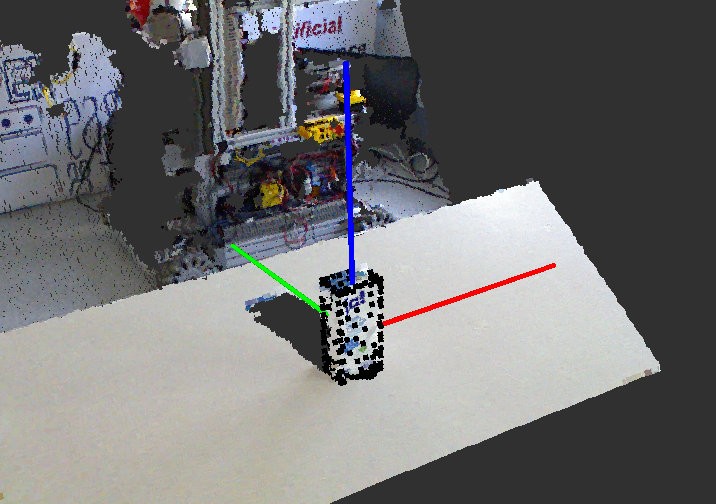
\includegraphics[width=0.6 \textwidth]
        {img/vision_pose_service.png}
        \caption{} Ausgabe der Ausrichtung für ein Objekt durch den Pose Service}
\end{figure}


\begin{verbatim}
poses.srv
@request: string, uint8 (label of classified (recognized) object and its number
in the array given by the ObjectsInfo.msg)
@response: ObjectsInfo msg (
							poses (the pose of the requested object)
							)
\end{verbatim}
Nachdem der Service objects\_information aufgerufen wurde, werden die dadurch erzeugten Features und klassifizierten Objekte mit einem Label versehen und an Planning weitergeleitet. Danach werden die Objekte von unserem Paket bearbeitet und die Pose durch Vergleich mit den jeweiligen Meshes ermittelt. Im Anschluss werden die Posen zurück an Planning übergeben.

\subsubsection{Subscriber REAL\_KINECT\_POINTS\_FRAME}
\begin{verbatim}
@response: PointCloudRGBPtr kinect
\end{verbatim}
Gibt eine Punktwolke unseres Sichtfelds (Szene oder Scene) zurück. Dabei wird auf das Topic \textit{/kinect\_head/depth\_registered/points} horcht. Alternativ kann mit \textit{SIM\_KINECT\_POINTS\_FRAME} auf \textit{/head\_mount\_kinect/depth\_registered/points} auf Simulationsdaten gehorcht werden.
\\ \\
Die Callback-Funktion wird im loop immer wieder aufgerufen, solange die Node noch aktiv ist bzw. der roscore-server besteht.

\subsection{Programmablauf}
\chapterauthor{Alexander Link \& Tammo Wübbena}
\subsubsection{Schritt 1: Vorbereitung}
Die Services, der Visualization-Publisher und der Kinect-Subscriber werden gestartet. Je nach Einstellung wird der Klassifizierer trainiert, oder lädt Daten vom Training aus vorhergegangenen Nodestarts.

\begin{figure}[!htb]
        \center{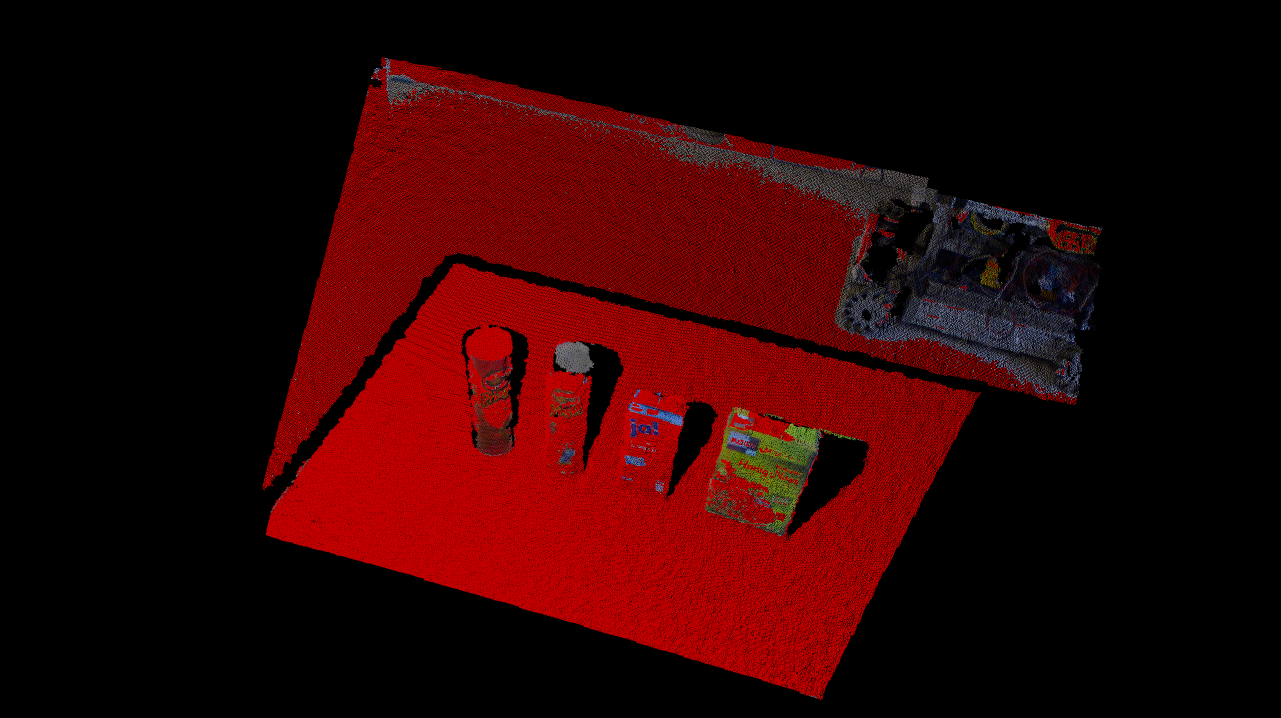
\includegraphics[width=0.6 \textwidth]
        {img/vision_1_all.png}
        \caption{} Ansicht einer beispielhaften Punktwolke, die wir durch den Kinect-Sensor zur Verfügung gestellt bekommen.}
\end{figure}

\subsubsection{Schritt 2: Serviceaufruf \textit{/vision\_suturo/objects\_information}}
Jedes mal, wenn der Service \textit{/vision\_suturo/objects\_information} durch Planning aufgerufen wird, wird die Funktion \textit{findCluster} in perception.h ausgeführt. 
\\
\subsubsection{Schritt 3: Filterung und Segmentierung} 
In \textit{findCluster} wird die Punktwolke zunächst folgendermaßen vorbearbeitet:

\begin{itemize} 
\item Ein PassThrough Filter, der den Sichtbereich begrenzt.
\item Ein VoxelGrid Filter zum Downsampling der eingehenden Punktwolke, indem für viele kleine 3-dimensionale Boxen der Mittelpunkte aller enthaltenden Punkte berechnet wird.
\item Ein MovingLeastSquares Filter, der Flächen begradigt, um Ungenauigkeiten der Daten vorzubeugen.
\item Entfernen aller Punkte, die nicht zum größten Cluster in der Szene gehören.
\item Finden der Grundfläche (für gewöhnlich die Tischplatte). Alle Punkte, die sich nicht oberhalb der Tischplatte befinden, werden entfernt. Anschließend wird die Grundfläche selbst entfernt.

\begin{figure}[!htb]
        \center{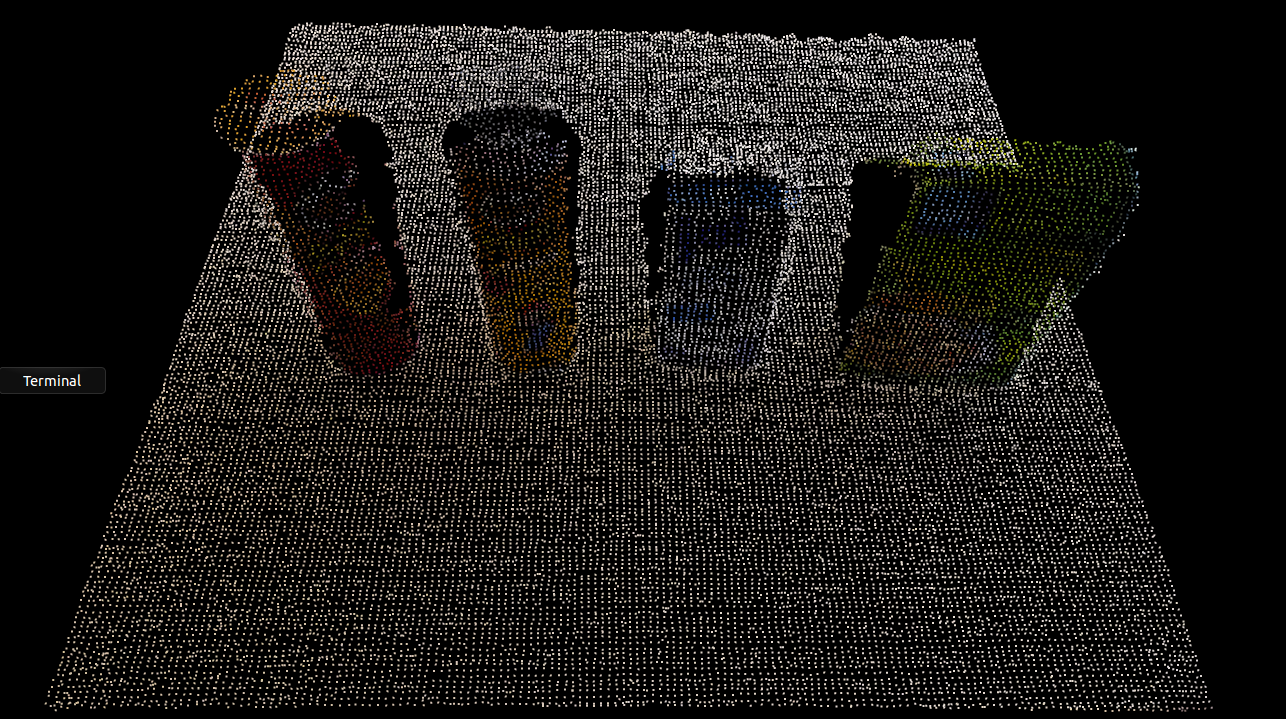
\includegraphics[width=0.6 \textwidth]
        {img/vision_2_preprocessed.png}
        \caption{} Ansicht der Zwischenergebnisse mitsamt Grundfläche}
\end{figure}

\item Entfernen von weiteren Flächen, die zu groß sind, um zum gesuchten Objekt gehören zu können. Dies passiert mehrmals, wenn es mehrere solcher Flächen im Sichtfeld gibt.
\end{itemize}

\subsubsection{Schritt 4: Cluster Extraktion}
Mit \textit{EuclideanClusterExtraction} werden die nun segmentierten Objekte (alle noch in einer Punktwolke zusammengefasst) extrahiert und in einzelne Cluster gespeichert.

\begin{figure}[!htb]
        \center{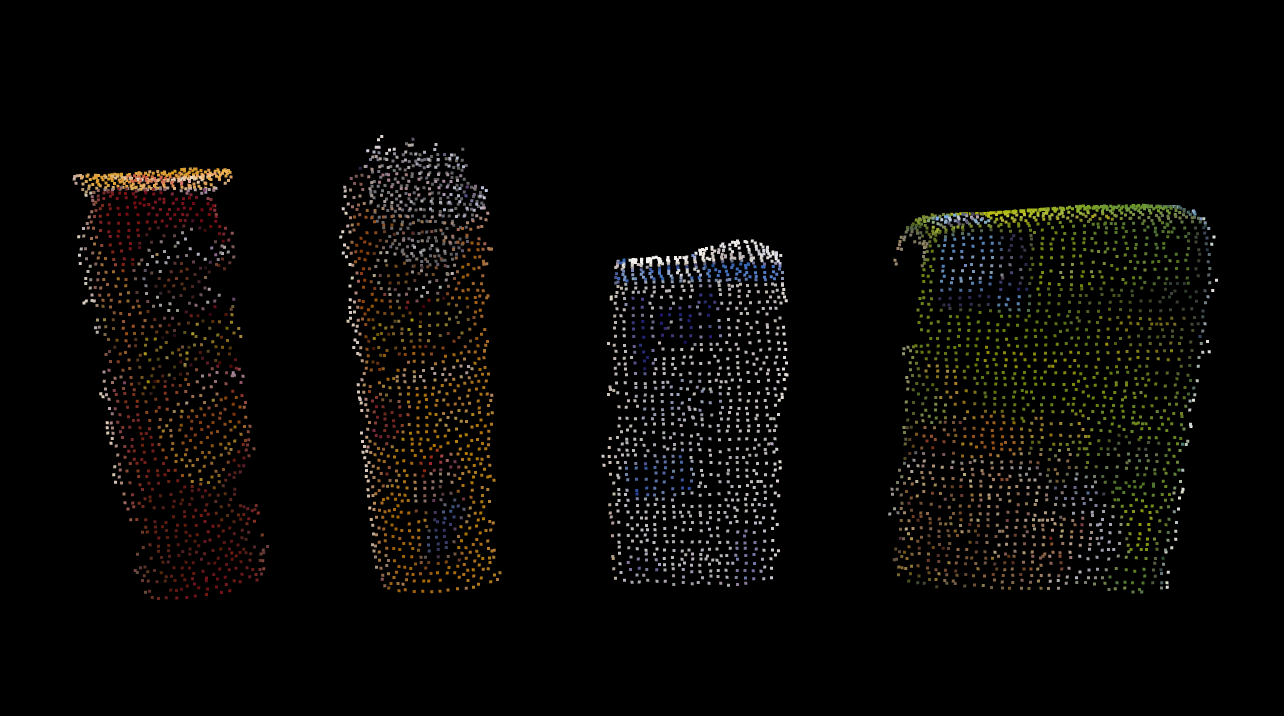
\includegraphics[width=0.6 \textwidth]
        {img/vision_3_withoutplane.png}
        \caption{} Ansicht der einzelnen extrahierten Cluster}
\end{figure}

\subsubsection{Schritt 5: Berechnen von Features und Klassifizierung}
Es werden CVFH- und Farbfeatures für die Klassifikation berechnet. Mithilfe des in Schritt 1 mit Daten befüllten Klassifizierers wird nun festgestellt, welche Gegenstände sich in der Szene befinden.
\\
\subsection{Schritt 6: Servicerückgabe}
Zurückgegeben werden die Labels der einzelnen erkannten Objekte sowie die Anzahl der Objekte, die sich in der Szene befinden.
\\
\subsection{Schritt 7: Serviceaufruf \textit{/vision\_suturo/objects\_poses}}
Wenn Planning jetzt den Service \textit{/vision\_suturo/objects\_poses} aufruft, wird übergeben, für welches der Objekte, die wir zuvor in \textit{/vision\_suturo/objects\_information} festgestellt haben, die Pose errechnet werden soll.

\subsubsection{Schritt 8: Angleichen von Mesh und Objekt (Cluster)}
Das Objekt wird mit ihrem jeweiligen Mesh abgeglichen und durch Iterative Closest Point Algorithmen werden die Rotationsmatrizen zu den Posen ermittelt.

\subsubsection{Schritt 9: Berechnen des Quaternions }
Die im vorherigen Schritt errechneten Rotationsmatrizen werden verwendet, um mit Hilfe eines Transforms das Quaternion zu berechnen, dass die Orientierung des Objekts darstellt. 

\subsubsection{Schritt 10: Berechnen des Mittelpunkts }
Der Mittelpunkt des angeglichenen Meshes (als Punktwolke) wird errechnet und als Vektor gespeichert.
\\
\subsubsection{Schritt 11: Befüllen der MSG }
Die Message wird mit dem Mittelpunkt als Vektor und der Orientierung als Quaternion befüllt und weiter an Planning gesendet.

\subsection*{Visualization-Publisher}
Der Visualization-Publisher gibt zu Debugging-Zwecken die extrahierten Cluster als einzelne Punktwolke aus.

\begin{figure}[!htb]
        \center{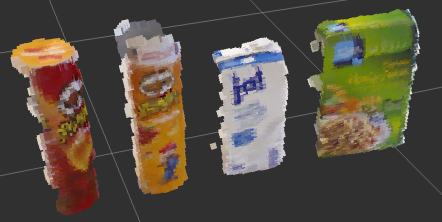
\includegraphics[width=0.6 \textwidth]
        {img/vision_visualization_object.png}
        \caption{} Debug-Ausgabe der erkannten Objekte durch einen PointCloud2-Publisher.}
\end{figure}

\newpage
\section{Nutzungsbeschreibung}

\subsection{Installation und Ausführung von Planning}

\subsubsection{Installation}
\chapterauthor{Vanessa Hassouna}
\begin{itemize}


\item[a] Sind alle Systeme lauffähig (Vision,Knowledge und Motion), muss für Planning folgendes Repository hinzufügt werden: \url{https://github.com/menanuni/planning_suturo_1718.git}. 

\item[b] Ist die Arbeitsumgebung vollständig gebaut, wird CRAM installiert \url{http://cram-system.org/installation}.

\item[c] Nun wird die Entwicklungsumgebung installiert mit: \textbf{sudo apt-get install emacs}. Achtung: Bei der Verwendung von Ubuntu 14.04 muss der neueste Lisp 'compiler' noch hinzugefügt werden \url{https://sourceforge.net/projects/sbcl/files/sbcl/1.3.1/
} (meistens x86-64 Version). Diese Datei entpacken und im Terminal (im richtigen Ordner) den Befehl: \textbf{sh install.sh} eingeben.
\end{itemize}

\subsubsection{Ausführung}
\chapterauthor{Vanessa Hassouna}
\begin{itemize}

\item Zuerst muss im Terminal \textbf{roslisp\_repl} eingegeben werden, daraufhin startet emacs. 

\item Nun wird in der Repl (dort wo cl-user steht) ein "\textbf{,}" (ausgesprochen Komma) eingegeben.

\item Nun wird \textbf{r-l-s} eingegeben und mit \textbf{ENTER} bestätigt. Es folgt die Eingabe des Namens für ein Paket: \textbf{planning\_main\_programm} wird mit zweimaligem Befehl \textbf{ENTER} bestätigt.

\item Zum Schluss wird noch in dem cl-user Fenster \textbf{(planning-main-programm::main)} eingegeben und mit \textbf{ENTER} bestätigt (die Klammern gehören auch dazu).
\end{itemize}


\subsection{Installation und Ausführung von Motion}

\subsubsection{Installationsanleitung}
\chapterauthor{Maximilian Bertram}

\begin{itemize}
\item[a] Zunächst müssen folgende Repositories in den source-Ordner des Workspaces hinzugefügt werden:  \\
\url{https://github.com/menanuni/motion_suturo_1718} \\
\url{https://github.com/menanuni/msgs_suturo_1718} \\
\url{https://github.com/menanuni/knowledge_suturo_1718} \\
\url{https://github.com/menanuni/vision_suturo_1718} \\
\url{https://github.com/menanuni/common_suturo1718} \\

\item[b] Es muss das MoveIt Framework installiert werden, dazu im Terminal: \\
\textit{sudo apt-get update} \\
\textit{sudo apt-get install ros-indigo-moveit} \\
\textit{echo  \grqq{}source /opt/ros/indigo/setup.bash\grqq{} \textgreater\textgreater \textasciitilde{ }/.bashrc} \\

\item[c] Jetzt kann das System über \textit{catkin build} gebaut werden.
\end{itemize}

Den Stand der für Stand  des 2. Meilensteins findet sich unter folgendem Tag: \\
\url{https://github.com/menanuni/motion_suturo_1718/releases/tag/milestone2} \\

\subsubsection{Starten der Nodes}
\chapterauthor{Roman Haak}
\begin{itemize}

\item Soll das System im Kontext des echten Roboters benutzt werden, startet man zunächst über \textit{roslaunch kitchen\_model\_export knowledge\_export\_service.launch} ein Teilsystem von \textit{Knowledge}.

\item Unser Teilsystem wird dann über \textit{roslaunch motion motion\_main\_start.launch} gestartet, falls es im Kontext einer Simulation ausgeführt werden soll, bzw. über \textit{roslaunch motion motion\_main\_start\_real\_pr2.launch}, falls das Ausführen des Systems auf dem echten PR2 gewünscht ist.

\item Dann können Befehle an den Actionserver unseres Knotens über das Topic \textit{/moving/goal} abgesetzt werden. Zur Erläuterung des Actionservers siehe Dokumentation der Gruppe \textit{motion}.
\end{itemize}

\subsection{Installation und Ausführung von Vision}

\subsubsection{Installation (mit gazebo)}
\chapterauthor{Alexander Link}

\textbf{Voraussetzungen}

\begin{itemize}
\item Ubuntu 14.04
\item ROS Indigo
\item Catkin tools
\item Gazebo 2.2.x
\item OpenCV 3.3.0
\end{itemize}

\textbf{.bashrc}

Folgendes muss zur .bashrc (oder zshrc) hinzugefügt werden:
\begin{itemize}
\item \textit{export KINECT1=true}
\item \textit{export GAZEBO\_MODEL\_PATH= \$HOME/catkin\_ws/vision\_suturo\_1718/vision/models}
\item \textit{export GAZEBO\_RESOURCE\_PATH= \$HOME/catkin\_ws/vision\_suturo\_1718/vision/worlds}
\end{itemize}

\textbf{Setup}

\begin{itemize}
\item Gazebo installieren: \textit{sudo apt-get install ros-indigo-pr2-simulator}

\item Sollten Probleme auftreten, könnte dies durch ein Update von gazebo auf v2.2.6 gelöst werden:
\\
\textit{sudo sh -c 'echo ''deb http://packages.osrfoundation.org/gazebo/ubuntu trusty main'' $>$ \\ 
/etc/apt/sources.list.d/gazebo-latest.list'}
\\
\textit{wget http://packages.osrfoundation.org/gazebo.key -O - | sudo apt-key add -}
\\
\textit{sudo apt-get update}


\item OpenCV 3.3.0 herunterladen und folgendermaßen installieren: \\

\textit{mkdir build} \\
\textit{cd build/} \\
\textit{cmake -D CMAKE\_BUILD\_TYPE=RELEASE -D \\ 
CMAKE\_INSTALL\_PREFIX=/usr/local -D FORCE\_VTK=ON -D \\ 
WITH\_TBB=ON -D WITH\_V4L=ON -D WITH\_QT=ON -D \\ 
WITH\_OPENGL=ON -D WITH\_CUBLAS=ON -D \\ 
CUDA\_NVCC\_FLAGS="-D\_FORCE\_INLINES" -D WITH\_GDAL=ON \\ 
-D WITH\_XINE=ON -D BUILD\_EXAMPLES=ON ..} \\
\textit{make -j $(($(nproc) + 1))} \\
\textit{sudo make install} \\



\item Folgende Pakete in den src-Ordner eines catkin workspaces klonen:\\
        \textbf{vision\_suturo\_1718} (this package) \\
        \textbf{msgs\_suturo\_1718}
\item Erst "\textit{catkin build object\_detection}" nutzen, um die messages zu bauen.
\item Dann "\textit{catkin build}" benutzen, um alles andere zu bauen.

\end{itemize}

\textbf{Kinect benutzen}
\begin{itemize}
\item \textit{sudo apt install ros-indigo-freenect-launch freenect libfreenect-bin}
\item \textit{roslaunch freenect\_launch freenect-registered-xyzrgb.launch}
\item (Optional) \textit{roslaunch vision vision\_kinect.launch}
\end{itemize}

\textbf{Dateien speichern}

    \textit{rosrun pcl\_ros pointcloud\_to\_pcd input:=/camera/depth\_registered/point}


\subsubsection{Ausf\"uhrung}
\chapterauthor{Alexander Link}

\textbf{vision\_suturo/objects\_information}
\begin{itemize}
\item Benutzt objects.srv
\item Nimmt keine Argumente.
\item Gibt ObjectsInfo.msg zurück
\begin{itemize}
\item float32[] CVFH-Features
\item uint64[] Farb-Features
\item uint8 Objektmenge
\item string[] Weitere Objektinformationen
\item string[] Fehlermeldung (wenn vorhanden)
\end{itemize}
\end{itemize}
\textbf{vision\_suturo/objects\_poses}
\begin{itemize}
\item Benutzt poses.srv
\item Nimmt ein Label (string) und einen Index (int) entgegen.
\item Gibt einen geometry\_msgs/PoseStamped zurück.
\end{itemize}

\textbf{rosservice}

Unsere Services k\"onnen auch manuell abgerufen werden: \\

\textit{rosservice call vision\_suturo/objects\_information} \\

oder \\

\textit{rosservice call vision\_suturo/objects\_poses}

\subsection{Installation und Ausführung von Knowledge}

\subsubsection{Installation}
\chapterauthor{Alexander Haar}

\begin{itemize}
\item[1.] Java8 installieren:\\
$ https://wiki.ubuntuusers.de/Java/Installation/Oracle\_Java/Java\_8/ $\\
Wichtig JDK
\item[2.] Repo clonen und bauen
\item[3.] Die folgenden Schritte ausführen: $http://knowrob.org/installation/workspace$
\end{itemize}

\subsubsection{Ausführung}
\chapterauthor{Alexander Haar}

Um alle wichtigen Knoten zu starten muss einfach der Befehl \textit{roslaunch knowledge knowledge\_main.launch} ausgeführt werden.


\end{document}